\newcommand{\cmsSymbolFace}{\mathrm}

\newcommand{\lumi}{\ensuremath{\mathcal{L}}\xspace}
\newcommand{\lumiint}{\ensuremath{\mathcal{L}_{\textrm{int}}}\xspace}
\newcommand {\Et}{$\textrm{E}_{\textrm{T}}$\hspace{1mm}}
\newcommand {\Etj}{$\textrm{E}_{\textrm{T}}(\textrm{jet})$\hspace{1mm}}
\newcommand {\mva}{$d_{\textrm{MVA}}$\hspace{1mm}}
\newcommand {\mvat}{$d^{thresh.}_{\textrm{MVA}}$\hspace{1mm}}
\newcommand {\etrue}{$\epsilon^{\textrm{true}}_{\textrm{QCD}}$\hspace{1mm}}
\newcommand {\est}{$\epsilon^{\textrm{est.}}_{\textrm{QCD}}$\hspace{1mm}}
% Physics symbols ...from pdefs
\newcommand{\PT}{\ensuremath{p_{\mathrm{T}}}\xspace}
\newcommand{\pt}{\ensuremath{p_{\mathrm{T}}}\xspace}
\newcommand{\pthat}{\ensuremath{\hat{p}_{\mathrm{T}}}\xspace}
\newcommand{\pz}{\ensuremath{p_{\mathrm{z}}}\xspace}
\newcommand{\ptm}{\ensuremath{\pt(\mu)}\xspace}
\newcommand{\ET}{\ensuremath{E_{\mathrm{T}}}\xspace}
\newcommand{\HT}{\ensuremath{H_{\mathrm{T}}}\xspace}
\newcommand{\et}{\ensuremath{E_{\mathrm{T}}}\xspace}
\newcommand{\ETm}{\ensuremath{E_{\mathrm{T}}^{\textrm{miss}}}\xspace}
\newcommand{\Exm}{\ensuremath{E_{x}^{\textrm{miss}}}\xspace}
\newcommand{\Eym}{\ensuremath{E_{y}^{\textrm{miss}}}\xspace}
\newcommand{\vecETm}{\ensuremath{\vec{E}_{\mathrm{T}}^{\textrm{miss}}}\xspace}
\newcommand{\ETmsquared}{\ensuremath{E_{\mathrm{T}}^{\textrm{miss } 2}}\xspace}
\newcommand{\MET}{\ETm}
\newcommand{\METvec}{\ensuremath{\vec{E}_\mathrm{T}^\textrm{miss}}\xspace}
\newcommand{\ETmiss}{\ETm}
\newcommand{\met}{\ETm}
\newcommand{\mex}{\Exm}
\newcommand{\mey}{\Eym}
\newcommand{\vecmet}{\vecETm}
\newcommand{\metsquared}{\ETmsquared}

\newcommand{\st}{\ensuremath{S_{\mathrm{T}}}\xspace}
\newcommand{\mt}{\ensuremath{M_\mathrm{T}^{\mathrm{W}}}\xspace}
\newcommand{\wpt}{\ensuremath{p_\mathrm{T}^{\mathrm{W}}}\xspace}
\newcommand{\ST}{\st}
\newcommand{\MT}{\mt}
\newcommand{\WPT}{\wpt}

%particles
\newcommand{\proton}{\ensuremath{\cmsSymbolFace{p}}\xspace}
\newcommand{\cPqt}{\ensuremath{\cmsSymbolFace{t}}\xspace} % t for t quark
\newcommand{\cPqb}{\ensuremath{\cmsSymbolFace{b}}\xspace} % b for b quark
\newcommand{\cPqc}{\ensuremath{\cmsSymbolFace{c}}\xspace} % c for c quark
\newcommand{\cPqs}{\ensuremath{\cmsSymbolFace{s}}\xspace} % s for s quark
\newcommand{\cPqu}{\ensuremath{\cmsSymbolFace{u}}\xspace} % u for u quark
\newcommand{\cPqd}{\ensuremath{\cmsSymbolFace{d}}\xspace} % d for d quark
\newcommand{\cPq}{\ensuremath{\cmsSymbolFace{q}}\xspace} % generic quark
\newcommand{\cPaqt}{\ensuremath{\overline{\cmsSymbolFace{t}}}\xspace} % t for t anti-quark
\newcommand{\cPaqb}{\ensuremath{\overline{\cmsSymbolFace{b}}}\xspace} % b for b anti-quark
\newcommand{\cPaqc}{\ensuremath{\overline{\cmsSymbolFace{c}}}\xspace} % c for c anti-quark
\newcommand{\cPaqs}{\ensuremath{\overline{\cmsSymbolFace{s}}}\xspace} % s for s anti-quark
\newcommand{\cPaqu}{\ensuremath{\overline{\cmsSymbolFace{u}}}\xspace} % u for u anti-quark
\newcommand{\cPaqd}{\ensuremath{\overline{\cmsSymbolFace{d}}}\xspace} % d for d anti-quark
\newcommand{\cPaq}{\ensuremath{\overline{\cmsSymbolFace{q}}}\xspace} % generic anti-quark
\newcommand{\cPg}{\ensuremath{\cmsSymbolFace{g}}\xspace} % generic gluon
\newcommand{\cPG}{\ensuremath{\cmsSymbolFace{G}}\xspace} % Graviton
\newcommand{\zp}{\ensuremath{\cmsSymbolFace{Z}^\prime}\xspace} % plain Z'
\newcommand{\Z}{\ensuremath{\cmsSymbolFace{Z}}\xspace} % plain Z (no superscript 0)
\newcommand{\ZpJets}{\ensuremath{\Z+\textrm{jets}}\xspace}
\newcommand{\W}{\ensuremath{\cmsSymbolFace{W}}\xspace}
\newcommand{\WpJets}{\ensuremath{\W+\textrm{jets}}\xspace}
\newcommand{\VpJets}{\ensuremath{\cmsSymbolFace{V}+\textrm{jets}}\xspace}
\providecommand{\PH}{\ensuremath{\cmsSymbolFace{H}}\xspace} % plain Higgs
\newcommand{\cPqst}{\ensuremath{\widetilde{\cPqt}}\xspace} % t for stop quark
\newcommand{\JPsi}{\ensuremath{\cmsSymbolFace{J}\hspace{-.08em}/\hspace{-.14em}\psi}\xspace} % J/Psi (no mass)
\newcommand{\photon}{\ensuremath{\gamma}\xspace} % plain Z (no superscript 0)
\newcommand{\tW}{\ensuremath{\cmsSymbolFace{t}\cmsSymbolFace{W}}\xspace}

\newcommand{\qqbar}{\ensuremath{\cmsSymbolFace{q}\overline{\cmsSymbolFace{q}}}\xspace} % q-qbar
\newcommand{\ttbar}{\ensuremath{\cmsSymbolFace{t}\overline{\cmsSymbolFace{t}}}\xspace} % t-tbar
\newcommand{\ttjets}{\ensuremath{\cmsSymbolFace{t}\overline{\cmsSymbolFace{t}}+\textrm{jets}}\xspace} % ttjets
\newcommand{\sigttbar}{\ensuremath{\sigma_{\ttbar}}}
%from pdefs END
\newcommand{\tquark}{\ensuremath{\cPqt\textrm{-quark}}\xspace}
\newcommand{\tquarks}{\ensuremath{\cPqt\textrm{-quarks}}\xspace}
\newcommand{\bquark}{\ensuremath{\cPqb\textrm{-quark}}\xspace}
\newcommand{\bquarks}{\ensuremath{\cPqb\textrm{-quarks}}\xspace}
\newcommand{\cquark}{\ensuremath{\cPqc\textrm{-quark}}\xspace}
\newcommand{\cquarks}{\ensuremath{\cPqc\textrm{-quarks}}\xspace}
%new since ttbar + MET
% \newcommand{\mtt}{m$_{\ttbar}$~}
\newcommand{\mtt}{\ensuremath{m_{\ttbar}}\xspace}
\newcommand{\mttbar}{\mtt}
\newcommand{\mtop}{\ensuremath{m_\cPqt}\xspace}
\newcommand{\MSmtop}{\ensuremath{\overline{m}_\cPqt}\xspace}
\newcommand{\MS}{\ensuremath{\overline{\textrm{MS}}}\xspace}
\newcommand{\qq}{$\mathrm{q}\bar{\mathrm{q}}$~}
\newcommand{\xsect}{cross section\xspace} % with or without a hyphen? Make sure it agrees with the usage in the abstract (above)
\newcommand{\xSect}{Cross section} % with an initial capital, but with or without a hyphen?
\newcommand{\CoM}{centre of mass\xspace}
\newcommand{\Nttbar}{N_{\mathrm{t}\overline{\mathrm{t}}}}
\newcommand{\rec}{\mathrm{rec}}
\newcommand{\gen}{\mathrm{gen}}
\newcommand{\MTW}{\ensuremath{M_T(\W)}\xspace}

%unit abbrevations
\newcommand{\pb}{\pico\barn}
\newcommand{\fb}{\femto\barn}
\newcommand{\pbinv}{\ensuremath{\textrm{\pb}^{-1}}}
\newcommand{\fbinv}{\ensuremath{\textrm{\fb}^{-1}}}

%generators from pdefs
\newcommand{\GEANT}{{\textsc{GEANT}}\xspace}
\newcommand{\GEANTfour}{{\textsc{Geant4}}\xspace}
\newcommand{\HERWIG}{{\textsc{HERWIG}}\xspace}
\newcommand{\MADGRAPH}{\textsc{MadGraph}\xspace}
\newcommand{\MCATNLO} {\textsc{MC@NLO}\xspace}
\newcommand{\MCFM} {\textsc{MCFM}\xspace}
\newcommand{\POWHEG} {{\textsc{POWHEG}}\xspace}
\newcommand{\PYTHIA} {{\textsc{PYTHIA}}\xspace}
\newcommand{\SHERPA} {{\textsc{SHERPA}}\xspace}
\newcommand{\TAUOLA} {\textsc{TAUOLA}\xspace}
\newcommand{\RAW} {\textsc{RAW}\xspace}
\newcommand{\RECO} {\textsc{RECO}\xspace}
\newcommand{\AOD} {\textsc{AOD}\xspace}
%other stuff from pdefs
% \newcommand{\CMSSW} {\ensuremath{\textrm{\verb+CMSSW}}}
\newcommand{\CMSSW}{\textsc{CMSSW}\xspace}
\newcommand{\ROOT}{\textsc{ROOT}\xspace}
\newcommand{\Lone}{Level-1\xspace}
\newcommand{\Tevatron}{Tevatron\xspace}
\newcommand{\Dzero}{D{\O}\xspace}
\newcommand{\HitFit}{\textsc{HitFit}\xspace}
\newcommand{\Cplusplus}{\textsc{C}\texttt{++}\xspace}

\newcommand {\ie}{\mbox{i.e.}\xspace}     %i.e.
\newcommand {\eg}{\mbox{e.g.}\xspace}     %e.g.
\newcommand {\etc}{\mbox{etc.}\xspace}     %etc.
\newcommand {\vs}{\mbox{\sl vs.}\xspace}      %vs.
\newcommand {\mdash}{\ensuremath{\mathrm{-}}} % for use within formulas
\newcommand{\calL}{\mathcal{L}}
\newcommand{\cL}{\mathcal{L}}
\newcommand{\twovector}[2]{\begin{pmatrix} #1 \\ #2 \end{pmatrix}}
\newcommand{\threevector}[3]{\begin{pmatrix} #1 \\ #2 \\ #3 \end{pmatrix}}
\newcommand{\bigO}{\ensuremath{\mathcal{O}}}

\newcommand{\stat}{\ensuremath{\,\textrm{(stat.)}}\xspace}
\newcommand{\syst}{\ensuremath{\,\textrm{(syst.)}}\xspace}

\newcommand{\DR}{\ensuremath{\Delta R}}
%from pdefs (adding a touch of SIunitx) 
%unit abbrevations
\DeclareSIUnit\micron{\micro\metre}
\DeclareSIUnit\mrad{\milli\rad}
\DeclareSIUnit\gauss{G}
\DeclareSIUnit\eVperc{\eV\per\clight}
\DeclareSIUnit\nanobarn{\nano\barn}
\DeclareSIUnit\picobarn{\pico\barn}
\DeclareSIUnit\femtobarn{\femto\barn}
\DeclareSIUnit\attobarn{\atto\barn}
\DeclareSIUnit\zeptobarn{\zepto\barn}
\DeclareSIUnit\yoctobarn{\yocto\barn}
\DeclareSIUnit\nb{\nano\barn}
\DeclareSIUnit\pb{\pico\barn}
\DeclareSIUnit\fb{\femto\barn}
\DeclareSIUnit\invpb{\per\pico\barn}
\DeclareSIUnit\invfb{\per\femto\barn}
\DeclareSIUnit\ab{\atto\barn}
\DeclareSIUnit\zb{\zepto\barn}
\DeclareSIUnit\yb{\yocto\barn}
% \newcommand{\micron}{\micro\meter}%this is causing corrupt NFSS tables
% \renewcommand{\micron}{\ensuremath{\mu}\meter}
% roman face derivative
\newcommand{\dd}[2]{\ensuremath{\frac{\cmsSymbolFace{d} #1}{\cmsSymbolFace{d} #2}}}
\newcommand{\ddinline}[2]{\ensuremath{\cmsSymbolFace{d} #1/\cmsSymbolFace{d} #2}}
\newcommand{\rd}{\ensuremath{\cmsSymbolFace{d}}}
% absolute value
\newcommand{\abs}[1]{\ensuremath{\lvert #1 \rvert}}
\newcommand{\alpS}{\ensuremath{\alpha_S}\xspace}
\newcommand{\kt}{\ensuremath{k_{\mathrm{t}}}\xspace}
\newcommand{\antikt}{\ensuremath{\mathrm{anti}\textrm{-}k_{\mathrm{t}}}\xspace}
\newcommand{\pc}{\%}

%triggers

%\newcommand{\HLTThreeCentralJetNonIso}{HLT-Ele25-CaloIdVT-TrkIdT-TriCentralJet30 \xspace}
%\newcommand{\HLTThreeCentralJet}{HLT-Ele25-CaloIdVT-CaloIsoT-TrkIdT-TrkIsoT-TriCentralJet30}
%\newcommand{\HLTThreeCentralPFJet}{HLT-Ele25-CaloIdVT-CaloIsoT-TrkIdT-TrkIsoT-TriCentralPFJet30 \xspace}
\newcommand{\HLTThreeCentralJet}{HLT\_Ele25\_CaloIdVT\_CaloIsoT\_TrkIdT\_TrkIsoT\_TriCentralJet30\xspace}
\newcommand{\HLTThreeCentralPFJet}{HLT\_Ele25\_CaloIdVT\_CaloIsoT\_TrkIdT\_TrkIsoT\_TriCentralPFJet30\xspace}

\newcommand{\reliso}{\ensuremath{\textrm{reliso}}\xspace}
\newcommand{\bjet}{\ensuremath{\textrm{\cPqb-jet}}\xspace}
\newcommand{\btag}{\ensuremath{\textrm{\cPqb-tag}}\xspace}
\newcommand{\btags}{\ensuremath{\textrm{\cPqb-tags}}\xspace}
\newcommand{\btagging}{\ensuremath{\textrm{\cPqb-tagging}}\xspace}
\newcommand{\btagged}{\ensuremath{\textrm{\cPqb-tagged}}\xspace}
\newcommand{\pdf}{\ensuremath{\mathrm{pdf}}}
\newcommand{\multijet}{multi-jet}
\newcommand{\eplusjets}{electron channel}
\newcommand{\muplusjets}{muon channel}

\newcommand{\Niexp}{\ensuremath{N_i^\textrm{exp}}}
\newcommand{\Niobs}{\ensuremath{N_i^\textrm{obs}}}


\documentclass[oneside,12pt]{Classes/PhDThesis}
 
\ifpdf
    \pdfinfo { /Title  (PhD Thesis)
               /Creator (TeX)
               /Producer (pdfTeX)
               /Author (Sergey Senkin sergey.senkin@bristol.ac.uk)
               /CreationDate (D:20130123000000)  %format D:YYYYMMDDhhmmss
               /ModDate (D:20130123000000)
               /Subject (PhD Thesis)
               /Keywords (Bristol, phd, thesis, top, quark)}
    \pdfcatalog { /PageMode (/UseOutlines)
                  /OpenAction (fitbh)  }
\fi

\title{Top quark physics at the LHC with CMS detector  \\[1ex]
        }

\ifpdf
  \author{\href{mailto:sergey.senkin@bristol.ac.uk}{Sergey Senkin}}
  \collegeordept{\href{http://www.phy.bris.ac.uk/}{School of Physics}}
  \university{\href{http://www.bristol.ac.uk}{University of Bristol}}
  \crest{
\includegraphics[width=60mm]{UnivShield}}
\else
  \author{Sergey Senkin}
  \collegeordept{School of Physics}
  \university{University of Bristol}
  \crest{
\includegraphics[bb = 0 0 292 336, width=60mm]{UnivShield}}
\fi

\renewcommand{\submittedtext}{\textit{A dissertation submitted to the University
of Bristol \\ in accordance with the requirements of the degree of \\ Doctor of
Philosophy in the Faculty of Science}}
\degree{}
\degreedate{Autumn 2013}

% turn of those nasty overfull and underfull hboxes
\hbadness=10000
\hfuzz=50pt

% Put all the style files you want in the directory StyleFiles and usepackage like this:
%\usepackage{StyleFiles/watermark}

\begin{document}
%roman page numbering for Title page, abstract and index
\pagenumbering{roman}

%\watermark{DRAFT COPY}

\onehalfspacing

\maketitle

%set the number of sectioning levels that get number and appear in the contents
\setcounter{secnumdepth}{3}
\setcounter{tocdepth}{3}

%\frontmatter % book mode only
%% Thesis Dedictation ---------------------------------------------------

\begin{dedication} %this creates the heading for the dedication page

\textit{To my parents}

\end{dedication}

% ----------------------------------------------------------------------

%%% Local Variables: 
%%% mode: latex
%%% TeX-master: "../thesis"
%%% End: 

%% Thesis Acknowledgements ------------------------------------------------


%\begin{acknowledgementslong} %uncommenting this line, gives a different acknowledgements heading
\begin{acknowledgements}      %this creates the heading for the acknowlegments


And I would like to acknowledge ...


\end{acknowledgements}
%\end{acknowledgmentslong}

% ------------------------------------------------------------------------

%%% Local Variables: 
%%% mode: latex
%%% TeX-master: "../thesis"
%%% End: 

%
% Thesis Abstract -----------------------------------------------------

\begin{abstract}        %this creates the heading for the abstract page
In this thesis, the top quark mass and top quark pair differential cross section measurements in the lepton plus jets
channel are presented.
\end{abstract}
%% Thesis Declaration ---------------------------------------------------

\begin{declaration}

I declare that the work in this dissertation was carried out in accordance with the requirements of the University's
Regulations and Code of Practice for Research Degree Programmes and that it has not been submitted for any other
academic award. Except where indicated by specific reference in the text, the work is the candidate's own work. Work
done in collaboration with, or with the assistance of, others, is indicated as such. Any views expressed in the
dissertation are those of the author.

\vspace{5cm}

Signed:\ldots\ldots\ldots\ldots\ldots\ldots\ldots\ldots \hfill
Date:\ldots\ldots\ldots\ldots\ldots\ldots\ldots\ldots

\end{declaration}
% ----------------------------------------------------------------------

%%% Local Variables: 
%%% mode: latex
%%% TeX-master: "../thesis"
%%% End: 


\tableofcontents
%\listoffigures
%\printnomenclature  %% Print the nomenclature
%\addcontentsline{toc}{chapter}{Nomenclature}

\mainmatter % book mode only
\doublespacing
%!TEX root = ../thesis.tex

%%% Thesis Introduction --------------------------------------------------
\chapter{Introduction}
\label{c:intro}
\ifpdf
    \graphicspath{{01_Introduction/plots/}}
\else
    \graphicspath{{01_Introduction/plots/EPS/}{01_Introduction/plots/}}
\fi

The beginning of the 21st century has been a truly exciting time in particle physics. First LHC collisions in 2009
marked the start of the new era, which only three years later brought about the discovery of the Higgs boson, the last
missing piece of the Standard Model. The hopes are high that it is not the last discovery of this era, and new physics
is hiding around the corner at the energies accessible to the LHC.

While searches for new physics are very exciting, one should not underestimate the importance of precision measurements
of the Standard Model. Even after the Higgs boson discovery, top quark physics has remained in the priorities of the LHC
physics programme. One of the main reasons is its importance as a primary background to many new physics scenarios
beyond the Standard Model. Moreover, it is still not understood why the top quark Yukawa coupling is so close to unity,
which implies that severe fine tuning of the Higgs mass happens mostly due to the top quark. Many extensions of the
Standard Model offer solutions to this hierarchy problem by extending the top quark sector and introducing more degrees
of freedom, which are expected to cause deviations from the Standard Model predictions in top quark-related observables.
Therefore, precise measurements of the top quark properties are of high importance.

The top quark mass is a crucial fundamental parameter of the Standard Model. The mass analysis presented in this thesis
contributes to the most precise single measurement of the top quark mass to date. While the systematic uncertainty due
to the jet energy scale (JES) in the author's work is significantly larger than that of the published CMS measurement,
the analysis serves as an important cross-check of the mass extraction technique and the kinematic fitting procedure.
The mentioned JES systematic uncertainty is mitigated in the published measurement via the \textit{in situ} measurement
of the JES and the top quark mass in a joint likelihood fit. This thesis shows the consistency of these measurements
within uncertainties, as well as with the first world combination of the top quark mass measurements.

The LHC has proven to be a top quark factory, with an abundance of statistics pushing the limits of precision
calculations to the level of uncertainties of theoretical predictions. All these data need to be carefully selected, as
recording the top quark events is significantly complicated by background processes with similar signatures occurring at
much higher rates. Therefore, an efficient and manageable trigger is a crucial part of any top quark analysis. In this
thesis, work on the high-level triggers used for selection of top quark events with semileptonic signature, particularly
with an electron and jets in the final state, is presented.

For the first time in the history of particle physics, the abundance of top quark pair (\ttbar) events at the LHC gives
an opportunity to measure the \ttbar differential cross section with respect to various quantities. Both the CMS and
ATLAS collaborations have published results on such measurements with respect to top quark-related variables. The \ttbar
differential cross section presented here is measured with respect to event-level distributions, which do not require a
kinematic reconstruction of the \ttbar decay. The absence of systematic uncertainties associated with the kinematic
reconstruction is the main advantage of these measurements, which allows more detailed comparison of the data and
predictions by different Monte Carlo generators. Furthermore, new physics could reveal itself in the tails of these
event-level distributions. For instance, an associated production of a \ttbar pair with a new resonance
($\ttbar+\mathrm{X}$) decaying invisibly may show up in the tail of the missing transverse energy distribution.

The work on the top quark mass analysis using \SI{7}{\TeV} LHC data was performed at CERN in collaboration with Martijn
Mulders and Enrique Palencia. The author's main contribution was to the electron side of the analysis, particularly all
the analysis steps up to setting up the kinematic fit and obtaining the fitted information which was used in the mass
extraction technique. The high-level triggers used in the analysis were developed by the author in collaboration with
\L{}ukasz Kreczko and St\'{e}phanie Beauceron.

The differential cross section analysis was done in close collaboration with \L{}ukasz Kreczko, Jeson Jacob and Phil
Symonds under the supervision of Greg Heath and Joel Goldstein. On the technical side of the analysis, the author mainly
focused on developing the C\texttt{++}/Python-based analysis framework (Bristol Analysis Software) and ensuring the
latest and most precise physics object definitions were used; producing the local n-tuples; programming Python scripts
in conjunction with ROOT/PyROOT software to extract the differential cross section and produce final results. On the
physics side, the main contribution was also to the electron channel, particularly the missing transverse energy
measurement, data-driven QCD estimation, evaluation of systematic uncertainties and implementation of the SVD unfolding.

The thesis is structured as follows. Some theoretical background on the Standard Model and top quark physics is given in
Chapter~\ref{c:theory}. Then the LHC and the CMS detector, as well as the relevant aspects of Monte Carlo simulation and
object reconstruction are discussed in Chapter~\ref{c:detector}. The author's contribution to the CMS high-level
trigger development is detailed in Chapter~\ref{c:service_work}. Afterwards, two major analysis chapters are presented:
the top quark mass measurement in Chapter~\ref{c:top_mass_analysis}, and the top quark pair differential cross section
measurement in Chapter~\ref{c:xsection_analysis}. Finally, conclusions and outlook are given in the last chapter.

\section*{Conventions}
In this thesis, the natural units convention is adopted:
\begin{equation*}
\hslash = c = 1,
\end{equation*}
therefore, the same units (electronvolts, \si{\eV}) are used to denote momentum, energy and mass quantities. Typically,
these would be \si{\GeV} units (\SI{1}{\GeV} = \SI{e9}{\eV}), due to the energies accessible at the LHC. The coordinate
system used to describe the geometry of the detector and event kinematics is explained in Section~\ref{s:CMS}.


%%% ----------------------------------------------------------------------


%%% Local Variables: 
%%% mode: latex
%%% TeX-master: "../thesis"
%%% End: 

%!TEX root = ../thesis.tex

\chapter{Theoretical Background}
\label{c:theory}
%or phenomenology?

\ifpdf
    \graphicspath{{02_Theory/plots/}}
\else
    \graphicspath{{02_Theory/plots/EPS/}{02_Theory/plots/}}
\fi

\section{The Standard Model of Particle Physics}
\label{s:SM}
The Standard Model (SM) is a quantum field theory which is currently the most accurate description of matter and all
known fundamental interactions, with the exception of gravity. It was developed in the 20th century as a combination of
two complementary field theories, the Glashow-Weinberg-Salam (GWS) \autocite{Glashow, Weinberg, Salam} theory of the
electroweak interaction, and the Quantum Chromodynamics (QCD) \autocite{Gell-Mann_1964, Gross_Wilczek, Politzer} theory
of the strong interaction.

The fundamental particles in the Standard Model are the three generations of fermions, shown in
Table~\ref{tab:SM_fermions}, interacting via gauge bosons of three fundamental interactions, presented in
Table~\ref{tab:SM_forces}. Fermions, subdivided into quarks and leptons, are the building blocks of matter in the
observable universe. Their interaction via exchanging the gauge bosons allows formation of hadrons and atoms. The
difference between quarks and leptons mainly lies in the way they interact: quarks can interact via strong,
electromagnetic and weak forces, whereas leptons are only subject to electromagnetic and weak interactions. Each of
these particles also has a corresponding antiparticle with the same mass, but opposite charge.

There are six flavours of leptons in the SM, making up three generations: electron ($e$), muon ($\mu$) and tau ($\tau$)
leptons with their corresponding neutrinos. Electrons, muons and taus are massive and charged particles, interacting via
electromagnetic and weak forces, described in Section~\ref{ss:electroweak_theory}. Neutrinos, on the other hand, do not
carry an electric charge, and therefore are only subject to the weak force, which makes them extremely difficult to
detect as they barely interact with matter. In the classic version of Standard Model neutrinos are considered to be
massless, however, the observation of neutrino oscillations between different flavours \autocite{neutrino_oscillations}
implies that neutrinos are in fact massive. This is one of the deficiencies of the Standard Model, discussed in
Section~\ref{s:SM_shortcomings}.

The quarks also exist in three generations, and are represented by up and down (\cPqu, \cPqd), charm and strange (\cPqc,
\cPqs), and bottom and top (\cPqb, \cPqt) flavours. Together with the mediators of the strong interaction (gluons),
these particles possess another physical property called colour charge. Due to the phenomenon of colour confinement,
they can only exist as constituents of composite particles -- hadrons. More detail on the QCD theory of the strong
interaction is presented in Section~\ref{ss:QCD_theory}. The top quark, however, is too heavy to hadronise as it has an
extremely short lifetime of \SI{\approx 5e-25}{\s} \autocite{PDG}, which is an order of magnitude shorter than the
timescale of strong interactions. This and other properties of the top quark will be discussed in
Section~\ref{s:top_quak_physics}.

The last essential constituent of the Standard Model is the recently discovered Higgs boson
\autocite{ATLAS_higgs_observation, CMS_higgs_observation}. The Higgs field is responsible for electroweak symmetry
breaking of $SU(2)_L \times U(1)_Y$ group and therefore acquisition of mass by vector bosons. This mechanism is
described in more detail in Section~\ref{ss:electroweak_symmetry_breaking}.

\begin{table}[!hbp]
\centering
% \begin{tabular}{@{} p{1.4cm}p{0.9cm}p{0.9cm}p{0.9cm}p{0.9cm}p{0.9cm}p{0.9cm} cc}
\resizebox{\textwidth}{!} {
\begin{tabular}{c|c|c|c|c|c|c}
 \toprule
 \multirow{2}{*}[-2pt]{Generation} & \multicolumn{3}{c|}{Leptons} & \multicolumn{3}{c}{Quarks} \\
 \cmidrule{2-7}
  & Flavour & Charge & Mass [\si{\MeV}] & Flavour & Charge & Mass [\si{\MeV}] \\
 \midrule
 \multirow{2}{*}{1} & $e$ & \num{-1} & \num{0.511} & \cPqu & \num{+2/3} & $2.3^{+0.7}_{-0.5}$ \\
                    & $\nu_e$ & \num{0} & $<\num{2e-6}$ & \cPqd & \num{-1/3} & $4.8^{+0.5}_{-0.3}$ \\
 \midrule
 \multirow{2}{*}{2} & $\mu$ & \num{-1} & \num{105.66} & \cPqc & \num{+2/3} & $(1.29^{+0.05}_{-0.11}) \times 10^3$ \\
                    & $\nu_\mu$ & \num{0} & $<\num{0.19}$ & \cPqs & \num{-1/3} & $95 \pm 5$ \\
 \midrule
 \multirow{2}{*}{3} & $\tau$ & \num{-1} & $1776.82 \pm 0.16$ & \cPqt & \num{+2/3} & $(173 \pm 0.79) \times 10^3$ \\
                    & $\nu_\tau$ & \num{0} & $<\num{18.2}$ & \cPqb & \num{-1/3} & $(4.18 \pm 0.3) \times 10^3$ \\

%http://pdg.lbl.gov/2013/tables/rpp2013-sum-quarks.pdf

\bottomrule
\end{tabular}}
\caption[Fundamental fermions of the Standard Model.]{Three generations of fundamental fermions of the Standard Model
with charge and mass properties quoted from the 2012 edition of Review of Particle Physics with 2013 partial update for the 2014 edition
\autocite{PDG}.}
\label{tab:SM_fermions}
\end{table}

\begin{table}[!hbp]
\centering
\begin{tabular}{l|c|c|c|c|c}
 \toprule
 Force & Gauge Boson & Charge & Spin & Mass [\si{\GeV}] & Range\\ 
 \midrule
 electromagnetic  & photon ($\gamma$) & 0 & 1 & 0 & $\infty$\\
 \midrule
 \multirow{2}{*}{weak} & $\W^\pm$ & \num{\pm1} & \multirow{2}{*}{\num{1}} & $80.385 \pm 0.015$ & \multirow{2}{*}{\SI{d-18}{\metre}}\\   
                       & $\Z^0$   & \num{0} &                             & $91.1876 \pm 0.0021$ &                                   \\
 \midrule
 strong  & 8 gluons (\cPg) & 0 & 1 & 0 & \SI{d-15}{\metre} \\
 \midrule
 gravitation  & graviton (\cPG) & 0 & 2 & 0 & $\infty$\\
\bottomrule
\end{tabular}
\caption{Fundamental forces and corresponding gauge bosons with their properties \autocite{PDG}. The gravitation is the
only fundamental interaction not desribed by the Standard Model.}
\label{tab:SM_forces} 
\end{table}

\newpage
\subsection{Gauge Principle}
\label{ss:gauge_principle}
As it was mentioned, the Standard Model is a unification of two gauge theories describing electroweak and strong
interactions. The GWS model, a unified theory of electromagnetic and weak interactions, is based on a gauge group of
$SU(2)_L \times U(1)_Y$, whereas the QCD theory has a gauge symmetry of $SU(3)_C$. Therefore, the Standard Model is also
a gauge theory with the symmetry group of $SU(3)_C \times SU(2)_L \times U(1)_Y$. A gauge theory is a theory that is
invariant under a set of local transformations, i.e.\ transformations with space-time dependent parameters. To explain
this concept, let us consider a Lagrangian density of a free Dirac field $\psi$, describing free-moving fermions:
\begin{equation}
\calL = \bar{\psi}(i \gamma^\mu	\partial_\mu - m) \psi
\label{eq:dirac_field_L}
\end{equation}

Clearly, it is invariant under the following phase transformation:
\begin{equation}
\psi \rightarrow \psi' = e^{i \theta} \psi, ~\bar{\psi} \rightarrow \bar{\psi}' = e^{-i \theta} \bar{\psi},
\end{equation}
since in the combination $\bar{\psi}\psi$ the exponential factors cancel out ($e^{i \theta} e^{-i \theta} = 1$). This
transformation is called a \textit{global} phase transformation, since the phase $\theta$ is space-time independent.
The \textit{local} phase transformation, on the other hand, corresponds to the phase $\theta(x_\mu)$ which is
different at each space-time point:
\begin{equation}
\psi \rightarrow \psi' = e^{i \theta(x)} \psi, ~\bar{\psi} \rightarrow \bar{\psi}' = e^{-i \theta(x)} \bar{\psi}.
\end{equation}
Here the space-time indices are dropped on $x_\mu \equiv x$ for clarity. One can see that the Lagrangian is no longer
invariant under such transformation, since
\begin{equation}
\partial_\mu (e^{i \theta(x)} \psi) = i (\partial_\mu \theta(x))  e^{i \theta(x)} \psi + e^{i \theta(x)} \partial_\mu \psi,
\end{equation}
and therefore
\begin{equation}
\calL \rightarrow \calL - [\partial_\mu \theta(x)] \bar{\psi} \gamma^\mu \psi.
\end{equation}

The space-time dependent local transformations are called gauge transformations. In order to restore gauge invariance
under such transformations, we need to substitute the ordinary derivative $\partial_\mu$ with the \textit{covariant}
derivative $D_\mu$:
\begin{equation}
\partial_\mu \rightarrow D_\mu = \partial_\mu + i q A_\mu,
\end{equation}
where $A_\mu$ is a new vector field which transforms under a local gauge transformation as
\begin{equation}
A_\mu \rightarrow A'_\mu = A_\mu - \frac{1}{q} \partial_\mu \theta(x).
\end{equation}

Together with the kinetic energy term of the field-strength tensor defined as
\begin{equation}
\label{eq:F_mu_nu}
F_{\mu\nu} \equiv [\partial_\mu A_\nu] - [\partial_\nu A_\mu],
\end{equation}
we obtain the full gauge invariant QED Lagrangian:
\begin{equation}
\calL_\textrm{QED} = \bar{\psi}(i \gamma^\mu (\partial^\mu + i q A_\mu) - m) \psi - \frac{1}{4}F_{\mu\nu} F^{\mu\nu}.
%\bar{\psi}(i \gamma^\mu \partial^\mu -m) \psi - q \bar{\psi}\gamma^\mu A_\mu \psi - \frac{1}{4}F_{\mu\nu} F^{\mu\nu}.
\end{equation}

The requirement of local gauge invariance implies the gauge field $A_\mu$ must be massless, since the term proportional
to $A_\mu A^\mu$ is not invariant under local gauge transformations and therefore has to be excluded from the
Lagrangian. In case of QED, the gauge field $A_\mu$ represents the photon field, and the Lagrangian describes the
interaction of Dirac fields (electrons and positrons) with Maxwell fields (photons).

The idea of requiring local gauge invariance by introducing additional fields in the Lagrangian to make it covariant
with respect to an extended group of local transformations is an important procedure in particle physics, referred to as
the gauge principle. In the example above, the local phase transformation can be thought of as multiplication of the
Dirac field $\psi$ by a $1 \times 1$ unitary matrix ($\psi \rightarrow U \psi$, where $U^{\dag}U = 1$). Here $U = e^{i
\theta(x)}$, and all such transformations form the Lie group $U(1)$. This is an Abelian group, since any two its
elements commute:
\begin{equation}
[e^{i \theta(x)},~e^{i\theta(x')}] = 0.
\end{equation}

The same strategy of requiring the global invariance to hold locally can be generalised to any $SU(N)$ group: in the
1950s Yang and Mills \autocite{Yang_Mills} produced a theory of $SU(2)$ gauge fields, and later on the idea was extended
to $SU(3)$ group giving rise to Quantum Chromodynamics. In fact, all of the fundamental interactions in the Standard
Model are introduced using the same gauge principle.

\newpage
\subsection{Electroweak theory}
\label{ss:electroweak_theory}
In 1961, a partially unified theory combining the electromagnetic and weak interactions was proposed by Sheldon Glashow
\autocite{Glashow}. A few years later the model was independently revised by Weinberg \autocite{Weinberg} and Salam
\autocite{Salam} to introduce massive vector bosons, acquiring mass through spontaneous symmetry breaking. The resulting
electroweak theory, usually referred to as GWS model, is based on a non-Abelian (i.e.\ not commuting) symmetry group of
$SU(2)_L \times U(1)_Y$. Here $U(1)_Y$ is no longer the QED gauge group mentioned previously, but the group associated
with the weak hypercharge $Y$, which relates to the electric charge $Q$ and the third component of weak isospin $I_3$ as
\begin{equation}
Q = I_3 + \frac{Y}{2} 
\end{equation} 

This equation is known as the Gell-Mann-Nishijima relation, and the coefficient in front of the weak hypercharge is
purely conventional. The weak force is the only interaction that violates parity, meaning that it can distinguish
between left-handed and right-handed systems -- this fact was famously confirmed by Madame Wu's experiment in 1957
\autocite{Madame_Wu}. To accommodate for this observation, fermion fields are divided into left-handed and right-handed
components as follows:
\begin{equation}
\twovector{\nu_{l,L}}{l_L}, l_R
\label{eq:lepton_EWK_fields}
\end{equation} 
for leptons ($l = e, \mu, \tau$), and
\begin{equation}
\twovector{\cPqu_L}{\cPqd_L}, \cPqu_R, \cPqd_R; ~~ \twovector{\cPqc_L}{\cPqs_L}, \cPqc_R, \cPqs_R; ~~
\twovector{\cPqt_L}{\cPqb_L}, \cPqt_R, \cPqb_R
\label{eq:quark_EWK_fields}
\end{equation} 
for all three generations of quarks. The left-handed particles are doublets with the weak isospin of $I = \frac{1}{2}$,
whereas the right-handed particles are singlets with $I = 0$. These components are obtained by applying the projection
operators $\frac{1}{2}(1\pm\gamma^5)$ to fermionic fields:
\begin{equation}
\psi = \frac{1}{2}(1-\gamma^5) \psi + \frac{1}{2}(1 + \gamma^5)\psi = \psi_L +  \psi_R,
\end{equation} 
where
\begin{equation}
\gamma^5 = i \gamma^0  \gamma^1  \gamma^2  \gamma^3 = \begin{pmatrix}
0 & 1\\
1 & 0
\end{pmatrix}.
\end{equation}

By requiring local gauge invariance under the group $SU(2)_L \times U(1)_Y$, a covariant derivative is written as
\begin{equation}
\partial_\mu \rightarrow D_\mu = \partial_\mu + i g \mathbf{T} \cdot \mathbf{W}_\mu + i \frac{g'}{2} Y B_\mu.
\label{eq:D_mu_EWK}
\end{equation}

Here $g$ and $g'$ are the coupling constants for groups $SU(2)_L$ and $U(1)_Y$, respectively; $\mathbf{T} =
\hat{\sigma}/2$, where $\hat{\sigma}$ are the Pauli matrices which are the generators for $SU(2)$ group;
$\mathbf{W}_\mu$ is the triplet of new gauge fields $W^{1,2,3}_\mu$ introduced for $SU(2)_L$ invariance; $B_\mu$ is the
new gauge field for $U(1)_Y$ invariance. For right-handed particles (singlets), $\mathbf{T} = 0$ and the second term in
the covariant derivative vanishes. The resulting gauge-invariant Lagrangian for electroweak theory with kinetic energy
terms takes form:
\begin{equation}
\label{eq:EWK_L}
\calL_\textrm{EWK} = \bar{\psi}_L \gamma^\mu ( i\partial_\mu  - g \mathbf{T} \cdot \mathbf{W}_\mu - \frac{g'}{2} Y
B_\mu) \psi_L + \bar{\psi}_R \gamma^\mu (i \partial_\mu - \frac{g'}{2} Y B_\mu) \psi_R - \frac{1}{4}\mathbf{W}_{\mu\nu}
\mathbf{W}^{\mu\nu} -\frac{1}{4}B_{\mu\nu} B^{\mu\nu},
\end{equation}
where
\begin{equation*}
\psi_L = \twovector{\psi^1_L}{\psi^2_L},
\end{equation*}
and $\psi_L$ and $\psi_R$ are summed over all possibilities shown in Equations~\ref{eq:lepton_EWK_fields} and
\ref{eq:quark_EWK_fields}.

The newly introduced gauge fields $W^{1,2,3}_\mu$ and $B_\mu$ do not directly correspond to the physical fields of
gauge bosons, but form them via the following linear combinations:
\begin{subequations}
\begin{align}
W^{\pm}_\mu & = \frac{1}{\sqrt{2}} (W^1_\mu \pm  i W^2_\mu), \label{eq:W_mu} \\
Z_\mu & = - B_\mu \sin{\theta_W} + W^3_\mu \cos{\theta_W}, \label{eq:Z_mu} \\
A_\mu & = B_\mu \cos{\theta_W} + W^3_\mu \sin{\theta_W}. \label{eq:A_mu}
\end{align}
\end{subequations}

We obtained the physical fields of charged $W^{\pm}$ bosons, as well as a neutral $Z^0$ boson and a photon, which were
produced by mixing the neutral fields $W^3_\mu$ and $B_\mu$ with a rotation by the weak mixing (or
\textit{Weinberg}) angle $\theta_W$. The electric charge is then given as
\begin{equation}
e = g' \cos{\theta_W} = g \sin{\theta_W}.
\end{equation}

Up to this point, there are no mass terms in the Lagrangian as their introduction would violate gauge invariance.
However, the existence of massive \W and \Z bosons clearly contradicts the notion of massless gauge fields in
electroweak theory. This problem is solved by the Higgs mechanism of spontaneous gauge symmetry breaking, which is a
subject of Section~\ref{ss:electroweak_symmetry_breaking}.

\newpage
\subsection{Quantum Chromodynamics}
\label{ss:QCD_theory}
Quantum Chromodynamics is the quantum field theory of strong interaction between quarks and gluons. It is a non-Abelian
gauge theory based on the symmetry group $SU(3)_C$, where $C$ denotes colour charge. This is motivated mainly by
experimental evidence, which suggests that quarks are multiplets of fields in colour space:

\begin{equation}
q = \threevector{r}{g}{b}.
\end{equation} 

After demanding the invariance
under local $SU(3)$ gauge transformations, the QCD Lagrangian is given as
\begin{equation}
\label{eq:QCD_L}
\calL_\textrm{QCD} = \bar{q} (\gamma^\mu \partial_\mu -m)q + g_S (\bar{q} \gamma^\mu T_a q) G^a_\mu -  \frac{1}{4} G^a_{\mu\nu}
G_a^{\mu\nu}.
\end{equation}

Here $T_a = \lambda_a / 2$, where $\lambda_a$ are the Gell-Mann matrices, i.e.\ eight generators of the $SU(3)$ group,
satisfying the Lie algebra:
\begin{equation}
[T_a,T_b] = i f_{abc} T_c.
\end{equation}

This gives rise to eight gauge fields -- massless gluons. The field strength $G^a_{\mu\nu}$ is a tensor analogous to
that of QED (Equation~\ref{eq:F_mu_nu}), but contains an extra term proportional to the structure constants $f^{abc}$,
responsible for self-interaction of gluons:
\begin{equation}
\label{eq:G_mu_nu}
G^a_{\mu\nu} = [\partial_\mu G^a_\nu] - [\partial_\nu G^a_\mu] + g_S f^{abc} G^b_\mu G^c_\nu.
\end{equation}

Notably, leptons are singlets under $SU(3)$ symmetry, and therefore do not participate in strong interaction with gluons
and quarks. Self-interaction of gluons leads to two distinctive fundamental properties of QCD: asymptotic freedom and
colour confinement.

\begin{description}[wide=\parindent]
\item [Asymptotic freedom] was firstly described by Frank Wilczek, David Gross \autocite{Gross_Wilczek}, and
independently by David Politzer \autocite{Politzer} in 1973. This phenomenon is closely connected to the behaviour of
QCD gauge coupling $g_S$, which is usually presented in terms of $\alpha_S$ defined as
\begin{equation}
\alpha_S (\mu) = \frac{g_S (\mu)^2}{4 \pi},
\end{equation}
where $\mu$ is the energy scale of the process. It was discovered that $\alpha_S$ \textit{decreases} with the increase
of energy scale. This can be shown by evaluating contributions from quark-antiquark and (crucially) gluon-gluon loops
\autocite{Griffiths}, leading to the first order to:
\begin{equation}
\alpha_S (\mu) = \frac{12\pi}{(33-2n_f) \ln(\mu^2/\Lambda_{\text{QCD}}^2)},
\label{eq:alpha_S}
\end{equation}
where $n_f$ is the number of flavours available at the energy scale $\mu$, and $\Lambda_{QCD}$ is the QCD scale, i.e.\
the value of renormalisation scale at which the QCD coupling diverges. Since the number of quark flavours is known to be
less than 16, the coefficient of the logarithm in Equation~\ref{eq:alpha_S} is positive, meaning that $\alpha_S$ in fact
decreases with the increase of $\mu$ (or decrease of the probe distance). An important consequence of this phenomenon is
the fact that at very short distances (\SI{\sim0.1}{\femto\metre}), the strong force is relatively weak and quarks
become effectively free (hence the name ``asymptotic freedom'').

\item [Colour confinement] is another important consequence -- since the strong force increases with the distance
between quarks, if the quarks move apart the energy rises until it becomes sufficient to form a quark-antiquark pair.
This process is called hadronisation, and it continues until the kinetic energy of the quarks is completely transformed
into the energy of creation of new quark pairs. All quarks are therefore confined in colourless bound states, called
hadrons. Hadrons formed by a quark-antiquark pair are called mesons, whereas combinations of three quarks or three
antiquarks are referred to as baryons. Recently a tetraquark (\cPqc\cPaqc\cPqd\cPaqu) state has been confirmed by the
LHCb collaboration with an overwhelming significance of at least \SI{13.9}{\sigma} \autocite{tetraquark_LHCb}. Bound
states with higher number of quarks (e.g.\ pentaquarks), or containing gluons only (glueballs) remain unobserved,
despite being predicted by the Standard Model.

\end{description}

In Section~\ref{ss:electroweak_theory} we introduced weak isospin doublets for three generations of left-handed quarks
(Equation~\ref{eq:quark_EWK_fields}). These states, however, do not exactly correspond to the strong force eigenstates.
Experimental evidence (e.g.\ $\Lambda \rightarrow p + \pi^-$ decay, involving the conversion of a strange quark into an
up quark via $\cPqs \rightarrow \W^- + \cPqu$) suggests that the weak interaction is capable of changing the quark
flavour, meaning that the weak interaction eigenstates are in fact mixtures of mass eigenstates. The relation between
the two sets of eigenstates is given by the Cabbibo-Kobayashi-Maskawa (CKM) matrix:
\begin{equation}
\threevector{\cPqd'}{\cPqs'}{\cPqb'}
=
\begin{pmatrix}
V_{\cPqu\cPqd} & V_{\cPqu\cPqs} & V_{\cPqu\cPqb}  \\
V_{\cPqc\cPqd} & V_{\cPqc\cPqs} & V_{\cPqc\cPqb}  \\
V_{\cPqt\cPqd} & V_{\cPqt\cPqs} & V_{\cPqt\cPqb}
\end{pmatrix}
\threevector{\cPqd}{\cPqs}{\cPqb},
\label{eq:CKM}
\end{equation}
where $\cPqd'$, $\cPqs'$, $\cPqb'$ are the weak interaction eigenstates, and \cPqd, \cPqs, \cPqb are the mass
eigenstates. The CKM matrix describes flavour mixing, i.e.\ the probability of transitions between different quark
flavours through weak interactions. The origin of such mixing lies in the Yukawa interaction between quarks and the
Higgs field, described in the next section.

% The magnitudes of the CKM matrix elements are\autocite{PDG}:
% \begin{equation}
% \begin{pmatrix}
% \abs{V_{ud}} & \abs{V_{us}} & \abs{V_{ub}}  \\
% \abs{V_{cd}} & \abs{V_{cs}} & \abs{V_{cb}}  \\
% \abs{V_{td}} & \abs{V_{ts}} & \abs{V_{tb}}
% \end{pmatrix} =
% \begin{pmatrix}
% 0.97428 \pm 0.00015 & 0.2253 \pm 0.0007 &  0.00347^{+0.00016}_{-0.00012} \\
% 0.2252 \pm 0.0007 & 0.97345^{+0.00015}_{-0.00016} & 0.0410^{+0.0011}_{-0.0007}  \\
% 0.00862^{+0.00026}_{-0.00020} & 0.0403^{+0.0011}_{-0.0007} & 0.999152^{+0.000030}_{-0.000045}
% \end{pmatrix}.
% \end{equation}

\subsection{Electroweak symmetry breaking}
\label{ss:electroweak_symmetry_breaking}
The mechanism of spontaneous electroweak symmetry breaking, often called the Higgs mechanism, was developed in the 1960s
by Peter Higgs \autocite{Higgs} and two other groups independently: Robert Brout and Fran\c{c}ois Englert
\autocite{Englert_Brout}; Gerald Guralnik, Carl Richard Hagen, and Tom Kibble \autocite{Guralnik_Hagen_Kibble}. As it
was already mentioned, this mechanism is responsible for acquisition of mass by the vector bosons, since direct
inclusion of mass terms in the electroweak Lagrangian (Equation~\ref{eq:EWK_L}) would violate gauge symmetry. Therefore,
we need to spontaneously break the $SU(2)$ symmetry by adding an external field with a non-zero vacuum expectation
value. This is done by introducing an $SU(2)$ doublet of complex scalar fields, called the Higgs fields:
\begin{equation}
\phi = \twovector{\phi^+}{\phi^0} = \frac{1}{\sqrt{2}} \twovector{\phi_1 + i \phi_2}{\phi_3 + i \phi_4},
\end{equation}
with the following additional term in the Lagrangian:
\begin{equation}
\calL_\textrm{Higgs} = (D_\mu \phi)^{\dag} (D^\mu \phi) - V(\phi),
\label{eq:Higgs_L}
\end{equation}
where $D_\mu$ is the electroweak covariant derivative from Equation~\ref{eq:D_mu_EWK}. The scalar potential $V(\phi)$
is given by
\begin{equation}
V(\phi) = - \mu^2(\phi^{\dag} \phi) + \lambda(\phi^{\dag} \phi)^2.
\end{equation}

With the choice of $\mu^2>0$ and $\lambda>0$, the potential has the shape shown in Figure~\ref{fig:higgs_potential}.
Clearly, the minimum of this potential is not at $\phi = 0$, but forms a circle in $SU(2)$ space specified by
\begin{equation}
(\phi^{\dag} \phi)_\textrm{min} = \frac{\mu^2}{2\lambda} = \frac{v^2}{2}.
\end{equation}

\begin{figure}[!hbtp]
\centering
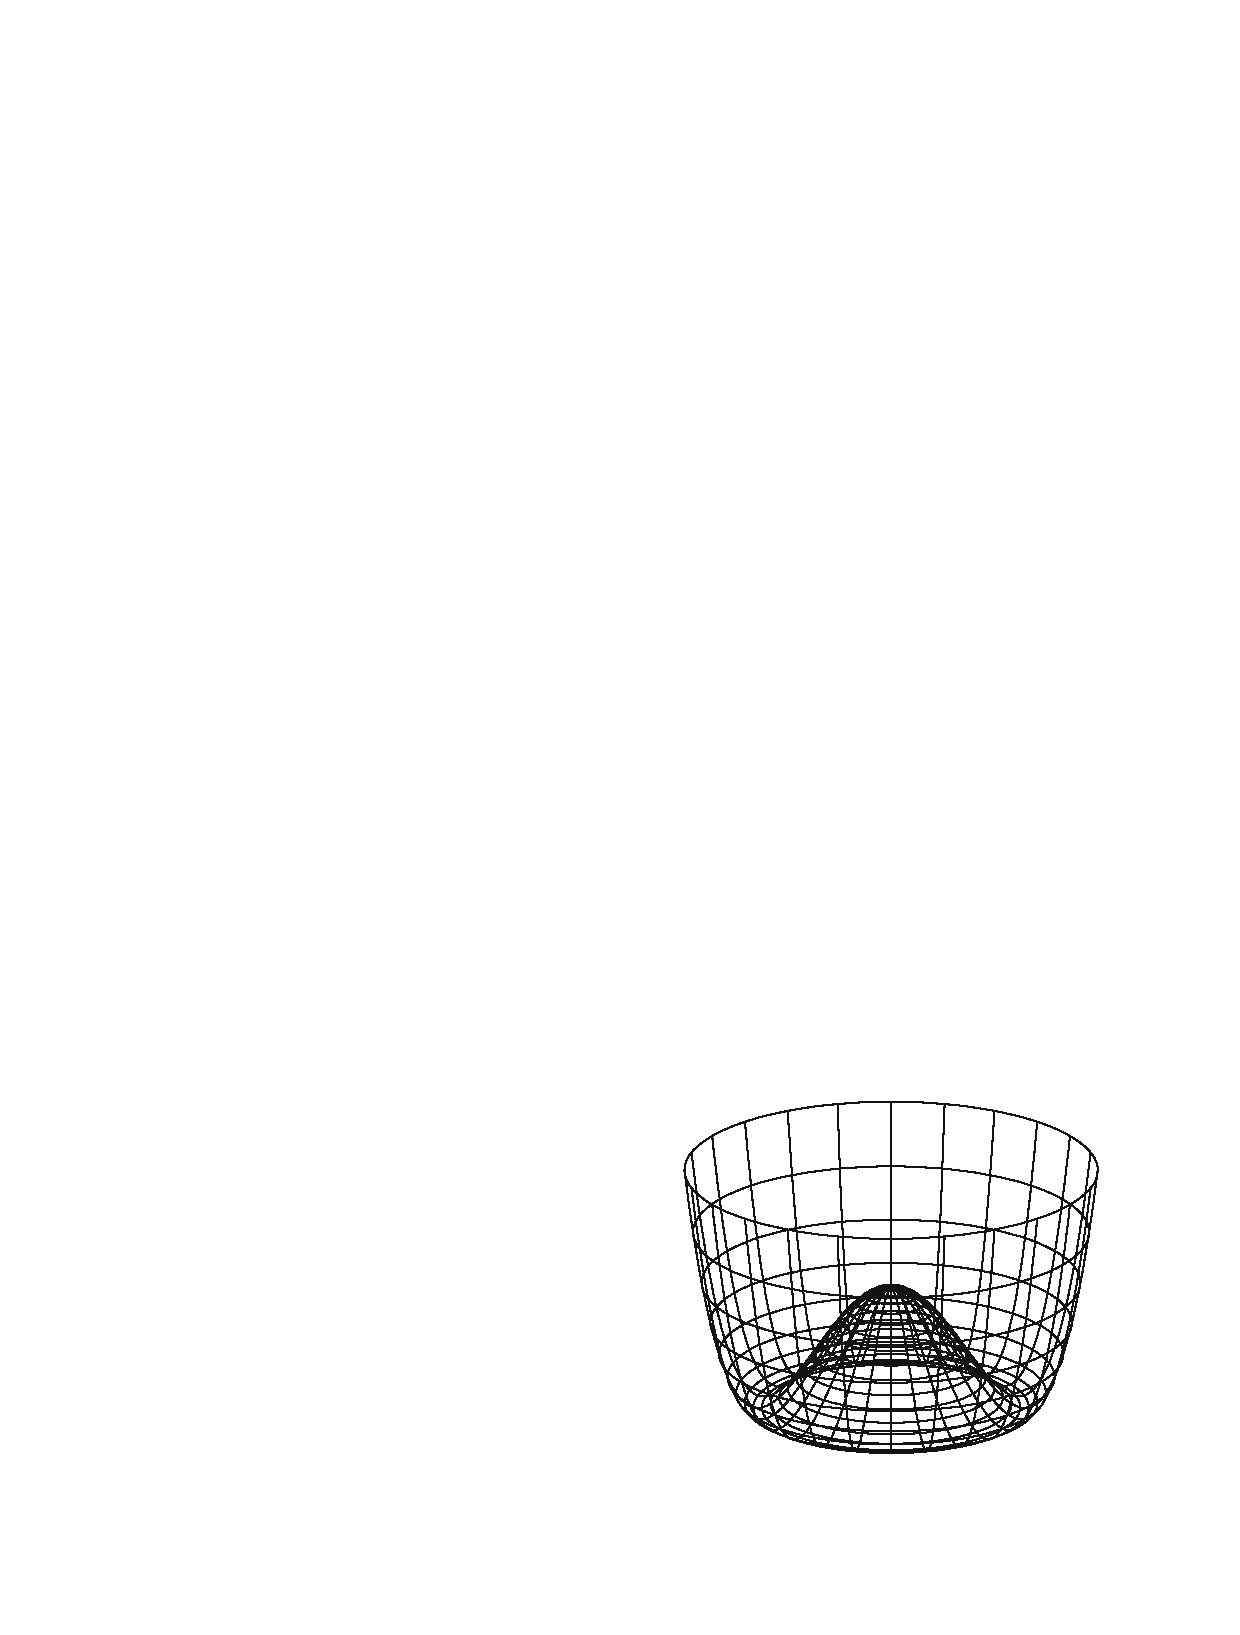
\includegraphics[width=0.5\textwidth]{Higgs_potential}
\caption[The Higgs field potential]{The Higgs field potential in the complex plane, commonly referred to as a
``Mexican hat'' potential \autocite{top_quark_at_HC}}
\label{fig:higgs_potential}
\end{figure}

The choice of minimum corresponding to the lowest energy state (or vacuum) is completely arbitrary. In fact, any point
at which the potential is minimum loses the invariance under $SU(2)_L \times U(1)_Y$ gauge transformations. Therefore,
nature spontaneously breaks the symmetry by picking the vacuum from the set of minima of the Higgs potential.
Conventionally, we can choose
\begin{equation}
\langle 0 | \phi | 0 \rangle = \frac{1}{\sqrt{2}} \twovector{0}{v}.
\label{eq:unitary_gauge_vev}
\end{equation}

Expanding around the chosen minimum, $\phi$ is then given by
\begin{equation}
\phi = \frac{1}{\sqrt{2}} \twovector{0}{v+H},
\end{equation}
where $H$ is the neutral scalar Higgs field. By substituting this field into the Lagrangian in
Equation~\ref{eq:Higgs_L}, one can obtain:
\begin{equation}
\begin{split}
\calL_\textrm{Higgs} & = \frac{1}{2} (\partial_\mu H)(\partial^\mu H) + \frac{1}{4} g^2 (H^2 + 2vH + v^2) W^+_\mu
W^{-\mu} + \\ & + \frac{1}{8} (g^2 + {g'}^2)(H^2 + 2vH + v^2)Z_\mu Z^\mu - \\ & - \mu^2 H^2 - \frac{\lambda}{4} (H^4 +
4vH^3),
\end{split}
\label{eq:Higgs_L_final}
\end{equation}
where physical fields $W^{\pm}_\mu$ and $Z_\mu$ are given by Equations~\ref{eq:W_mu} and \ref{eq:Z_mu}, respectively.
Notably, we can see that these fields have acquired mass terms in the Lagrangian, with the masses of vector bosons given
by
\begin{subequations}
\begin{align}
M_W &= \frac{1}{2}gv, \\
M_Z &= \frac{1}{2}v\sqrt{g^2+{g'}^2} = \frac{1}{2} \frac{gv}{\cos{\theta_W}},
\end{align}
\end{subequations}
whereas the mass of the Higgs boson itself is given by
\begin{equation}
M_H = \sqrt{2} \mu = v \sqrt{2\lambda}.
\end{equation}

% Unlike the \W and \Z boson masses which can be predicted from the measurement of the fine structure constant, the Higgs
% mass $M_H$ can not be determined by other experimentally measured parameters.

% However, it is possible to put indirect constraints on $M_H$ through quantum loop corrections and precise measurement of
% the \W boson and top quark masses. This will be discussed in Section~\ref{s:top_quak_physics}.

Naturally, the photon field $A_\mu$ acquires no mass terms in the Lagrangian. The Higgs mechanism can also be used in a
similar way to generate fermion masses by introducing an $SU(2)_L \times U(1)_Y$ gauge invariant term responsible for
interaction between the Higgs and fermion fields. This additional term in the Standard Model Lagrangian is called
\textit{Yukawa term}, which for the first generation of fermions is given by
\begin{equation}
\calL_\textrm{Yukawa} = -Y_e^{ij} \bar{l_L}^i \phi e_R^j - Y_u^{ij} \bar{q_L}^i \epsilon \phi^\dag u_R^j - Y_d^{ij}
\bar{q_L}^i \phi d_R^j + \textrm{h.c.},
\end{equation}
where coefficients $Y_{e,u,d}^{ij}$ are $3\times3$ complex matrices (Yukawa couplings) and $\epsilon$ is the $2\times2$
antisymmetric tensor. When the Higgs field $\phi$ acquires the vacuum expectation value given by
Equation~\ref{eq:unitary_gauge_vev}, the Yukawa Lagrangian yields mass terms for fermions, generating the masses:
\begin{equation}
M_f = Y_f \frac{v}{\sqrt{2}}.
\end{equation}

The Yukawa couplings are not diagonal in general, which results in mixing between different generations described for
the quarks by the CKM matrix (Equation~\ref{eq:CKM}). Another curious observation is that the fermion masses are
proportional to Yukawa couplings, which essentially represent the interaction strength with the Higgs field. Due to the
large mass of the top quark of approximately \SI{173}{\GeV}, and the Higgs field vacuum expectation value
$v\approx\SI{246}{\GeV}$, the Yukawa coupling to the top quark is very close to unity.

The existence of the Higgs boson and therefore the nature of electroweak symmetry breaking had long remained a mystery.
In the summer of 2012 both ATLAS and CMS experiments at the LHC observed the Higgs boson with an approximate mass of
\SI{125}{\GeV} \autocite{ATLAS_higgs_observation, CMS_higgs_observation}, with couplings consistent with theoretical
predictions \autocite{CMS_Higgs_long_paper, ATLAS_Higgs_couplings}, which proved to be yet another triumph of the
Standard Model.

\section{Shortcomings of the SM and physics beyond the SM}
\label{s:SM_shortcomings}
Despite being the most successful theory up to date, the Standard Model is not perfect and has its shortcomings. There
is a range of physical phenomena not explained by the SM. Let us mention the most prominent ones.

\begin{description}[wide=\parindent]
\item [Gravity] is not included in the Standard Model, as a consistent theory of quantum gravity is yet to be derived.
General relativity, the only accepted theory of gravity, is in fact fundamentally incompatible with quantum mechanics
and therefore the Standard Model.
\item [Massive neutrinos] are also not explained by the SM. The evidence for neutrino oscillations was confirmed by the
Super-Kamiokande collaboration \autocite{neutrino_oscillations}, which necessarily implies that neutrinos are massive
particles. It is possible to include massive neutrinos in some extensions of the Standard Model, whilst also keeping the
local symmetry of weak interactions \autocite{Shaposhnikov_nuMSM}. However, this leads to new theoretical problems
(e.g.\ unnaturally small neutrino Yukawa couplings).
\item [Matter/antimatter asymmetry,] which is apparent in the Universe, is not fully accounted for by the observed CP
violation in the Standard Model \autocite{Peskin_matter_antimatter, matter_antimatter_asymmetry}. Therefore, another
mechanism inducing the matter/antimatter asymmetry must exist, most likely requiring new physics models beyond the
Standard Model.

%\item [Strong CP problem] refers to the absence of any fundamental theoretical prohibition of CP violation in strong
%interactions. However, such strong CP violation has not been observed.
\item [Dark matter and dark energy] constitute approximately \SI{95}{\pc} of the mass/energy content in our Universe,
according to the latest Planck data \autocite{planck2013-p01, planck2013-p11}. The Standard Model only describes the
remaining \SI{5}{\pc} (i.e.\ ordinary matter), whereas the origin of dark matter and dark energy remains unknown.
\end{description}

Furthermore, there is a number of fundamental theoretical issues within the Standard Model, implying the intrinsic
incompleteness of the theory. The SM does not explain why it has only three generations of fermions. Moreover, there is
no explanation for the vast difference between masses of fermions (known as the Flavour problem), hence the origin of
Yukawa couplings (and therefore the CKM matrix) remains an open problem in particle physics.

Additionally, the \textit{ad hoc} nature of the Higgs mechanism gives rise to the hierarchy problem, which is related to
quadratic divergence of the loop corrections to the Higgs boson mass. The Higgs mass is renormalised by loop diagrams
(e.g.\ shown in Figure~\ref{fig:Higgs_loops}), making it extremely large  -- of the order of Planck scale (\SI{\sim
e19}{\GeV}) -- unless there is some unnatural fine tuning involved.

\begin{figure}[!hbtp]
	\centering
	\begin{minipage}[b]{0.4\textwidth}
	\centering
	\subfloat[]{
		\begin{fmfgraph*}(100,50)
		\fmfleft{i}
		\fmfright{o}
		\fmflabel{$H$}{i}
		\fmflabel{$H$}{o}
		\fmf{dashes,tension=3}{i,v1}
		\fmf{dashes,tension=3}{v2,o}
		\fmf{fermion,left,tension=1}{v1,v2,v1}
		\fmfdot{v1,v2}
		\end{fmfgraph*}
	}
	\end{minipage}
	\hspace{1cm}
	\begin{minipage}[b]{0.4\textwidth}
	\centering
	\subfloat[]{
		\begin{fmfgraph*}(100,50)
		\fmfleft{i}
		\fmfright{o}
		\fmflabel{$H$}{i}
		\fmflabel{$H$}{o}
		\fmf{dashes}{i,v1}
		\fmf{dashes}{v1,o}
		\fmffreeze
		\fmf{dashes,tension=1}{v1,v1}
		\fmfdot{v1}
		\end{fmfgraph*}
	}
	\end{minipage}
	\caption[Loop contributions to the Higgs boson mass]{Loop contributions to the Higgs boson mass: (a) fermion loops, (b)
	boson loops.}
  \label{fig:Higgs_loops}
\end{figure}


All these problems motivate the need for new models, referred to as physics beyond the Standard Model (BSM). Most
notable BSM models are briefly mentioned below.

\begin{description}[wide=\parindent]
\item [Supersymmetry] (SUSY) \autocite{SUSY_primer} is an extension of the SM, introducing a supersymmetric partner to
each ordinary particle by varying its spin by $1/2$. Thus, each fermion has a bosonic partner, and all bosons have
fermionic partners. Despite the greater number of free parameters, SUSY offers attractive solutions to most of the
mentioned problems of the SM. For example, the hierarchy problem is naturally solved in SUSY since the loop corrections
are automatically cancelled by corresponding contributions from supersymmetric partners. Most SUSY models also provide
good candidates for Dark Matter.
\item [Extra dimensions] refer to theories containing additional space-time dimensions, in which gravity is allowed to
propagate. This leads to reduction of the hierarchy between the Planck and electroweak scales, thus resolving the
hierarchy problem \autocite{Arkani-Hamed, RS}.
\item [Composite models,] such as topcolour \autocite{topcolour} or composite Higgs \autocite{composite_Higgs} models,
attempt to resolve some of the issues of the Standard Model by either introducing new composite particles or suggesting
a composite nature for the existing particles in the SM.
%\item [Grand Unified Theories (GUTs)] are a range of models striving to unify all fundamental forces.
\end{description}

An important and desirable feature of any physics model is its falsifiability in the accessible energy range. A wide
range of BSM models provide particle candidates that may exhibit themselves at the energy scale accessible at the LHC,
therefore a rich physics programme at the LHC must ensure an active search for all possible signs of new physics.

\newpage
\section{Top Quark Physics within the Standard Model}
\label{s:top_quak_physics}
The top quark is the heaviest elementary particle in the Standard Model, and the heaviest observed particle, discovered
in 1995 at the Tevatron collider by CDF and D{\O} collaborations \autocite{CDF_top_observation, D0_top_observation}. The
large mass of approximately \SI{173}{\GeV} suggests that the top quark may have a special role in nature. It is
substantially more massive than any other fermion. As mentioned in Section~\ref{s:SM_shortcomings}, the reason for such
vast discrepancy between fermion masses is not known. It is also not yet understood why the top quark's Yukawa coupling
to the Higgs boson is so close to unity. Naturally, studying the most massive fermion is a logical starting point in
search for answers to these questions.

Due to its large mass, the top quark has an extremely short lifetime of \SI{\approx5e-25}{\s} \autocite{PDG}, meaning
that it decays before the top-flavoured hadrons or \ttbar bound states can form. Therefore, the spin information is
passed from the top quark on to its decay products, providing a unique possibility to study a ``bare'' quark.
High-precision measurements of the top quark properties, such as mass (Chapter~\ref{c:top_mass_analysis}) and cross
section (Chapter~\ref{c:xsection_analysis}) are important tools to test the Standard Model and probe for new physics
beyond it.

\subsection{Top quark production at the LHC}
\label{ss:top_production}
There are two particular mechanisms of top quark production in hadron collisions: top-antitop (\ttbar) pair production
via the strong interaction, and single top quark production via the electroweak interaction. The \ttbar production
dominates over single top production, being the main source of top quarks at the LHC, and therefore is the main focus of
this thesis.

Feynman diagrams for \ttbar production to leading order are presented in
Figure~\ref{fig:ttbar_production_feynman_diagrams}. At the LHC, the major process for \ttbar production is gluon fusion,
constituting approximately \SI{90}{\pc} (\SI{80}{\pc}) at $\sqrt s =$ \SI{14}{\TeV} (\SI{7}{\TeV}) \autocite{PDG}.
Quark-antiquark annihilation and higher-order processes contribute the rest of the Standard Model \ttbar production.
This happens due to the fact that the LHC is a proton-proton collider, and the only source of antiquarks are virtual
quarks (so-called sea quarks). At the Tevatron, which was a proton-antiproton collider, the quark-antiquark annihilation
was the main \ttbar production mode.

\begin{figure}[!htbp]
	\begin{minipage}[t]{0.49\textwidth}
	\centering
	\subfloat[]{
		\begin{fmfgraph*}(150,75)
		\fmfleft{i1,i2}
		\fmfright{o1,o2}
		\fmflabel{$g$}{i1}
		\fmflabel{$g$}{i2}
		\fmflabel{$\bar{t}$}{o1}
		\fmflabel{$t$}{o2}

		\fmf{gluon}{i1,v1}
		\fmf{gluon}{i2,v2}
		\fmf{fermion}{v1,v2}
		\fmf{fermion}{o1,v1}
		\fmf{fermion}{v2,o2}
		\end{fmfgraph*}
	}
	\end{minipage}
	\hfill
	\begin{minipage}[t]{0.49\textwidth}
	\centering
	\subfloat[]{
		\begin{fmfgraph*}(150,75)
		\fmfleft{i1,i2}
		\fmfright{o1,o2}
		\fmflabel{$g$}{i1}
		\fmflabel{$g$}{i2}
		\fmflabel{$\bar{t}$}{o1}
		\fmflabel{$t$}{o2}

		\fmf{gluon}{i1,v1}
		\fmf{gluon}{i2,v1}
		\fmf{gluon}{v1,v2}
		\fmf{fermion}{o1,v2}
		\fmf{fermion}{v2,o2}
		\end{fmfgraph*}
	}
	\end{minipage}

	\vspace{1cm}

	\begin{minipage}[t]{0.49\textwidth}
	\centering
	\subfloat[]{
		\begin{fmfgraph*}(150,75)
		\fmfleft{i1,i2}
		\fmfright{o1,o2}
		\fmflabel{$g$}{i1}
		\fmflabel{$g$}{i2}
		\fmflabel{$\bar{t}$}{o1}
		\fmflabel{$t$}{o2}

		\fmf{gluon}{i1,v1}
		\fmf{phantom}{v1,o1}
		\fmf{gluon}{i2,v2}
		\fmf{phantom}{v2,o2}
		\fmf{fermion}{v2,v1}

		\fmf{fermion,tension=0}{v1,o2}
		\fmf{fermion,tension=0}{o1,v2}

		\end{fmfgraph*}
	}
	\end{minipage}
	\hfill
	\begin{minipage}[t]{0.49\textwidth}
	\centering
	\subfloat[]{
		\begin{fmfgraph*}(150,75)
		\fmfleft{i1,i2}
		\fmfright{o1,o2}
		\fmflabel{$\bar{q}$}{i1}
		\fmflabel{$q$}{i2}
		\fmflabel{$\bar{t}$}{o1}
		\fmflabel{$t$}{o2}

		\fmf{fermion}{v1,i1}
		\fmf{fermion}{i2,v1}
		\fmf{gluon}{v1,v2}
		\fmf{fermion}{o1,v2}
		\fmf{fermion}{v2,o2}
		\end{fmfgraph*}
	}
	\end{minipage}

	\caption[Feynman diagrams for leading order \ttbar production at the LHC]{Feynman diagrams for leading order \ttbar
	production at the LHC: (a), (b) and (c) show the gluon fusion, the dominant production mechanism, (d) represents
	quark-antiquark annihilation.}
  \label{fig:ttbar_production_feynman_diagrams}
\end{figure}

Figure~\ref{fig:single_top_production_feynman_diagrams} shows the Feynman diagrams of various single top production
modes. Three major production mechanisms include s-channel and t-channel \W boson exchange, and associated production
with a \W boson (tW-channel). Measurement of single top production is of significant interest since it allows the direct
measurement of the Wtb vertex and therefore the magnitude of $|V_{tb}|$ element of the CKM matrix.

\begin{figure}[!hbtp]
	\centering
	\vspace*{0.5cm}
	\begin{minipage}[b]{0.3\textwidth}
	\centering
	\subfloat[]{
		\begin{fmfgraph*}(150,75)
		\fmfleft{i1,i2}
		\fmfright{o1,o2}
		\fmflabel{$q$}{i1}
		\fmflabel{$\bar{q}'$}{i2}
		\fmflabel{$\bar{b}$}{o1}
		\fmflabel{$t$}{o2}

		\fmf{fermion}{i1,v1}
		\fmf{fermion}{v1,i2}
		\fmf{photon, label=$W$}{v1,v2}
		\fmf{fermion}{o1,v2}
		\fmf{fermion}{v2,o2}
		\end{fmfgraph*}
	}
	\end{minipage}
	\hfill
	\begin{minipage}[b]{0.3\textwidth}
	\centering
	\subfloat[]{
		\begin{fmfgraph*}(150,75)
		\fmfleft{i1,i2}
		\fmfright{o1,o2,o3}
		\fmflabel{$g$}{i1}
		\fmflabel{$q$}{i2}
		\fmflabel{$\bar{b}$}{o1}
		\fmflabel{$t$}{o2}
		\fmflabel{$q'$}{o3}

		\fmf{gluon}{i1,v1}
		\fmf{fermion}{i2,v3}
		\fmf{fermion, label=$b$}{v1,v2}
		\fmf{photon, label=$W$}{v2,v3}
		\fmf{fermion}{o1,v1}
		\fmf{fermion}{v2,o2}
		\fmf{fermion}{v3,o3}
		\end{fmfgraph*}
	}
	\end{minipage}
	\hfill
	\begin{minipage}[b]{0.3\textwidth}
	\centering
	\subfloat[]{
		\begin{fmfgraph*}(150,75)
		\fmfleft{i1,i2}
		\fmfright{o1,o2}
		\fmflabel{$b$}{i1}
		\fmflabel{$q$}{i2}
		\fmflabel{$t$}{o1}
		\fmflabel{$q'$}{o2}

		\fmf{fermion}{i1,v1}
		\fmf{fermion}{i2,v2}
		\fmf{photon, label=$W$}{v1,v2}
		\fmf{fermion}{v1,o1}
		\fmf{fermion}{v2,o2}
		\end{fmfgraph*}
	}
	\end{minipage}

	\vspace{1cm}

	\hfill

	\begin{minipage}[t]{0.3\textwidth}
	\centering
	\subfloat[]{
		\begin{fmfgraph*}(150,75)
		\fmfleft{i1,i2}
		\fmfright{o1,o2}
		\fmflabel{$g$}{i1}
		\fmflabel{$b$}{i2}
		\fmflabel{$t$}{o1}
		\fmflabel{$W$}{o2}

		\fmf{gluon}{i1,v1}
		\fmf{fermion}{i2,v1}
		\fmf{fermion, label=$b$}{v1,v2}
		\fmf{fermion}{v2,o1}
		\fmf{photon}{v2,o2}
		\end{fmfgraph*}
	}
	\end{minipage}
	\hspace{2cm}
	\begin{minipage}[t]{0.3\textwidth}
	\centering
	\subfloat[]{
		\begin{fmfgraph*}(150,75)
		\fmfleft{i1,i2}
		\fmfright{o1,o2}
		\fmflabel{$b$}{i1}
		\fmflabel{$g$}{i2}
		\fmflabel{$W$}{o1}
		\fmflabel{$t$}{o2}

		\fmf{fermion}{i1,v1}
		\fmf{gluon}{i2,v2}
		\fmf{fermion, label=$t$}{v1,v2}
		\fmf{photon}{v1,o1}
		\fmf{fermion}{v2,o2}
		\end{fmfgraph*}
	}
	\end{minipage}
	\hfill

	\caption[Feynman diagrams for leading order single top production]{Feynman diagrams for leading order
	single top production. (a) s-channel, (b) and (c) t-channel, (d) and (e) tW-channel.}
  \label{fig:single_top_production_feynman_diagrams}
\end{figure}

\subsection{Top quark decay}
\label{ss:top_decay}
The top quark predominantly decays to a \W boson and a b-quark: $\cPqt \rightarrow \W \cPqb$. Other possible decay modes
($\cPqt \rightarrow \W \cPqs$ and $\cPqt \rightarrow \W \cPqd$) are suppressed in the Standard Model by the unitarity
requirement of the CKM matrix, which yields \autocite{PDG} the $|V_{tb}|$ value of
\begin{equation}
|V_{tb}| = 0.999146^{+0.000021}_{-0.000046}.
\end{equation}

As it was previously mentioned, the direct measurement of $|V_{tb}|$ (without assuming unitarity) can be performed by
measuring the single top production cross section. The recent CMS result is consistent with the Standard
Model \autocite{single_top_Vtb_CMS}:
\begin{equation}
|V_{tb}| = 0.998 \pm 0.038~\textrm{(experimental)} \pm 0.016~\textrm{(theoretical)}.
\end{equation}

The branching fraction of $\cPqt \rightarrow \W \cPqb$ decay is assumed to be \SI{100}{\pc} hereafter. Therefore, the
\ttbar decay modes completely depend on subsequent \W boson decays:
\begin{itemize}
  \item fully hadronic: \ttbar $\rightarrow \cPqb \W^+ ~ \bar{\cPqb} \W^- \rightarrow  \cPqb~\cPq\bar{\cPq}' ~
  \bar{\cPqb}~\cPq'' \bar{\cPq}'''$ (\SI{45.7}{\pc});
  \item semileptonic: \ttbar $\rightarrow \cPqb \W^+ ~ \bar{\cPqb} \W^- \rightarrow \cPqb~\cPq\bar{\cPq}' ~ \bar{\cPqb}
  ~ l^- \bar{\nu}_l + \cPqb~l^+ \nu_l ~ \bar{\cPqb}~\cPq'' \bar{\cPq}'''$ (\SI{43.8}{\pc});
  \item dileptonic: \ttbar $\rightarrow \cPqb \W^+ ~ \bar{\cPqb} \W^- \rightarrow  \cPqb~\bar{l} \nu_l ~ \bar{\cPqb} ~
  l'\bar{\nu}_{l'}$ (\SI{10.5}{\pc}).
\end{itemize}

Percentages in parentheses show the branching fractions corresponding to the decay modes \autocite{PDG}. The quarks in
all final states hadronise into jets. The number of jets is not limited to the number of initial quarks due to the
contribution from extra QCD radiation (i.e.\ gluon radiation) either before or after \ttbar production.

The fully hadronic \ttbar decay signature implies at least 6 jets in the final state and no leptons, hence it is heavily
contaminated by the background from QCD and \W/\ZpJets processes. Dileptonic \ttbar decay has a clean signature, but due
to the lowest branching fraction can suffer from limited statistics. The semileptonic decay mode, shown in
Figure~\ref{fig:ttbar_semileptonic_decay}, has exactly one highly energetic lepton and at least four jets in the final
state, which is therefore called the lepton plus jets final state. The lepton can be an electron, a muon or a
$\tau$-lepton; however, since the $\tau$-leptons are difficult to reconstruct, they are usually excluded from top quark
analyses studying semileptonic decays. Analyses in this thesis study the electron plus jets ($e+$jets) and muon plus
jets ($\mu+$jets) decay channels, which have branching fractions of \SI{\approx14}{\pc} each.

\begin{figure}[!hbtp]
	\centering
	\vspace*{0.5cm}
	\begin{fmfgraph*}(300,150)
	\fmfleft{i1,i2,i3}
	\fmfright{o1,o2,o3}
	\fmflabel{$\bar{q}$}{i1}
	\fmflabel{$q$}{i2}
	\fmflabel{$\bar{b}$}{i3}
	\fmflabel{$b$}{o1}
	\fmflabel{$l^+$}{o2}
	\fmflabel{$\nu_l$}{o3}
	
	\fmf{fermion}{i3,v2}
	\fmf{phantom}{i1,v2}
	\fmf{fermion, label=$\bar{t}$}{v2,v3}
	\fmf{fermion, label=$t$}{v3,v4}
	\fmf{fermion}{v4,o1}
	\fmf{phantom}{o3,v4}
	\fmffreeze
	\fmf{fermion}{i1,v1}
	\fmf{fermion}{v1,i2}
	\fmf{fermion}{o2,v5}
	\fmf{fermion}{v5,o3}
	\fmf{photon, label=$W^-$}{v1,v2}
	\fmf{photon, label=$W^+$}{v4,v5}
	\fmfdot{v3}
	\end{fmfgraph*}
	\caption{Semileptonic \ttbar decay mode}
  \label{fig:ttbar_semileptonic_decay}
\end{figure}


\newpage
\subsection{Background processes to semileptonic top quark pair decay}
\label{ss:backgrounds}
Both top quark mass and differential cross section analyses presented in this thesis are based on selection of events
with semileptonic ($e/\mu+$jets) \ttbar decay signature. Being relatively clean yet still providing sufficient event
yields, this decay mode is used in many measurements of top quark properties, and is often called a ``golden channel''
in top quark physics. Good understanding of background contributions is very important for accuracy and reliability of
measurements. The most significant background processes to semileptonic \ttbar decay are described below.

\subsubsection*{Single top quark background}
One of the less significant backgrounds to lepton plus jets analyses is the single top quark production. Major
production modes for this process (mentioned in Section~\ref{ss:top_production}) have a lower number of jets in the
final state than that of the \ttbar production, however, additional jets can emerge from inital and final state
radiation (ISR/FSR), i.e.\ soft gluon radiation before and after the hard scattering process. This contribution is not
negligible, and is modelled using Monte Carlo simulation.

\subsubsection*{\WpJets background}
Production of \W bosons with additional jets (called \WpJets) is one of the most significant backgrounds to semileptonic
\ttbar decays. Example Feynman diagrams for leading order \W boson production are shown in
Figure~\ref{fig:VJets_processes} (a, b). Leptonic decays in the \WpJets process together with extra jets can
successfully mimic the \ttbar decay since it also includes two \W bosons. However, leptons and jets in \WpJets processes
are usually much softer than those coming from \ttbar decay, due to the large mass of top quarks. Moreover, additional
jets are less likely to be \cPqb-jets which are necessarily present in \ttbar decay. Therefore, tagging of \cPqb-jets
and high kinematic cuts on lepton and jets transverse momenta can significantly reduce the
\WpJets background. Besides, the production cross section of \WpJets events reduces exponentially with increasing number
of jets \autocite{multijet_WZ}, therefore jet multiplicity cuts also help to mitigate this background. These methods are
detailed in selection procedures of top quark mass and differential cross section analyses in
Sections~\ref{s_top_mass:event_selection} and \ref{s_xsection:event_selection}, respectively.

\subsubsection*{\ZpJets background}
\Z boson production processes with additional jets (\ZpJets) are largely similar to \WpJets processes, as can be seen in
Figure~\ref{fig:VJets_processes} (c, d). The difference lies in leptonic decays of the \Z boson, as it produces two
opposite-sign leptons. Vetoing the second lepton in the selection is therefore particularly helpful in reducing this
background. Contamination can still occur if one of the leptons is misreconstructed as a jet or does not pass
identification criteria. This contribution is estimated to be small, and together with the jet multiplicity cuts the
\ZpJets background is usually mitigated significantly.

\begin{figure}[tbp]
	\begin{minipage}[t]{0.49\textwidth}
	\centering
	\subfloat[]{
		\begin{fmfgraph*}(150,75)
		\fmfleft{i1,i2}
		\fmfright{o1,o2}
		\fmflabel{$q$}{i1}
		\fmflabel{$g$}{i2}
		\fmflabel{$q'$}{o1}
		\fmflabel{$W$}{o2}

		\fmf{fermion}{i1,v1}
		\fmf{gluon}{i2,v1}
		\fmf{fermion}{v1,v2}
		\fmf{fermion}{v2,o1}
		\fmf{photon}{v2,o2}
		\end{fmfgraph*}
	}
	\end{minipage}
	\hfill
	\begin{minipage}[t]{0.49\textwidth}
	\centering
	\subfloat[]{
		\begin{fmfgraph*}(150,75)
		\fmfleft{i1,i2}
		\fmfright{o1,o2}
		\fmflabel{$q$}{i1}
		\fmflabel{$\bar{q}'$}{i2}
		\fmflabel{$g$}{o1}
		\fmflabel{$W$}{o2}

		\fmf{fermion}{i1,v1}
		\fmf{fermion}{v2,i2}
		\fmf{fermion}{v1,v2}
		\fmf{gluon}{v1,o1}
		\fmf{photon}{v2,o2}
		\end{fmfgraph*}
	}
	\end{minipage}

	\vspace{1cm}

	\begin{minipage}[t]{0.49\textwidth}
	\centering
		\subfloat[]{
		\begin{fmfgraph*}(150,75)
		\fmfleft{i1,i2}
		\fmfright{o1,o2}
		\fmflabel{$q$}{i1}
		\fmflabel{$g$}{i2}
		\fmflabel{$q'$}{o1}
		\fmflabel{$Z$}{o2}

		\fmf{fermion}{i1,v1}
		\fmf{gluon}{i2,v1}
		\fmf{fermion}{v1,v2}
		\fmf{fermion}{v2,o1}
		\fmf{photon}{v2,o2}
		\end{fmfgraph*}
	}
	\end{minipage}
	\hfill
	\begin{minipage}[t]{0.49\textwidth}
	\centering
	\subfloat[]{
		\begin{fmfgraph*}(150,75)
		\fmfleft{i1,i2}
		\fmfright{o1,o2}
		\fmflabel{$g$}{i1}
		\fmflabel{$q$}{i2}
		\fmflabel{$q'$}{o1}
		\fmflabel{$Z$}{o2}

		\fmf{gluon}{i1,v1}
		\fmf{fermion}{i2,v2}
		\fmf{fermion}{v2,v1}
		\fmf{fermion}{v1,o1}
		\fmf{photon}{v2,o2}
		\end{fmfgraph*}
	}
	\end{minipage}

	\caption[Example diagrams for leading order \W and \Z boson production at the
	LHC.]{Example diagrams for leading order \W boson (a, b) and \Z boson (c,
	d) production at the LHC.}
  \label{fig:VJets_processes}
\end{figure}

\subsubsection*{QCD multi-jet background}
Standard QCD processes in hadron collisions, such as gluon fusion and quark-antiquark annihilation, usually result in
production of highly energetic jets. Examples of these processes in the lowest order with two jets in the final state
are shown in Figure~\ref{fig:QCD_processes}. Additional jets arise at higher orders and can potentially fake \ttbar
signal. Although QCD events do not produce real prompt leptons, this can happen when jets are mis-identified as leptons.
These objects are referred to as fake leptons. Due to strict identification criteria of real electrons and muons
(described in Sections~\ref{ss:electron_reconstruction} and \ref{ss:muon_reconstruction}), such mis-identifications are
extremely rare. However, since the production cross section of QCD events is very large, this background becomes
considerable.

\begin{figure}[tbp]
	\begin{minipage}[t]{0.49\textwidth}
	\centering
	\subfloat[]{
		\begin{fmfgraph*}(150,75)
		\fmfleft{i1,i2}
		\fmfright{o1,o2}
		\fmflabel{$q$}{i1}
		\fmflabel{$g$}{i2}
		\fmflabel{$\bar{q}$}{o1}
		\fmflabel{$q$}{o2}

		\fmf{gluon}{i1,v1}
		\fmf{gluon}{i2,v1}
		\fmf{gluon}{v1,v2}
		\fmf{fermion}{o1,v2}
		\fmf{fermion}{v2,o2}
		\end{fmfgraph*}
	}
	\end{minipage}
	\hfill
	\begin{minipage}[t]{0.49\textwidth}
	\centering
	\subfloat[]{
		\begin{fmfgraph*}(150,75)
		\fmfleft{i1,i2}
		\fmfright{o1,o2}
		\fmflabel{$q$}{i1}
		\fmflabel{$g$}{i2}
		\fmflabel{$g$}{o1}
		\fmflabel{$g$}{o2}

		\fmf{gluon}{i1,v1}
		\fmf{gluon}{i2,v1}
		\fmf{gluon}{v1,v2}
		\fmf{gluon}{o1,v2}
		\fmf{gluon}{v2,o2}
		\end{fmfgraph*}
	}
	\end{minipage}

	\vspace{1cm}

	\begin{minipage}[t]{0.49\textwidth}
	\centering
		\subfloat[]{
		\begin{fmfgraph*}(150,75)
		\fmfleft{i1,i2}
		\fmfright{o1,o2}
		\fmflabel{$q$}{i1}
		\fmflabel{$g$}{i2}
		\fmflabel{$g$}{o1}
		\fmflabel{$q$}{o2}

		\fmf{fermion}{i1,v1}
		\fmf{gluon}{i2,v1}
		\fmf{fermion}{v1,v2}
		\fmf{gluon}{v2,o1}
		\fmf{fermion}{v2,o2}
		\end{fmfgraph*}
	}
	\end{minipage}
	\hfill
	\begin{minipage}[t]{0.49\textwidth}
	\centering
	\subfloat[]{
		\begin{fmfgraph*}(150,75)
		\fmfleft{i1,i2}
		\fmfright{o1,o2}
		\fmflabel{$q'$}{i1}
		\fmflabel{$q$}{i2}
		\fmflabel{$q'$}{o1}
		\fmflabel{$q$}{o2}

		\fmf{fermion}{i1,v1}
		\fmf{fermion}{i2,v2}
		\fmf{gluon}{v2,v1}
		\fmf{fermion}{v1,o1}
		\fmf{fermion}{v2,o2}
		\end{fmfgraph*}
	}
	\end{minipage}

	\caption[Example diagrams for leading order QCD multi-jet production at
	the LHC.]{Example diagrams for leading order QCD multi-jet production at
	the LHC.}
  \label{fig:QCD_processes}
\end{figure}

QCD multi-jet background is usually less significant in the muon plus jets channel, since jets faking muons are easier
to recognise. For instance, when a highly energetic jet punches through the calorimetry system into muon chambers and
thus becomes a fake muon, it can be removed by isolation criteria as it also leaves a significant energy deposit in
calorimeters. Muons (and electrons) can also arise from heavy flavour decays of \cPqb and \cPqc quarks -- these are in
fact real leptons, but as they don't originate at the interaction point, they can be removed by track quality cuts most
of the time.

In the electron plus jets channel, QCD multi-jet background is more prominent. This happens mainly due to photon
conversions, which occur when photons convert into electron-positron pairs. Photons can arise from prompt production
($\gamma+$jets), particle decays or bremsstrahlung radiation. Different methods of identifying such conversions have
been developed, which is discussed in detail in Section~\ref{sss:photon_conversions}.

Due to the large contribution from higher-order processes in signal region, the QCD background is very hard to model.
Large uncertainties in theoretical cross section and potential mismodelling of higher-order effects may lead to biases
in kinematic distributions based on Monte Carlo simulation, as well as in overall acceptance of QCD events passing the
signal selection. Therefore, data-driven methods of QCD background estimation are often preferable (see
Section~\ref{s_xsection:data_driven_QCD}).

\subsubsection*{Additional backgrounds}
Other background processes potentially mimicking semileptonic \ttbar decay include the Drell-Yan process with dilepton
production ($q \bar{q} \rightarrow \Z/\gamma^* \rightarrow l \bar{l}$), and diboson production. The background
contamination from these processes can be reduced by vetoing the second lepton, and is generally considered negligible
due to relatively small production cross sections of these processes.


\subsection{Top quark mass}
\label{ss:top_mass}
The top quark mass is a fundamental parameter of the Standard Model. However, its precise definition is a very
non-trivial problem, ultimately subject to convention. One of the most popular definitions is the pole mass,
corresponding to the real part of a pole in the perturbative propagator of a particle
\autocite{pole_mass_in_QCD_Tarrach}. For the top quark, the perturbative propagator with a four-momentum $p$ has a pole
at \autocite{top_pole_mass}:
\begin{equation}
\sqrt{p^2} = \mtop - \frac{i}{2} \Gamma_\textrm{t},
\end{equation}
where \mtop is the pole mass and $\Gamma_\textrm{t}~\SI{\approx1.5}{\GeV}$ is the top quark decay width. This definition
yields a peak in the invariant mass distribution of the top quark decay products (i.e.\ \W boson and \cPqb-quark), which
is accessible experimentally. As $\mtop \gg \Gamma_\textrm{t}/2$, the peak approximately corresponds to the pole mass,
therefore it is usually assumed that experimentally measured top quark mass represents the pole mass. As will be
discussed later, there are a few problems with this approach.

It has been shown \autocite{pole_mass_in_QCD_Kronfeld} that the pole mass is infrared finite and gauge-invariant to all
orders of perturbative QCD. Despite being well-defined in perturbation theory, an all-order resummation of a particular
class of diagrams known as ``infrared renormalons'' \autocite{renormalons1, renormalons2} leads to an intrinsic
ambiguity of the top quark pole mass proportional to the energy scale of a strong interaction
$\Lambda_\textrm{QCD}~\SI{\approx200}{\MeV}$
\autocite{pole_MS_top_difference}.

Another frequently used mass definition which is free from renormalon ambiguity is the renormalised mass $\MSmtop(\mu)$
in the minimal subtraction (\MS) renormalisation scheme. This mass definition is often call a running mass, since it
depends on the renormalisation scale $\mu$ which is in principle arbitrary. For a choice of $\mu=\MSmtop$, the \MS mass
\MSmtop is related to the pole mass \mtop as follows
\autocite{top_pole_mass}:
\begin{equation}
\mtop = \MSmtop(\MSmtop) \left( 1 + \frac{4}{3} \frac{\overline{\alpha}_S(\MSmtop)}{\pi} + 8.28
\left(\frac{\overline{\alpha}_S(\MSmtop)}{\pi} \right)^2 + ... \right) + \bigO(\Lambda_\textrm{QCD}).
\end{equation}
% \footnote{Renormalisation is a technique of cancelling divergences (infinities) in perturbative quantum field theories.
% Initially infinite parameters become finite after renormalisation, thus acquiring physical sense.}

The difference between the pole mass and the \MS mass is then estimated to be on the order of \SI{10}{\GeV} (with $\mtop
> \MSmtop$). However, it has recently been shown \autocite{pole_MS_top_difference} that including electroweak
corrections for a Higgs boson mass of \SI{\sim125}{\GeV} mostly cancels the corresponding QCD corrections, reducing the
$\mtop-\MSmtop$ difference down to \SI{\sim1}{\GeV}. Theoretical research such as studying higher-order corrections is
actively ongoing in this field.

It has been argued that the top quark mass measured at hadron colliders is in fact a parameter of Monte Carlo
generators, which does not necessarily correspond to the pole mass. This parameter is determined by (next to) leading
order calculations of the matrix elements of hard processes (see Section~\ref{s:MC_simulation}), and this mass
definition does not absorb any corrections from parton showers and hadronisation. Therefore, the actual mass definition
measured experimentally remains not fully understood, with a conceptual uncertainty on the order of
\SI{1}{\GeV} \autocite{measured_top_mass_interpretation}.

Nevertheless, experimental measurements of the top quark mass are of paramount importance. Continuously increasing
precision of the measurements is challenging the current definition of the measured mass, undoubtedly triggering more
effort in reaching a more precise theoretical specification of the mass parameter used in Monte Carlo simulation. As the
top quark is a major background to many new physics searches beyond the Standard Model, deep understanding of its mass
parameter in simulation as well as pushing down the corresponding theoretical and experimental uncertainties are
extremely important.

Nearly 20 years of the Tevatron operation resulted in a very good understanding of the machine and detectors, leading to
an impressively small systematic uncertainty on the top quark mass measurement. The latest combination result from the
Tevatron gives \autocite{tevatron_top_mass_combination}:
\begin{equation}
\mtop = 173.20 \pm 0.51~\textrm{(stat.)} \pm 0.71~\textrm{(syst.)}~\textrm{GeV}.
\end{equation}

The LHC experiments have reached nearly as good precision, with a statistical uncertainty being expectedly smaller
than that of the Tevatron, however, with a larger systematic error due still improving understanding of detector
effects. The latest LHC combination result yields \autocite{LHC_top_mass_combination}:
\begin{equation}
\mtop = 173.29 \pm 0.23~\textrm{(stat.)} \pm 0.92~\textrm{(syst.)}~\textrm{GeV}.
\end{equation}

Recently, the first world combination result of both LHC and Tevatron measurements has become available
\autocite{world_top_mass_combination}:
\begin{equation}
\mtop = 173.34 \pm 0.27~\textrm{(stat.)} \pm 0.71~\textrm{(syst.)}~\textrm{GeV},
\end{equation}
which corresponds to a total uncertainty on the top quark mass of \SI{0.76}{\GeV}, or \SI{0.44}{\pc}. All these results
compared with contributions of individual mass measurements are shown in Figure~\ref{fig:top_mass_world_combination}.

At a proposed linear electron-positron collider (International Linear Collider, ILC), the uncertainty on the top quark
mass is expected to fall below \SI{200}{\MeV}, i.e.\ the energy scale of the strong interaction $\Lambda_\textrm{QCD}$.
It will clearly challenge the theoretical understanding of different mass schemes, ultimately leading to more vigorous
tests of the Standard Model and potentially providing sensitivity to new physics models.

\begin{figure}[hbtp]
   \centering
   {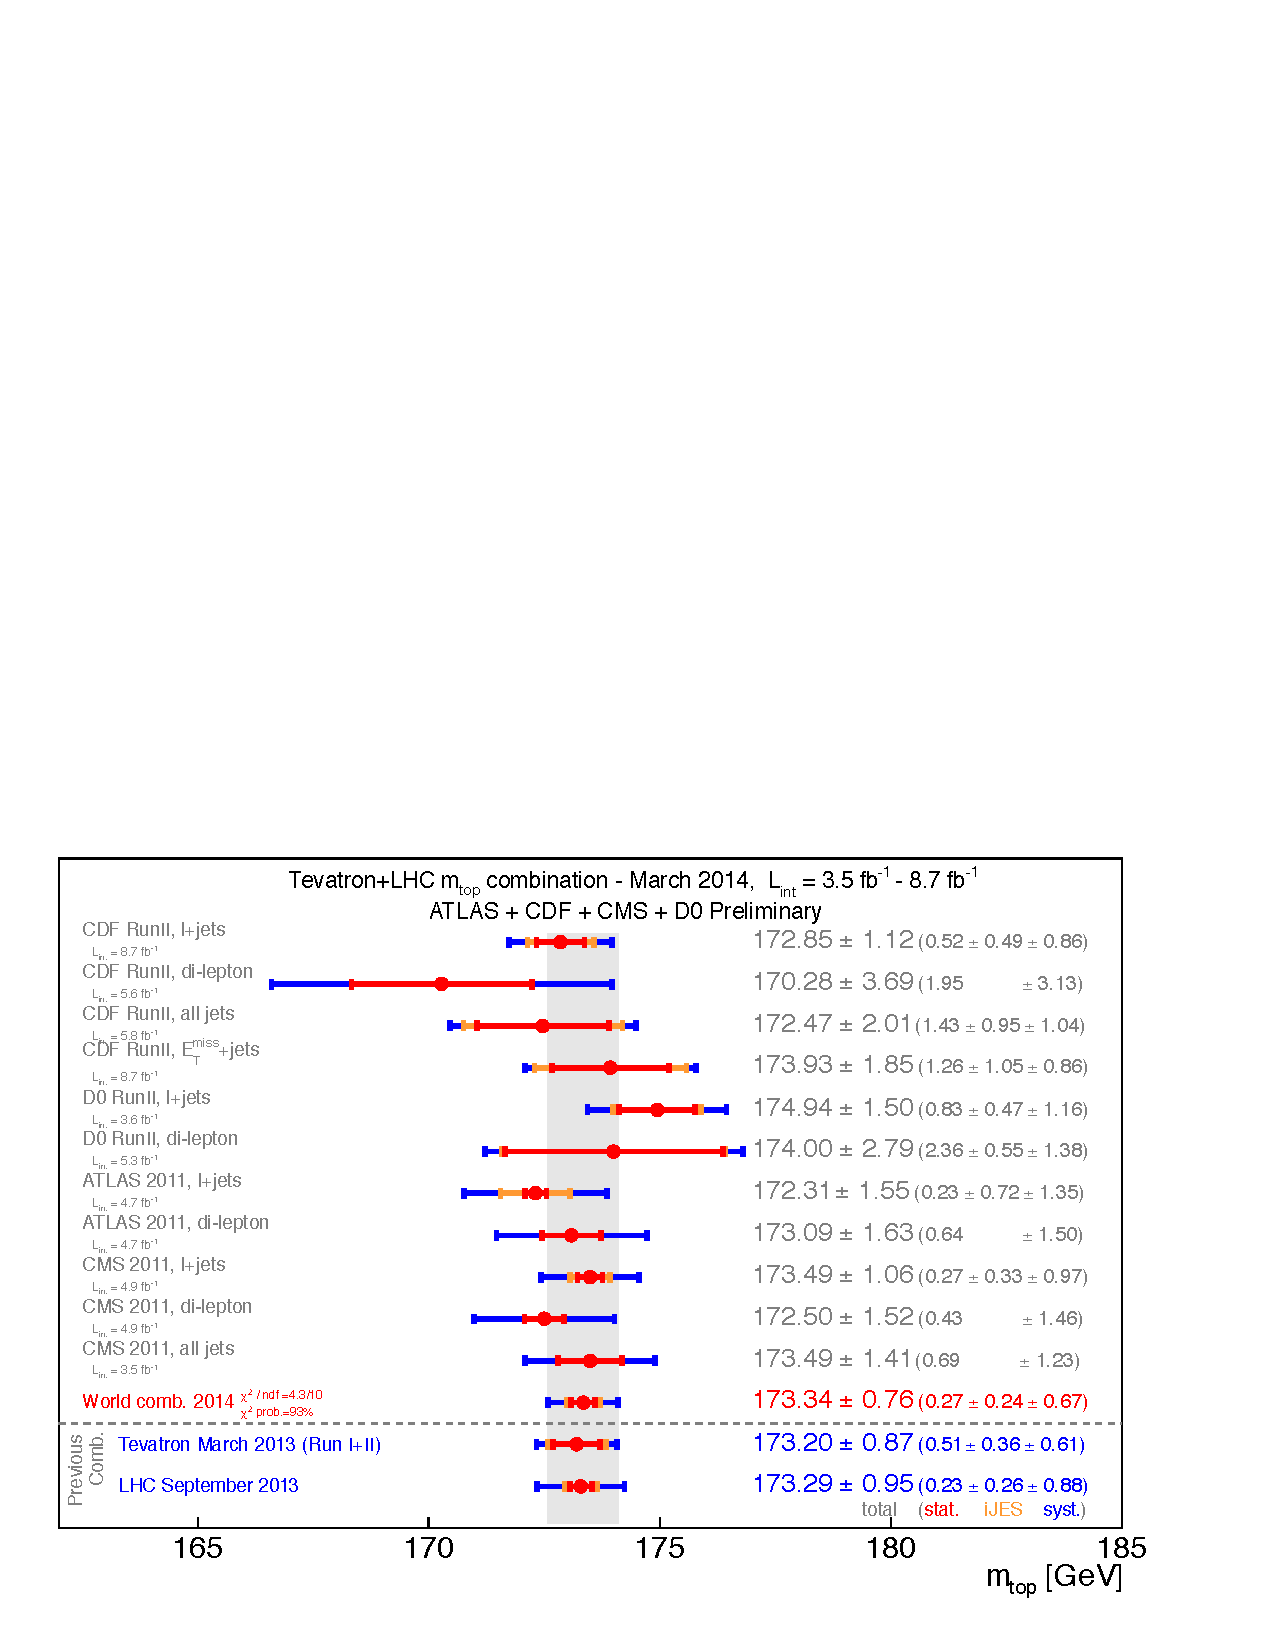
\includegraphics[width=0.9\textwidth]{top_world_combination}}
   \caption[World combination of the top quark mass measurements.]{Top quark mass measurements and the result of their
   combination, compared with the Tevatron and LHC combinations. Each measurement is shown with the total uncertainty,
   the statistical, the jet energy scale (iJES, when applicable), and the systematic uncertainty. The iJES contribution
   is statistical in nature and applies only to analyses performing \textit{in situ} jet energy calibration procedures.
   The grey vertical band shows the total uncertainty on the combined value of the top quark mass
   \autocite{world_top_mass_combination}.}
   \label{fig:top_mass_world_combination}
\end{figure}

\subsection{Top quark pair production cross section}
\label{ss:ttbar_cross_section}
The \ttbar production is a strong interaction process, and therefore is described by perturbative QCD. Hadron collisions
at the LHC (or other hadron colliders) are best viewed as interactions between their constituent quarks and gluons, also
referred to as partons. Since collisions occur at high energies, these interactions result in hard scattering processes
between incoming partons, meaning those involving a significant momentum transfer comparing to the proton mass, and
potentially giving rise to highly energetic final states like top quarks. Each incoming parton carries only a fraction
$x$ of the total momentum of a parent hadron. The distribution of momentum fractions for all flavours of partons are
described by parton distribution functions (PDFs).

A PDF $f_i(x_i,\mu_f^2)$ is defined as a probability density of finding a parton with flavour $i$ and a longitudinal
momentum fraction $x_i$ when probed at momentum scale $\mu_f^2$, which is known as factorisation scale. This parameter
separates the hard scattering process into the hard partonic interaction and the soft (or long-range) interaction. The
former interaction happens at a short distance, and therefore only involves high-momentum transfer which is calculable
in perturbative QCD. The soft long-range part of the interaction, on the contrary, can not be calculated in QCD and
instead is parametrised by the PDFs, which have to be obtained from experimental data. Figure~\ref{fig:CT10_PDFs} shows
one of the latest PDFs obtained by the CTEQ-TEA collaboration \autocite{CT10_NNLO}.

\begin{figure}[hbtp]
   \centering
   \subfloat[]{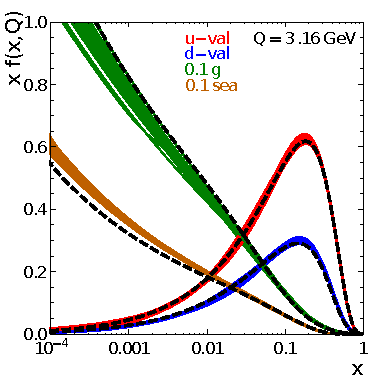
\includegraphics[width=0.5\textwidth]{CT10_1}}
   \subfloat[]{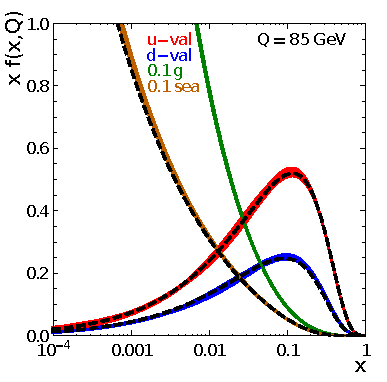
\includegraphics[width=0.5\textwidth]{CT10_2}}
   \caption[CT10 NNLO parton distribution functions.]{CT10 NNLO parton distribution functions for up and down quarks,
   gluons and sea quarks, given at two different factorisation scales: (a) Q = \SI{3.16}{\GeV}, (b) Q =
   \SI{85}{\GeV} \autocite{CT10_NNLO}.}
   \label{fig:CT10_PDFs}
\end{figure}

The total \ttbar production cross section for hard scattering processes in hadron collisions can be calculated to a
fixed order as \autocite{Sterman1986, primer_LHC}:
\begin{equation}
\sigma^{\ttbar} (s,\mtop^2) = \sum_{i,j} \int dx_i dx_j f_i(x_i, \mu_f^2) f_j(x_j,\mu_f^2) \hat{\sigma}_{i,j
\rightarrow \ttbar} (\hat{s}, \mtop^2, \alpha_S(\mu_r^2)),
\end{equation}
where the indices $i,j$ run over the incoming partons (gluons and quark-antiquark pairs), $x_{i,j}$ are the momentum
fractions of the incoming partons, $f_{i,j}$ are their parton distribution functions, and $\hat{\sigma}_{i,j
\rightarrow \ttbar}$ is the cross section of interacting partons, which depends on the parton centre of mass energy
$\hat{s} \sim x_i x_j s$, the top quark mass \mtop, and the QCD strong coupling constant $\alpha_S$. The latter
parameter is evaluated at renormalisation scale $\mu_r$. The top quark mass \mtop, as discussed in
Section~\ref{ss:top_mass}, also depends on the choice of renormalisation scheme and scale $\mu_r$.

The results of the most recent theoretical calculation of \ttbar cross section performed with
next-to-next-to-leading-order (NNLO) QCD corrections \autocite{NNLO_ttbar} are given in
Table~\ref{tab:ttbar_NNLO_xsections}. The cross section has also been measured by CMS and ATLAS experiments at the LHC
-- the comparison of these measurements with the theoretical prediction is shown in
Figure~\ref{fig:xsections_comparison_NNLO}.

\begin{table}[!hbp]
\centering
\caption{Theoretical predictions for \ttbar production cross section at
different LHC centre of mass energies, calculated at
next-to-next-to-leading-order (NNLO) \autocite{NNLO_ttbar}. The scales uncertainty corresponds to the choice of factorisation and renormalisation scales. }
\label{tab:ttbar_NNLO_xsections} 
\begin{tabular}{lrrr}
 \toprule
 $\sqrt{s}$ & $\sigma_\textrm{total}$ [\pb] & scales [\pb] & PDF [\pb] \\
 \midrule
 \SI{7}{\TeV}  & 172.0 & ${}^{+4.4~(2.6\%)}_{-5.8~(3.4\%)}$ & ${}^{+4.7~(2.7\%)}_{-4.8~(2.8\%)}$ \\
 \addlinespace[0.5em]
 \SI{8}{\TeV}  & 245.8 & ${}^{+6.2~(2.5\%)}_{-8.4~(3.4\%)}$ & ${}^{+6.2~(2.5\%)}_{-6.4~(2.6\%)}$ \\
 \addlinespace[0.5em]
 \SI{14}{\TeV} & 953.6 & ${}^{+22.7~(2.4\%)}_{-33.9~(3.6\%)}$ & ${}^{+16.2~(1.7\%)}_{-17.8~(1.9\%)}$ \\
 \bottomrule
\end{tabular}
\end{table}

\begin{figure}[bhtp]
   \centering
   {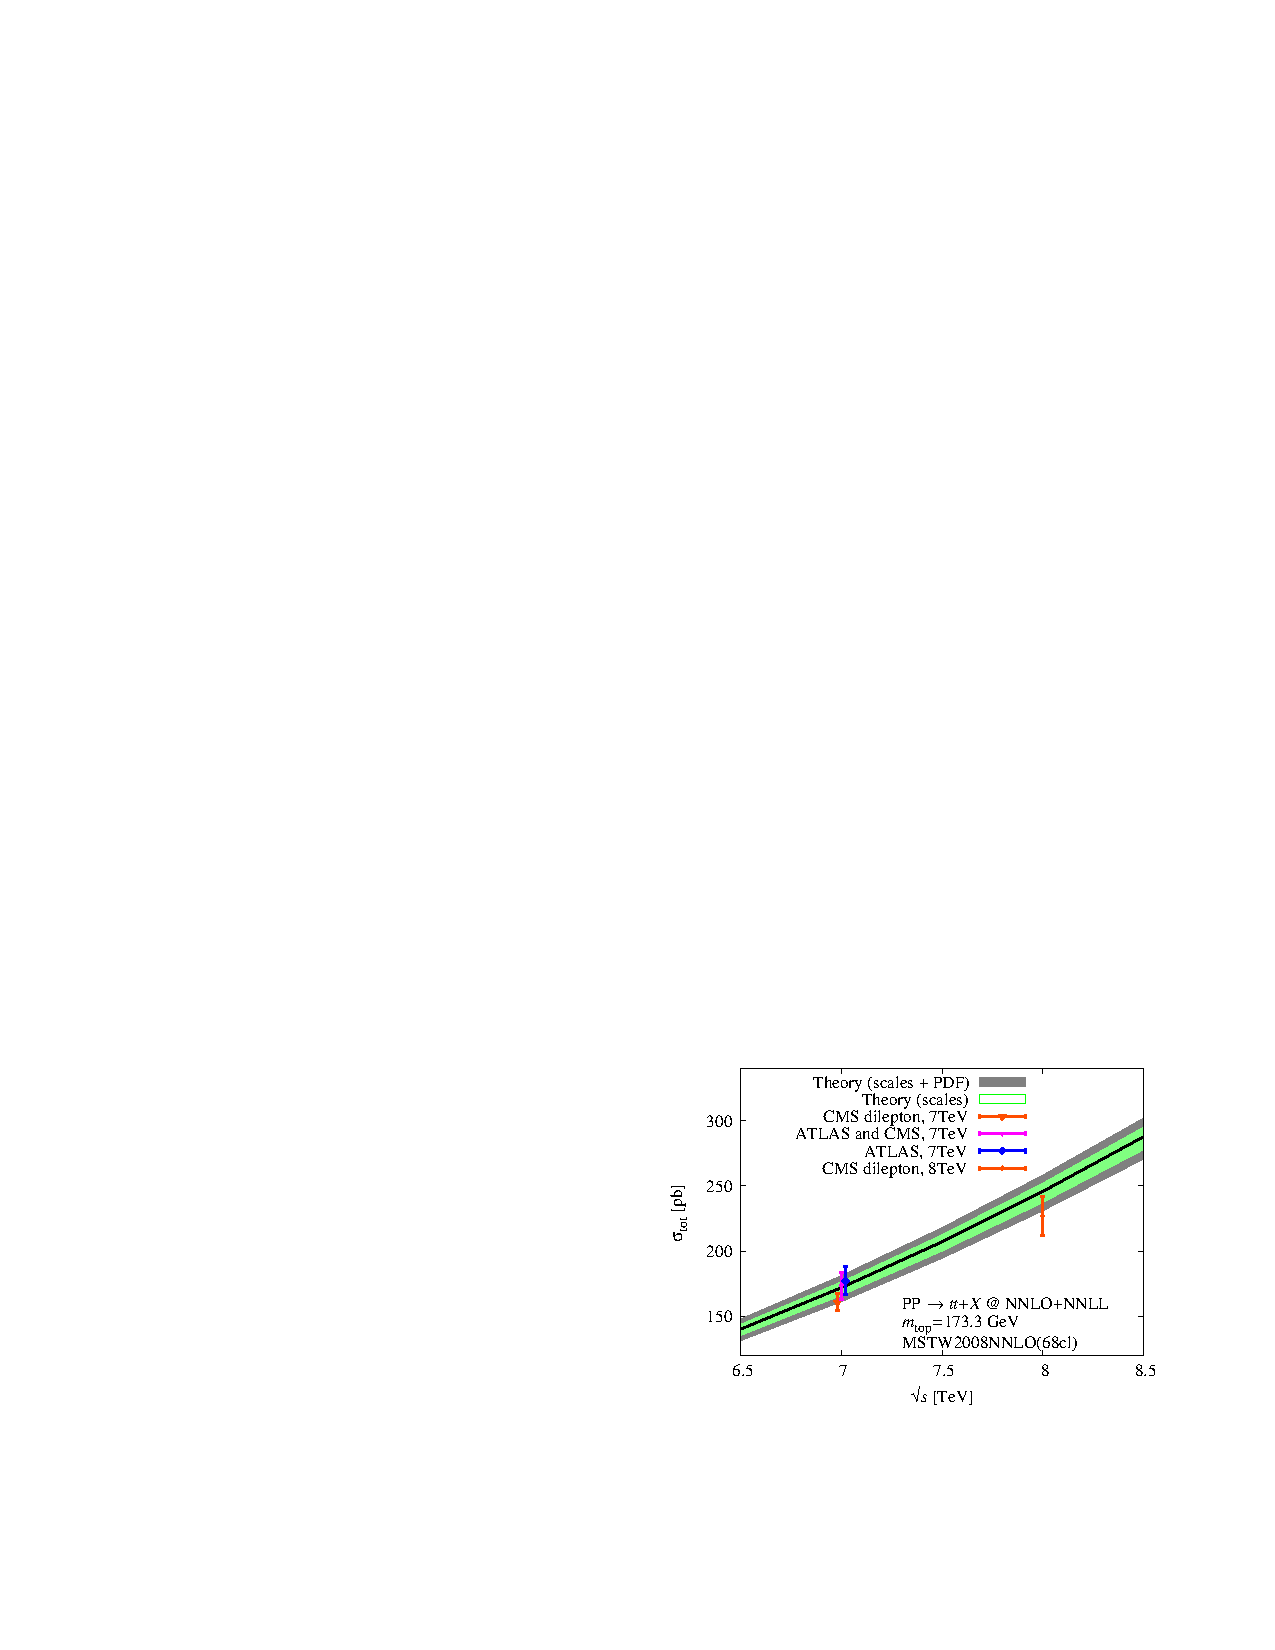
\includegraphics[width=0.7\textwidth]{xsections_comparison_NNLO}}
   \caption[Measurement of the \ttbar production cross section]{Measurement of the \ttbar production cross section at
   centre of mass energies of \SI{7}{\TeV} and \SI{8}{\TeV} by ATLAS and CMS experiments, compared with the theoretical
   prediction \autocite{NNLO_ttbar}.}
   \label{fig:xsections_comparison_NNLO}
\end{figure}

An abundance of top quark events at the LHC allows measurements of differential \ttbar production cross section with
respect to many different variables. These measurements provide important tools for validation of various MC models and
higher-order QCD calculations of \ttbar production. Since the very same models are used in BSM searches where \ttbar
events represent a major background, such validation is of great importance. Moreover, these measurements can themselves
be sensitive to signal contributions from new physics.

Normalised differential cross section in each bin $i$ of an observed variable $\mathrm{X}$ is given by:
\begin{equation}
\label{eq:normalised_differential_xsection_theory}
\frac{1}{\sigttbar^\mathrm{tot}} \frac{\mathrm{d}\sigma_i}{\mathrm{d} \mathrm{X}} = \frac{1}{\sigttbar^\mathrm{tot}}
\frac{x_i}{\Delta \mathrm{X}_i \calL},
\end{equation}
where $x_i$ is the number of signal events in data after subtraction of background, corrected for detector efficiency,
acceptance and migration between the bins of variable $\mathrm{X}$; $\calL$ is the total integrated luminosity; $\Delta
\mathrm{X}_i$ is the variable bin width; and $\sigttbar^\mathrm{tot}$ is the total \ttbar production cross section. The
normalisation is performed in order to cancel the systematic uncertainties that are correlated between the bins of
variable $\mathrm{X}$.

Both ATLAS and CMS collaborations have delivered a range of differential \ttbar production cross section measurements
\autocite{ATLAS_diff_xsections_7TeV, CMS_diff_xsections_7TeV}. For instance, Figure~\ref{fig:ATLAS_CMS_diff_xsections}
shows the normalised differential cross section with respect to the invariant mass of \ttbar pair ($m_{\ttbar}$),
measured by ATLAS and CMS collaborations using the $\sqrt{s} = \SI{7}{\TeV}$ LHC data. These measurements require a full
kinematic reconstruction of the semileptonic \ttbar decay in order to accurately calculate the $m_{\ttbar}$ variable.
Other variables requiring the kinematic reconstruction include the transverse momenta of top quarks decaying either
leptonically or hadronically, their rapidities, etc.

\begin{figure}[hbtp]
   \centering
   \subfloat[]{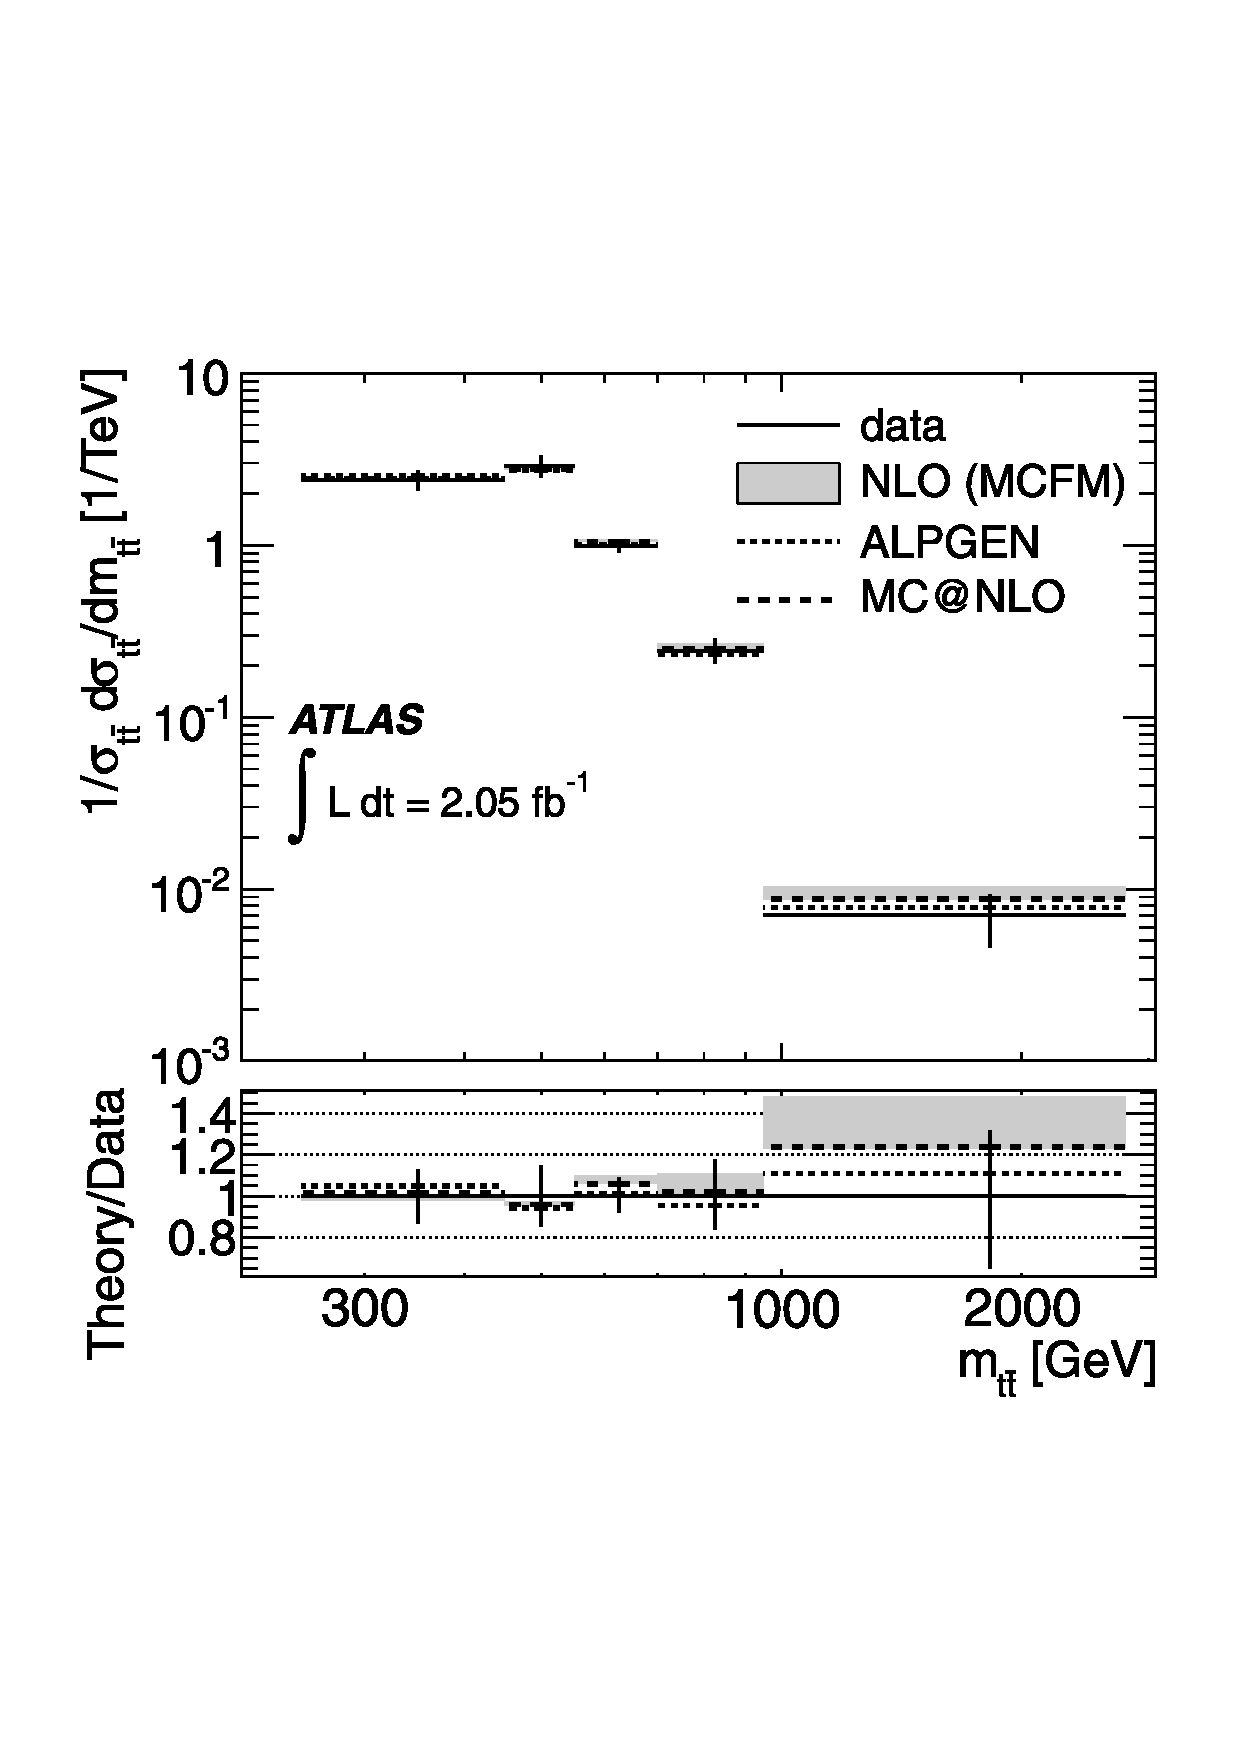
\includegraphics[width=0.5\textwidth]{ATLAS_diff_xsection_mtt}}
   \subfloat[]{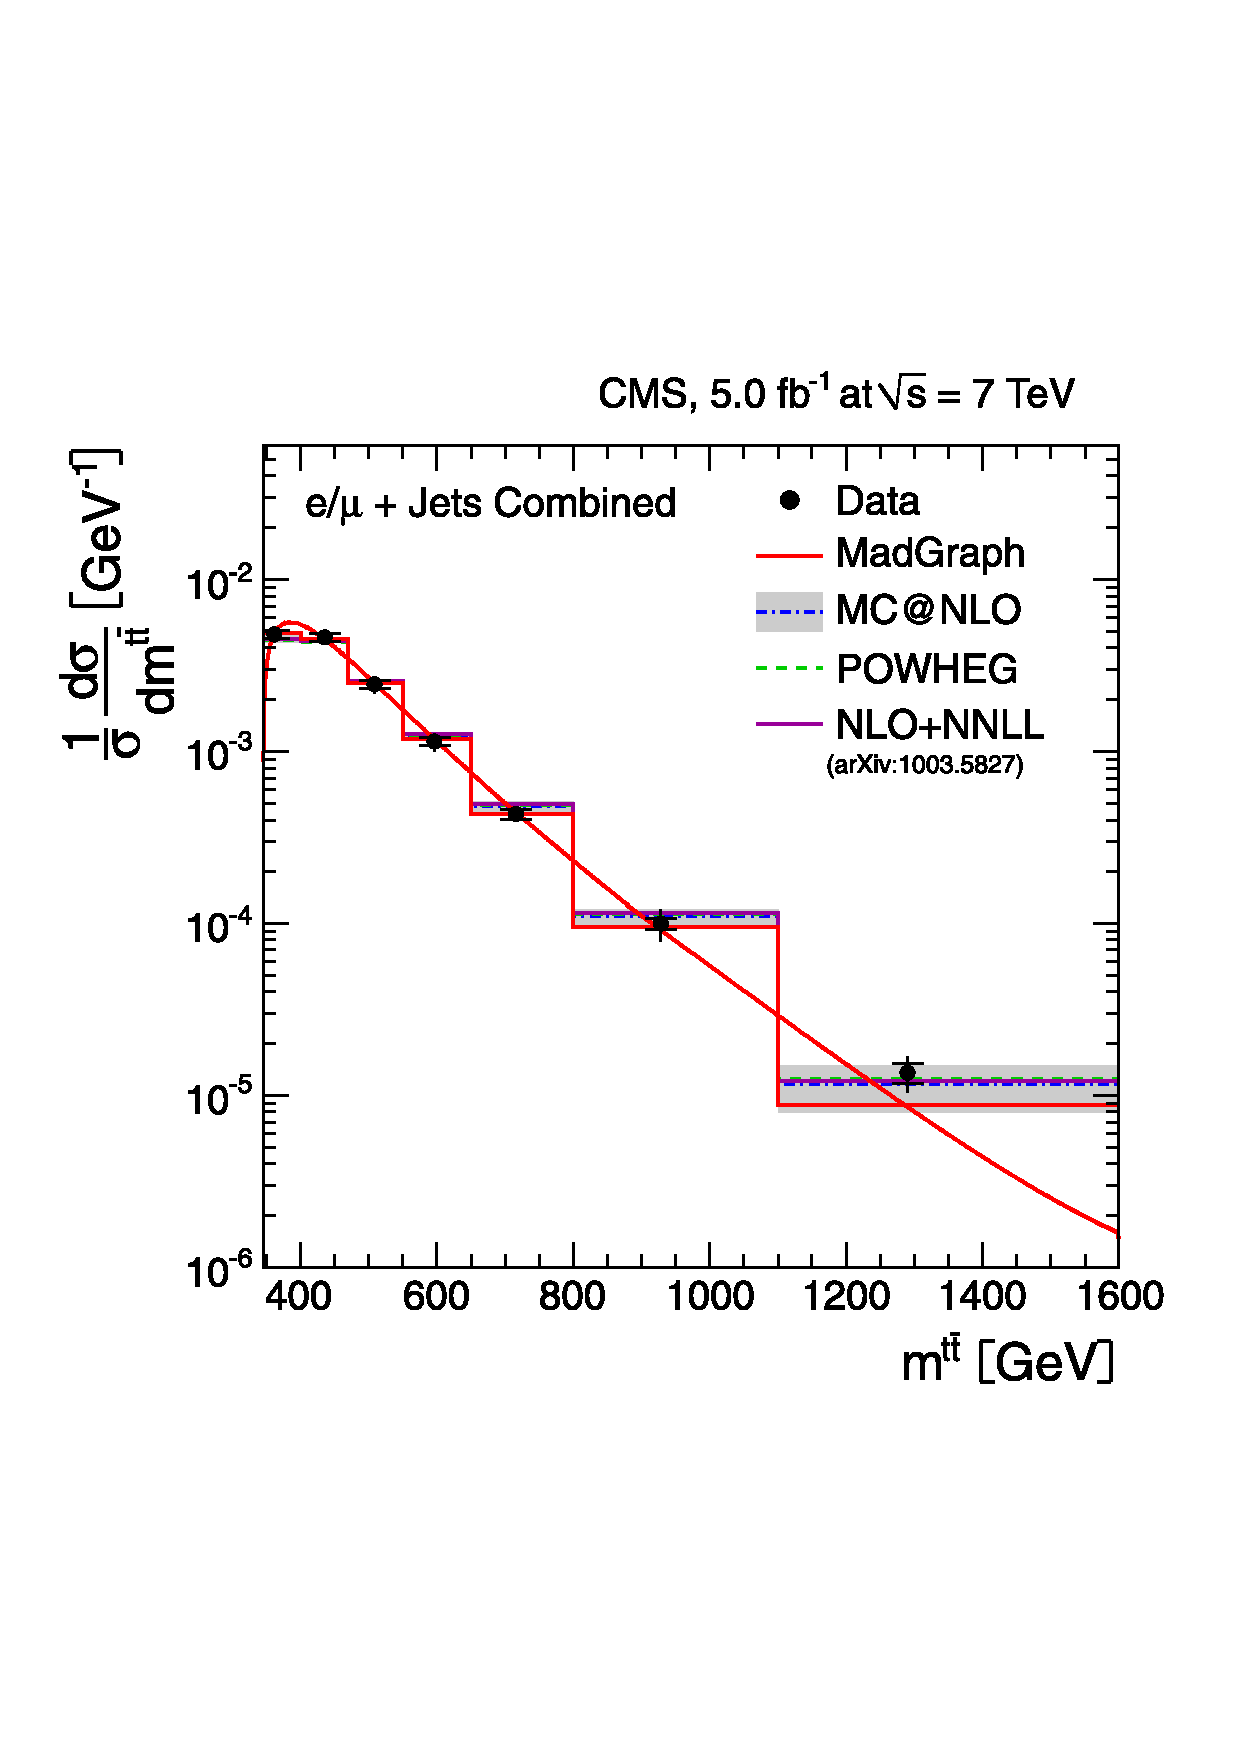
\includegraphics[width=0.5\textwidth]{CMS_diff_xsection_mtt}}
   \caption[Normalised differential \ttbar production cross section measurements by ATLAS and CMS
   collaborations]{Normalised differential \ttbar production cross section measurements in the $l+$jets channel with
   respect to the invariant mass of a top quark pair. (a) ATLAS measurement \autocite{ATLAS_diff_xsections_7TeV}, (b)
   CMS measurement \autocite{CMS_diff_xsections_7TeV}.}
   \label{fig:ATLAS_CMS_diff_xsections}
\end{figure}

In this thesis, the \ttbar differential cross section is measured with respect to so-called event-level (or global)
variables, not requiring a kinematic reconstruction of the \ttbar decay -- for example, missing transverse energy (\MET)
or total hadronic activity (\HT) in the event (see Section~\ref{ss_xsection:variables}). The main advantage of these
measurements is the absence of the systematic uncertainty associated with the kinematic reconstruction. Additionally,
signs of new physics scenarios could be revealed in the tails of these distributions. For example, an associative
production of a \ttbar pair with some new resonance ($\ttbar+\mathrm{X}$) decaying invisibly can show up in the tail of
the missing transverse energy distribution.

\section{Summary}
In this chapter, an overview of the Standard Model has been presented. The concept of gauge principle and its
applications in the electroweak theory and the Quantum Chromodynamics, as well as the mechanism of the electroweak
symmetry breaking have been briefly described. Shortcomings of the Standard Model and some models proposing the
solutions have been mentioned. Finally, an introduction to the top quark physics has been given, with pointing out the
relevance and importance of the top quark mass and differential cross section measurements presented in this thesis.

%%% Local Variables: 
%%% mode: latex
%%% TeX-master: "../thesis"
%%% End: 

%!TEX root = ../thesis.tex

\chapter{The LHC and the CMS detector}
\label{c:detector}
\ifpdf
    \graphicspath{{03_Detector/plots/}}
\else
    \graphicspath{{03_Detector/plots/EPS/}{03_Detector/plots/}}
\fi

\section{The Large Hadron Collider}
\label{s:LHC}

The LHC \autocite{LHC} is currently the largest and the most powerful particle accelerator ever built. It is installed
in the \SI{26.7}{\km} tunnel that was originally constructed for the LEP accelerator in the 1980s. The tunnel lies at a
depth of \SIrange{45}{170}{\metre} underground between the Jura mountain and Lake Geneva, being the main part of the
CERN accelerator complex.

The machine is designed to accelerate proton beams and provide collisions at a centre of mass energy of $\sqrt s =$
\SI{14}{\TeV}. Unlike particle-antiparticle colliders, the LHC requires two rings with opposite magnetic dipole fields
in order to maintain and collide two counter-rotating proton beams. Since the tunnel was originally designed for the
electron-positron LEP, it has an internal diameter of \SI{3.7}{\metre} which is not enough to install two separate
independent rings. Therefore, a twin-bore magnet design was adopted \autocite{Blewett}, which resulted in substantial
cost savings.

\begin{figure}[!htbp]
  \begin{center}
    \leavevmode
    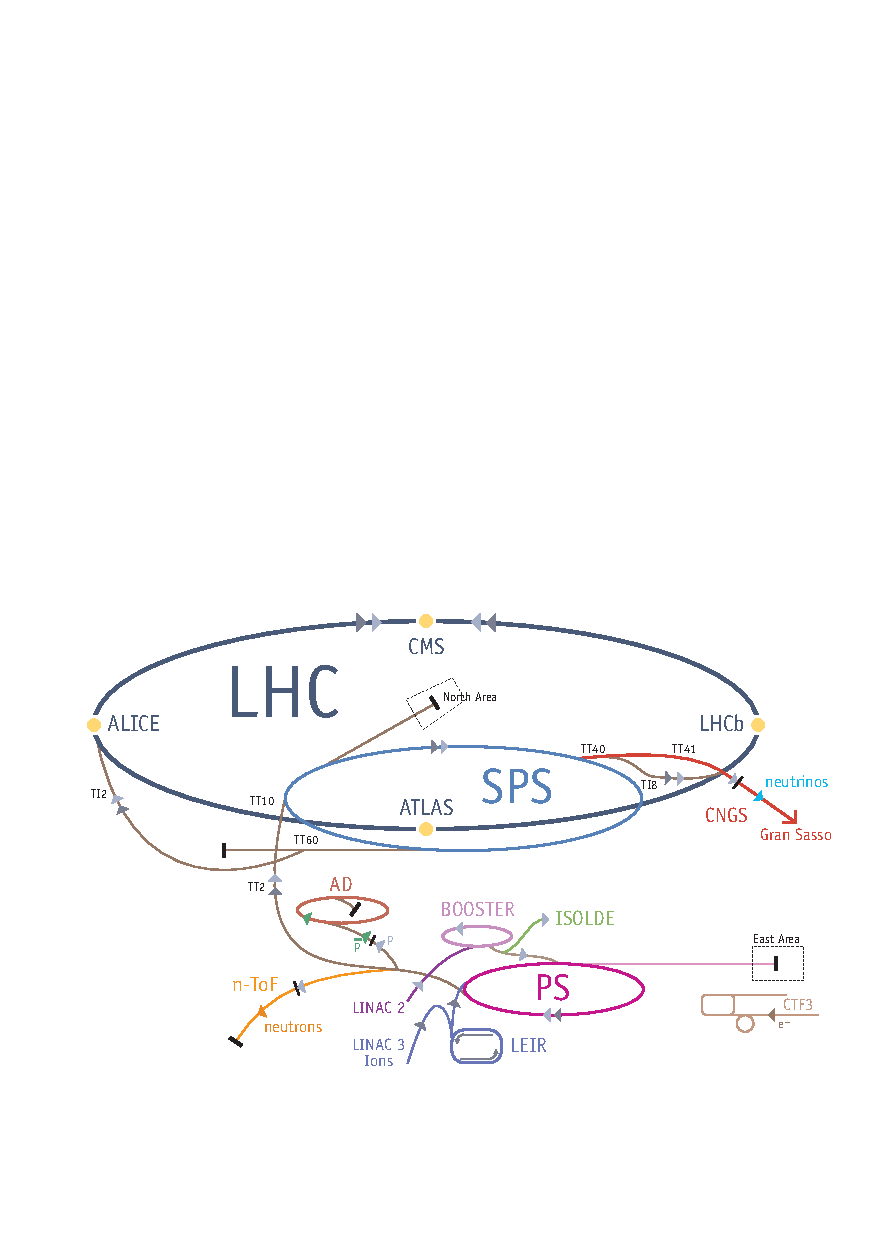
\includegraphics[width=\columnwidth]{LHC}
    \caption{CERN accelerator complex.}
    \label{LHC}
  \end{center}
\end{figure}

A schematic view of the LHC accelerator chain is shown in Figure~\ref{LHC}. Initially, the protons are obtained by
stripping orbiting electrons from hydrogen atoms. Then they are injected into the linear accelerator LINAC2 to reach the
energy of \SI{50}{\MeV} and enter the Proton Synchrotron Booster (PSB). The booster accelerates them to \SI{1.4}{\GeV}
and passes the beam to the Proton Synchrotron (PS) where the energy rises to \SI{25}{\GeV}. In the next step, protons
enter the Super Proton Synchrotron (SPS) where they are accelerated to \SI{450}{\GeV}. Finally, the beam is transferred
to the LHC in both clockwise and anti-clockwise directions where it takes about 20 minutes to reach the design
\SI{7}{\TeV} energy (per beam).

\textit{[add the number of magnets, total energy stored, number of bunches, bunch spacing etc.?]}

The LHC has four interaction points, providing collisions to four major experiments. Two of them, CMS and ATLAS, are
multi-purpose high-luminosity experiments with a peak luminosity of $L = $ \SI{d34}{\cm^{-2} s^{-1}}. The other two
experiments operate at low luminosities and have more specific physics goals: LHCb studies b-meson decays, and Alice is
a dedicated heavy ion experiment.

The instantaneous luminosity of a collider can be calculated as
\begin{equation}
	L = \frac{n_1 n_2 f}{4 \pi \sigma_x \sigma_y},
\end{equation}
where $n_1$ and $n_2$ are the numbers of particles in each of the colliding bunches, $f$ is the revolution frequency,
$\sigma_x$ and $\sigma_y$ are the horizontal and vertical beam sizes, assuming the two beams have the same size.

The number of events generated in the collisions per second is given by
\begin{equation}
	N_{events} = L \times \sigma,
\end{equation}

where $\sigma$ is the cross section of the process under study.

\textit{[add the plots with cross sections and production rates?]}

The LHC started operating on the 10th of September 2008, with the first beams fully circulating in both rings. However,
only 9 days later a magnet quench occurred in two sectors of the tunnel, which was caused by an electrical fault due to
a bad connection between two magnets. A consequent liquid helium explosion damaged a total of 53 superconducting
magnets. Over a year was spent on repairs and tests, and the first collisions were recorded on the 23rd of November 2009
at a centre of mass energy of \SI{0.9}{\TeV}. The following few months showed the continuous ramp up of the beam
energies up to \SI{3.5}{\TeV} per beam which was achieved on the 30rd of March 2010 when the LHC physics programme
started.

Throughout the rest of 2010, the two general-purpose LHC experiments (CMS and ATLAS) recorded approximately
\SI{40}{\invpb} of data, which resulted in the first measurements of various physics processes at the LHC. The following
year became the main \SI{7}{\TeV} data-taking period, with about \SI{5}{\invfb} of data recorded by ATLAS and CMS. On
the 5th of April 2012 the centre of mass energy was increased to 8 TeV, and July of 2012 marked the first major
discovery of a new boson which was later shown to be consistent with the Standard Model Higgs boson, according to
approximately \SI{21.8}{\invfb} of data recorded until early 2013. A long shut-down is planned for the following two
years with various upgrades scheduled. The next physics run is expected in 2015 with the beam energy increased up to 6
or \SI{7}{\TeV}.

\textit{[add any upgrade details and distant future plans, like SLHC?]}

\section{The CMS Detector}
\label{s:CMS}

The Compact Muon Solenoid \autocite{CMS} is a general-purpose detector designed to carry out precise measurements of the
Standard Model and searches for physics beyond it. The primary design requirement was the ability to discover the nature
of electroweak symmetry breaking, and the first observation of a Higgs boson was obtained in the Summer of 2012
\autocite{CMS_Higgs}.

The detector is installed at one of the LHC interaction points (Point 5) at about \SI{100}{\metre} underground near the
French village of Cessy, between the Jura mountains and Lake Geneva. The overall dimensions of the CMS detector are a
length of \SI{21.6}{\metre}, a diameter of \SI{14.6}{\metre} and a total weight of \SI{12500}{\tonne}.

\begin{figure}[htbp]
  \begin{center}
    \leavevmode
    \includegraphics[width=\columnwidth]{CMS}
    \caption{Sectional view of the CMS detector.}
    \label{CMS}
  \end{center}
\end{figure}

The sectional view of CMS is shown in Figure~\ref{CMS}. In the centre of the detector, tracking and calorimetry systems
are surrounded by the superconducting solenoid. On the outermost part of it the magnetic flux is returned through the
iron yoke in which the muon system is also integrated. All the sub-systems are discussed in the following sections in
more detail.

The cylindrical shape of the CMS detector dictates using a cylindrical coordinate system, with the origin centred at the
interaction point, the $x$-axis pointing towards the centre of the LHC ring, the $y$-axis pointing upwards and the
$z$-axis pointing along the beamline in the anti-clockwise direction. The azimuthal angle $\phi$ is measured from the
$x$-axis in the transverse ($x-y$) plane and the polar angle $\theta$ is measured from the $z$-axis. The radial distance
to the beamline is denoted by $r$. Pseudorapidity is defined as:
\begin{equation}
  \eta = - \ln{\tan{\frac{\theta}{2}}}.
\end{equation}
This implies that the particles moving in the transverse plane (perpendicular to the beamline) have a pseudorapidity of
0, whereas the beam direction has an infinite pseudorapidity. Considering the cylindrical shape of the detector, it has
barrel and endcap regions, with the transition occurring at $\eta \sim 1.4$. The momentum and energy transverse to the
beamline are denoted by $p_T$ and $E_T$ respectively; the imbalance of the energy measured in the transverse plane,
called missing transverse energy, is denoted by \ETm.

\subsection{Inner Tracking System}
\label{ss:tracker}
The tracking system lies in the heart of the CMS detector and is the closest to the interaction point where the particle
flux has the highest value. This imposes demanding requirements on the configuration of the system. At design luminosity
of $L = $ \SI{d34}{\cm^{-2} s^{-1}} with the bunch spacing of \SI{25}{\ns}, an average of \num{1000} particles from
about \num{25} proton-proton interactions (pile-up vertices) is expected to traverse the tracker for each bunch
crossing. However, up until the long shutdown a bunch spacing of \SI{50}{\ns} was used, which meant a higher number of
protons in each bunch leading to approximately twice the number of pile-up vertices. Therefore, in order for the
particle tracks to be identified reliably and separately for each bunch crossing, the tracker requires very fine
granularity and fast response parameters. Another complication caused by the intense particle flux is the severe
radiation damage, so the tracker has to be highly resilient in operating in the harsh environment for a reasonable
lifetime.

To meet these requirements on granularity, response time and radiation resilience, the tracker design was chosen to be
based on silicon detector technology. Although capable of meeting such conditions, this technology has a disadvantage of
a high power density of on-detector electronics. This implies the necessity of an efficient cooling system. Moreover, a
large amount of dense material interacting with the particles leads to higher multiple scattering, bremsstrahlung,
photon conversions and nuclear interactions. Therefore, there are complications in the reconstruction of the tracks,
meaning some loss of efficiency and precision. This will be discussed in detail later on in the object reconstruction
section.

\begin{figure}[htbp]
  \begin{center}
    \leavevmode
    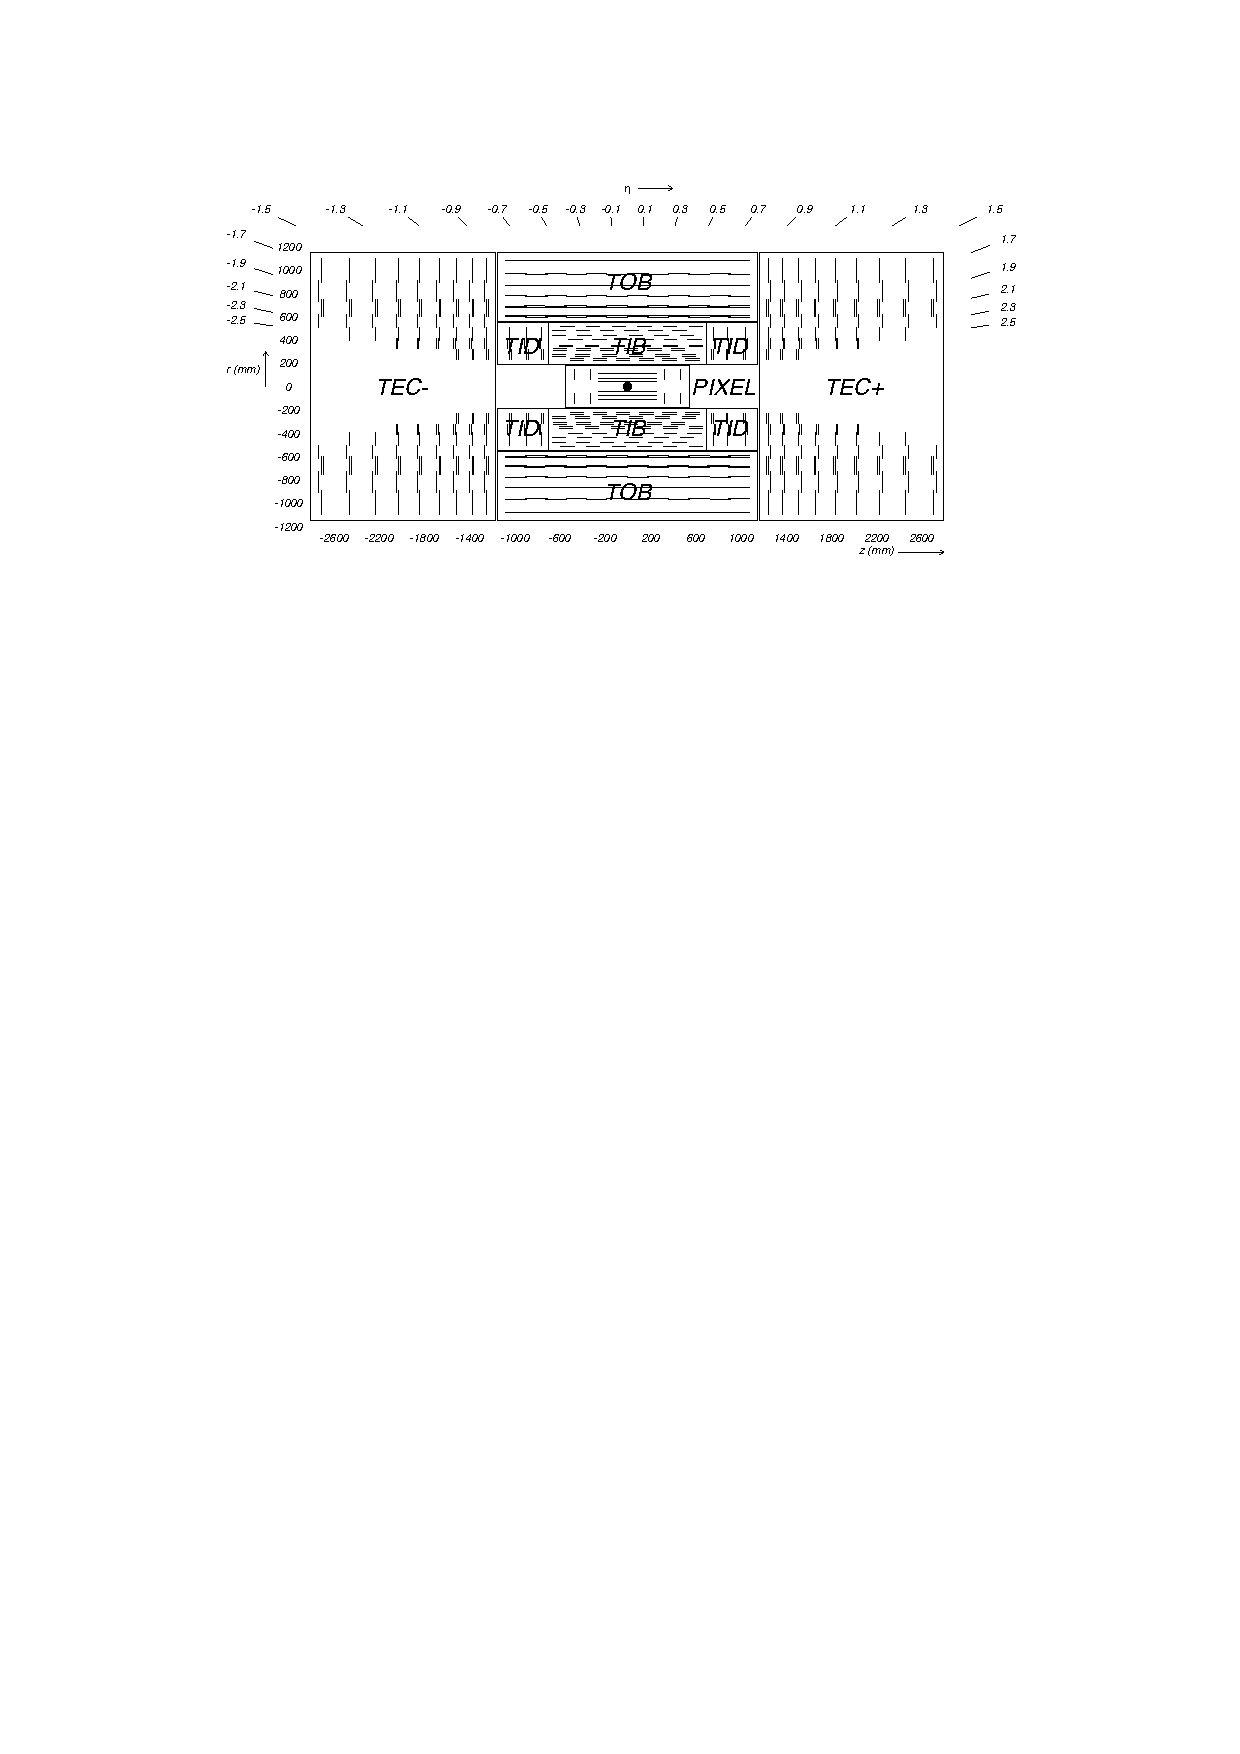
\includegraphics[width=\columnwidth]{tracker}
    \caption{Cross-section of the CMS tracker system \autocite{CMS}.}
    \label{Tracker}
  \end{center}
\end{figure}

Figure~\ref{Tracker} shows the overall layout of the tracking system. It consists of the inner pixel detector, located
in the vicinity of the interaction point, and silicon strip tracker detectors: inner barrel and disks (TIB and TID),
outer barrel (TOB) and endcaps (TEC). The geometrical acceptance of the tracker system goes up to \abs\eta \num{<2.5}.
The outer radius of the CMS tracker reaches approximately \SI{110}{\cm}, and its total length is about \SI{540}{\cm}.

The pixel detector consists of three layers of pixel sensors at radii of \SIlist{4.4;7.3;10.2}{\cm} from the beamline in
the barrel region. In addition there are two endcap disks on each side at \abs z $=$ \SIlist{34.5;46.5}{\cm}. The pixel
size equals \num{100x150} \si{\micron\squared} in $r \phi \times z$ coordinates. The pixel detector has 66 million
pixels and the total area of about \SI{1}{\m\squared}.

The silicon strip tracker consists of several layers of silicon microstrip detectors. It covers the region between
\SIrange{20}{110}{\cm} in radius and extends up to \SI{+-280}{\cm} in the z direction. The Tracker Inner Barrel (TIB) is
made out of 4 layers and the Tracker Outer Barrel (TOB) has 6 layers in it. The tracker endcaps (TEC) comprise 9 disks,
and there are also the tracker inner disks (TID) that consist of 3 disks filling the gap between TIB and TEC as shown in
Figure~\ref{Tracker}. There are \num{9.3} million silicon strips covering the area of about \SI{200}{\m\squared}. The
silicon sensors' thickness varies between \num{320} and \SI{500}{\micron} and the strip pitch varies from
\SI{80}{\micron} in the TIB to \SI{180}{\micron} in TOB and TEC.

\begin{figure}[!htbp]
  \begin{center}
    \leavevmode
    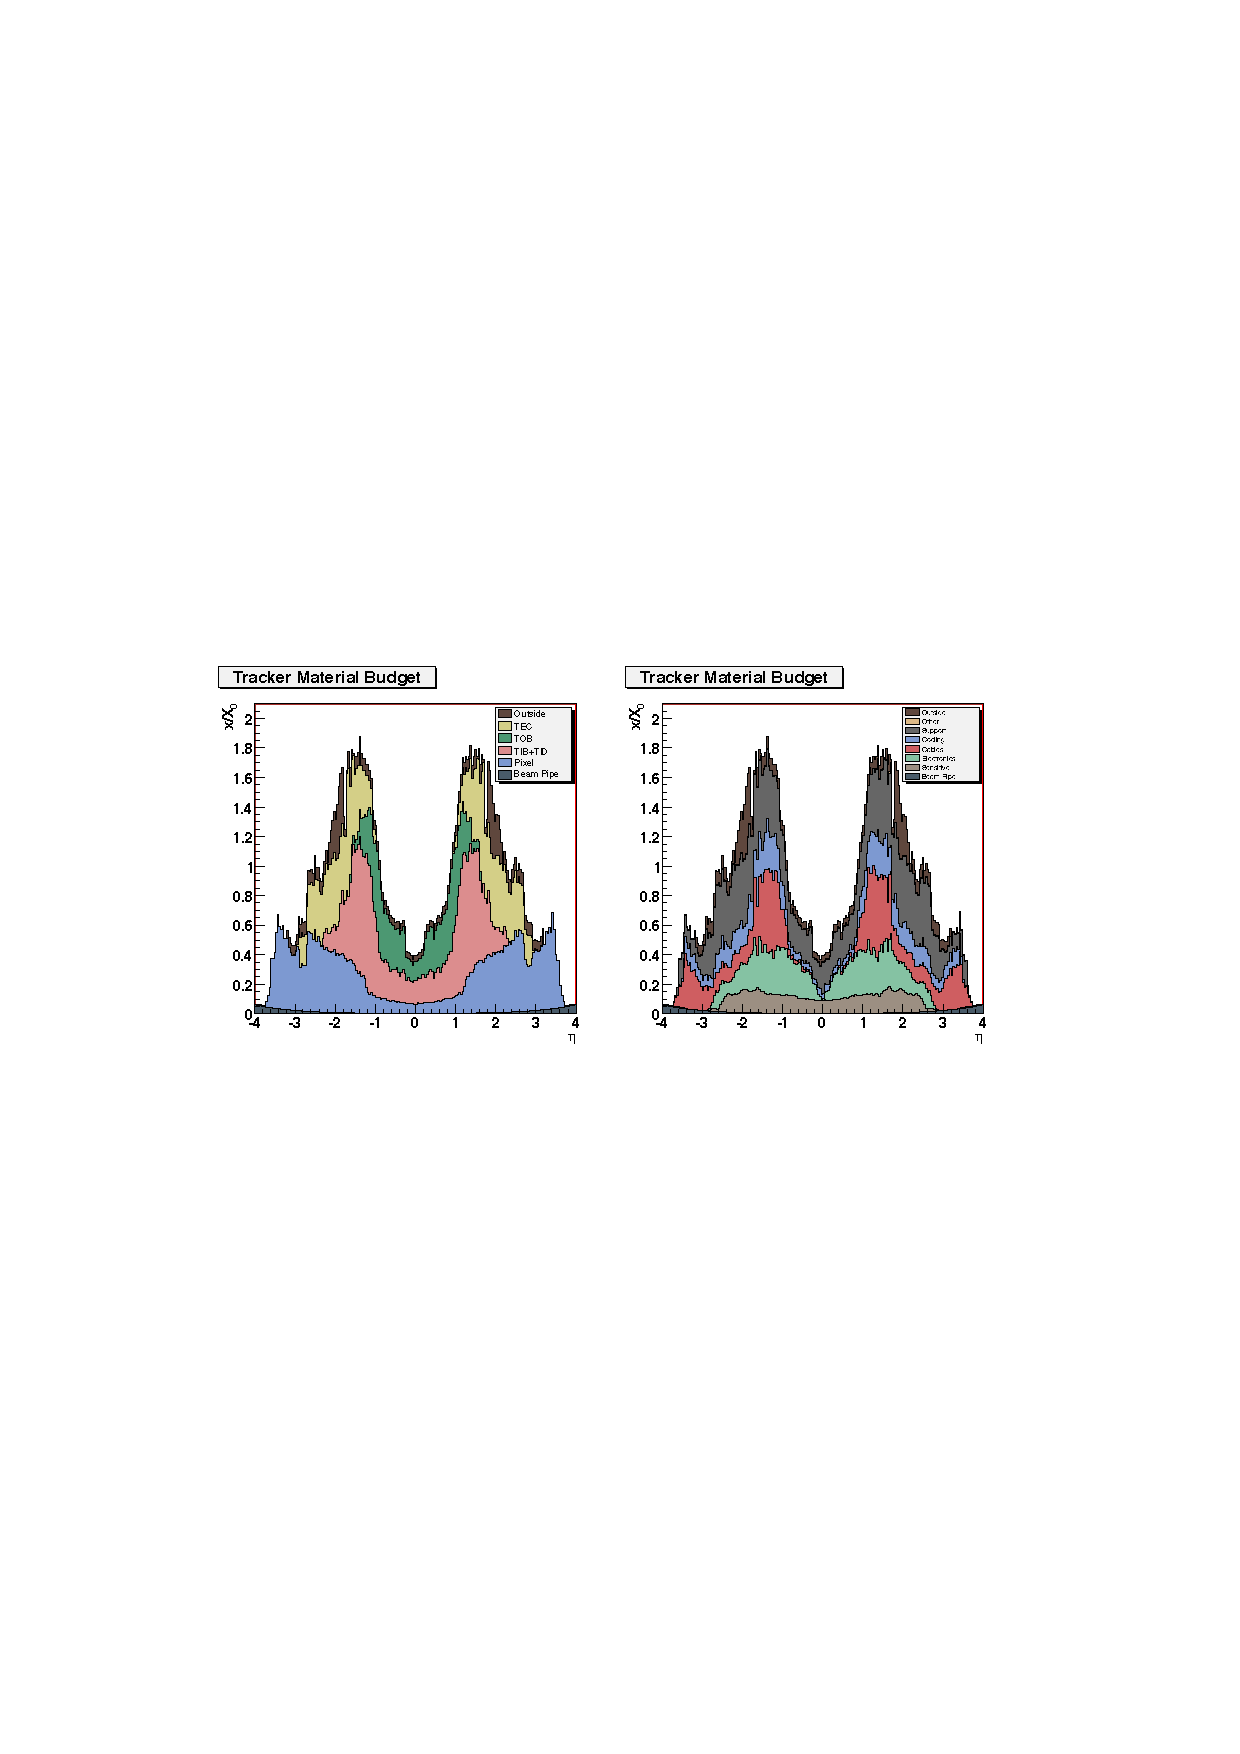
\includegraphics[width=\columnwidth]{tracker_material_budget}
    \caption{Material budget as a function of pseudorapidity $\eta$ for the different sub-detectors of the tracker
    (left) and broken down into the functional contributions (right), in units of radiation length \autocite{CMS}.}
    \label{tracker_material_budget}
  \end{center}
\end{figure}

%update with http://cms.cern.ch/iCMS/jsp/analysis/admin/analysismanagement.jsp?awg=TRK&dataset=All&awgyear=2011

The silicon detectors of the tracker, the readout electronics and support structure form a considerable amount of
material for the particles traversing from the interaction point. Figure~\ref{tracker_material_budget} \autocite{CMS}
shows the material budget of the CMS tracker in units of radiation lengths\footnote{A material's radiation length is the
mean distance over which a high-energy electron loses all but $1/e$ of its energy by bremsstrahlung; this is equal to
\num{7/9} of the mean free path for pair production by a high-energy photon.} ($X_0$). It grows from about \num{0.4}
$X_0$ to \num{1.8} $X_0$ in the barrel region, and then decreases to about \num{1} $X_0$ in the endcaps. This causes a
substantial conversion rate for photons and electrons in the tracker material; it also will be discussed in more detail
in the electron reconstruction section.

\textit{[perhaps need to add the $p_T$ resolution plots]}

\subsection{Electromagnetic Calorimeter}
The next detector subsystem which is surrounding the tracker is the electromagnetic calorimeter, or ECAL. It is of a
primary importance for the analyses described in this thesis, as it provides information for the electron and positron
reconstruction. Combination of this information with that from the tracking system must ensure a precise measurement of
electron position and momentum, and also sufficient background removal. It has to effectively distinguish the energy
deposit shape of an electromagnetic particle from the one of a hadronic particle, which requires good segmentation and
high resolution.

ECAL is a hermetic, high-granularity, high-resolution scintillating crystal calorimeter consisting of \num{61200} lead
tungstate ($\textrm{PbWO}_4$) crystals located in the central barrel region (\abs\eta $<1.479$), and \num{7324} crystals
in each of the two endcaps (\num{1.479} $<$\abs\eta\num{<3.0}). All crystals are followed by photodetectors reading and
amplifying their scintillation: avalanche photodiodes (APD) are used in the barrel, and vacuum phototriodes (VPTs) are
used in the endcaps. These different choices were caused by the configuration of the magnetic field and the expected
level of radiation.

\begin{figure}[!htbp]
  \begin{center}
    \leavevmode
    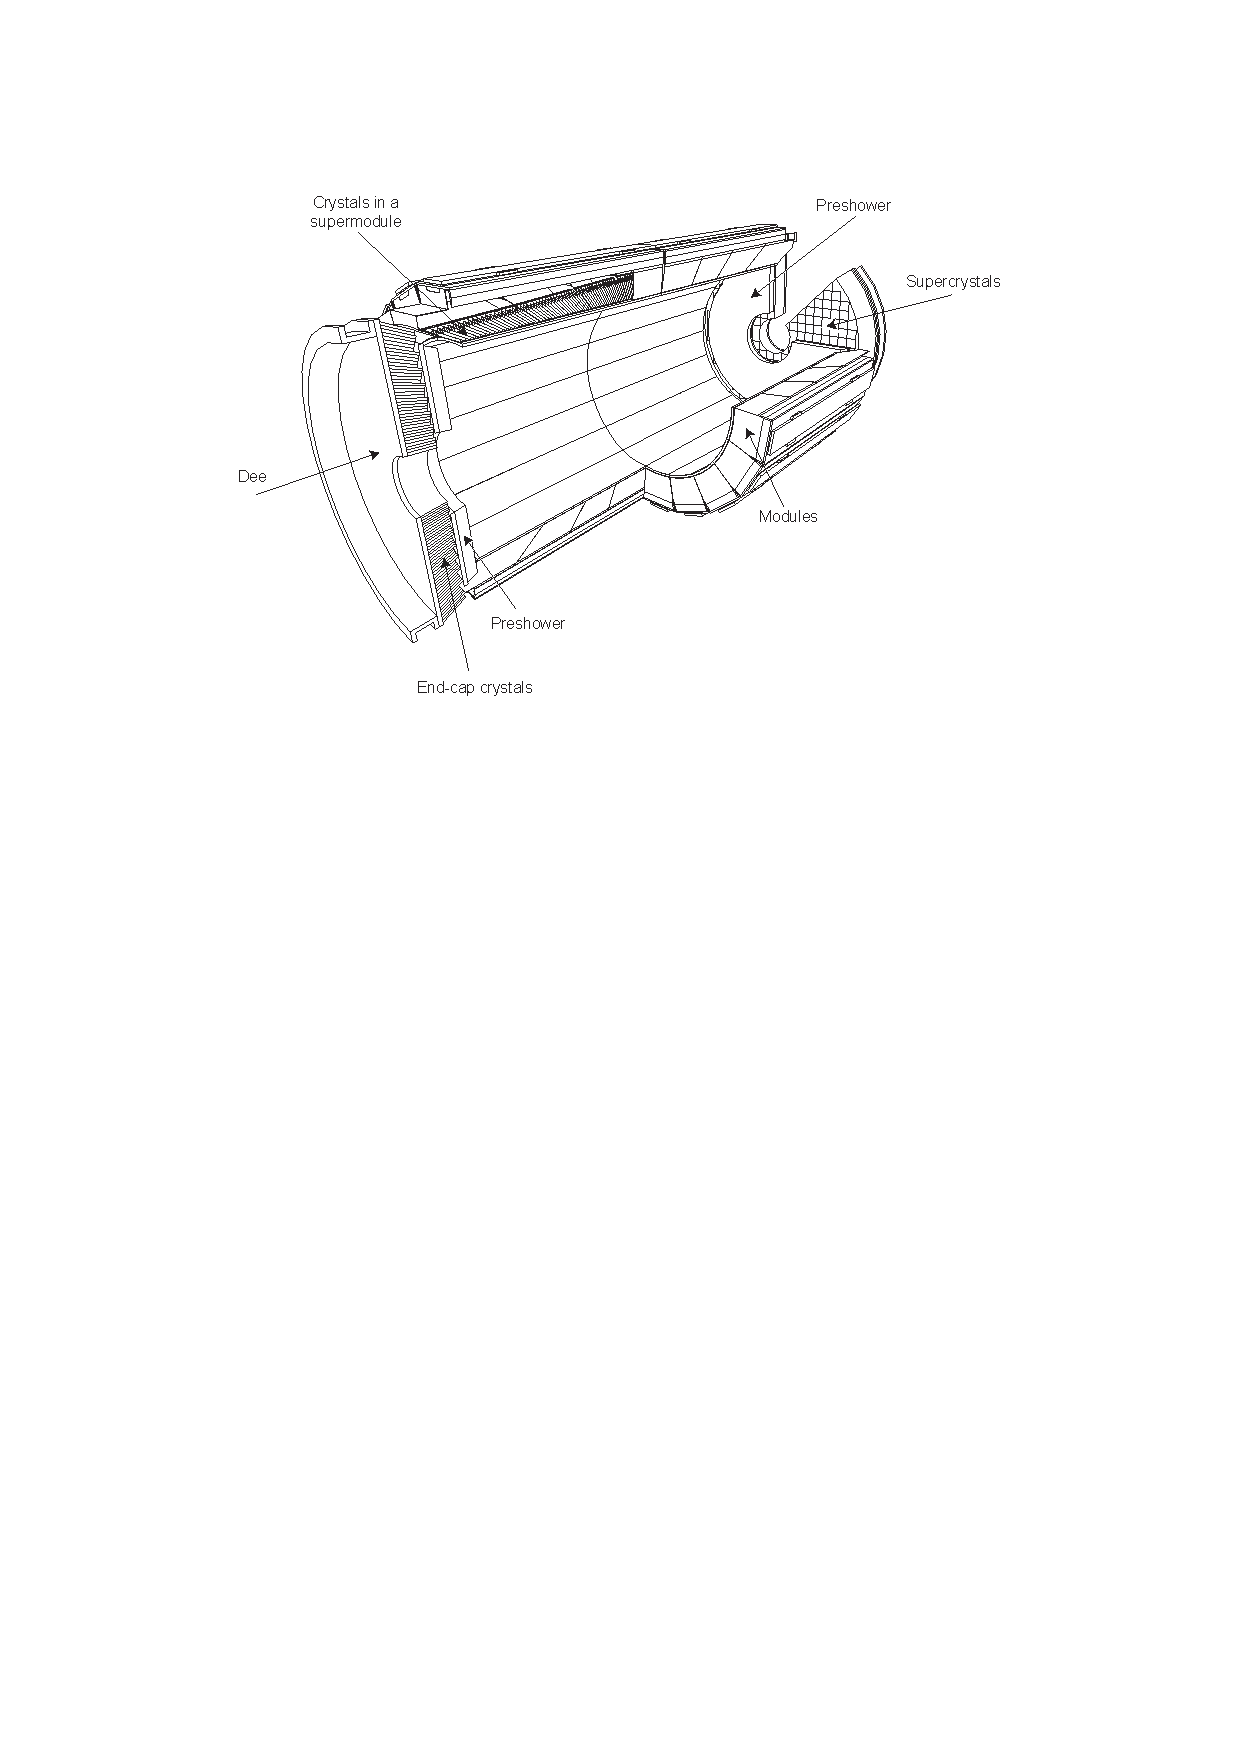
\includegraphics[width=\columnwidth]{ECAL}
    \caption{Layout of the CMS electromagnetic calorimeter \autocite{CMS}.}
    \label{ECAL}
  \end{center}
\end{figure}

The layout of the ECAL sub-detector is shown in Figure~\ref{ECAL}. An additional preshower detector is used in the
endcap region to lower the required detector depth. Its principal aim is to identify neutral pions in the endcaps, but
it also helps to distinguish neutral pions and electrons from minimum ionising particles and improves the position
determination of electrons and photons with high granularity.

\begin{table}[htbp]
\caption{ECAL crystal characteristics}
\label{ECAL_crystals}
\begin{center}
\begin{tabular}{|l|l|l|}
  \hline             
   & Barrel & Endcaps \\
  \hline
  number of crystals & \num{61200} & \num{14648} \\
  crystal cross-section in ($\eta$, $\phi$) & \num{0.0174 x 0.0174} & varies \\
  crystal cross-section at the front & \num{22x22} \si{\mm\squared} & \num{28.62x28.62} \si{\mm\squared} \\
  crystal cross-section at the rear & \num{26x26} \si{\mm\squared} & \num{30x30} \si{\mm\squared} \\
  crystal length & \SI{230}{\mm} (\num{25.8}$X_0$) & \SI{220}{\mm} (\num{24.7}$X_0$) \\
  \hline  
\end{tabular}
\end{center}
\end{table}

The main geometrical characteristics of the ECAL crystals are shown in Table~\ref{ECAL_crystals}. The choice of lead
tungstate was driven by the constraints of the CMS design. It is a very dense material (\SI{8.28}{g\per\cm\cubed}) with
a short radiation length of $X_0 = \SI{0.89}{\cm}$, which allows the calorimeter to fit inside the compact magnet. Lead
tungstate also has a small Moli\`ere radius\footnote{The Moli\`ere radius $R_\mu$ is a characteristic constant of a
material giving the scale of the transverse dimension of the fully contained electromagnetic showers initiated by an
incident high energy electron or photon. It is defined as the radius of a cylinder containing an average of
\SI{90}{\percent} of the shower's energy deposition.} of \SI{2.2}{\cm}, which allows a calorimeter with fine
granularity. Finally, the crystals emit \SI{80}{\percent} of their scintillation light in just \SI{25}{\ns}, however the
light yield is relatively low. At \SI{18}{\degreeCelsius}, about \num{4.5} photoelectrons per MeV are collected. The
dependence of the light yield on temperature requires a cooling system capable of keeping the crystal temperature stable
within \SI{+-0.05}{\degreeCelsius} to preserve energy resolution \autocite{CMS_TDR1}.

\begin{figure}[htbp]
  \begin{center}
    \leavevmode
    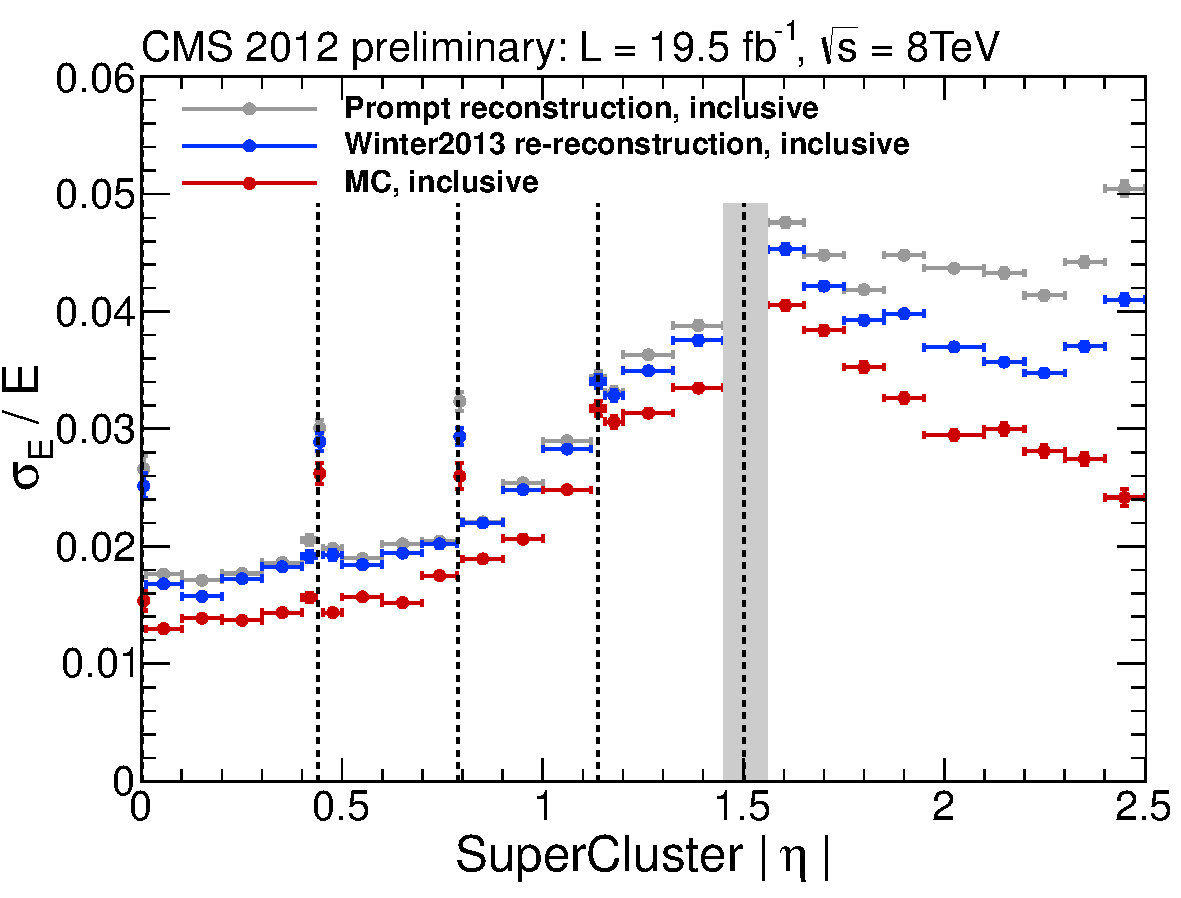
\includegraphics[width=0.7\columnwidth]{ECAL_resolution}
    \caption{ECAL energy resolution derived from the test beam measurements as a function of deposited energy. The
    stochastic, noise, and constant contributions are shown \autocite{CMS}.}
    \label{ECAL_resolution}
  \end{center}
\end{figure}

The energy-dependent resolution of the calorimeter can be parameterised as follows \autocite{CMS}:
\begin{equation}
  \left(\frac{\sigma}{E}\right)^2 = \left(\frac{S}{\sqrt E}\right)^2 + \left(\frac{N}{E}\right)^2 + C^2.
\end{equation}
where $S$ is the stochastic term, $N$ is the noise term, and $C$ is the constant term. Figure~\ref{ECAL_resolution}
shows the energy resolution measured using incident electrons, during the beam tests in 2004.

\subsection{Hadron Calorimeter}

The hadron calorimeter (HCAL) is the next sub-detector located mostly inside the solenoid and completing the CMS
calorimetry system. It is essential for the measurement of hadron jets and missing transverse energy.

\begin{figure}[htbp]
  \begin{center}
    \leavevmode
    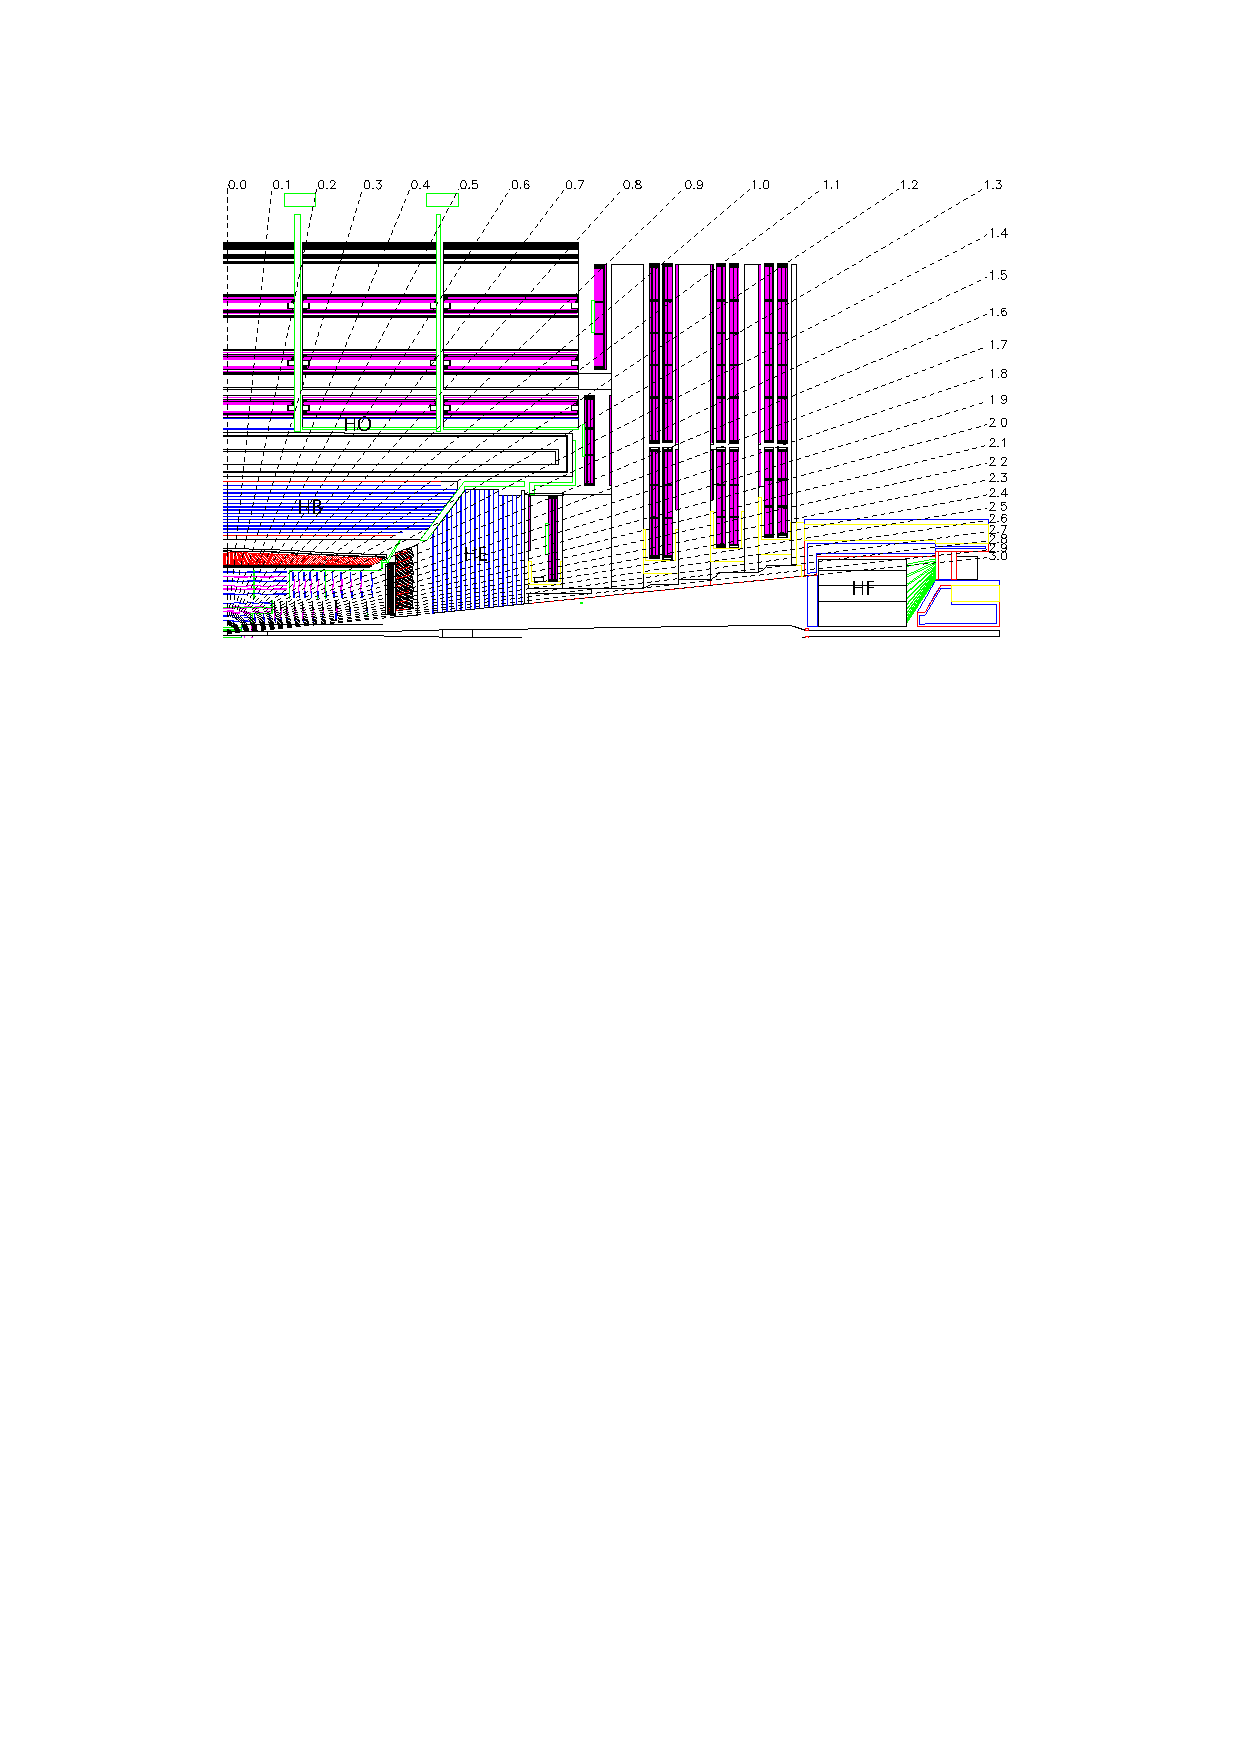
\includegraphics[width=\columnwidth]{HCAL}
    \caption{Longitudinal view of the CMS detector showing the locations of the hadron barrel (HB), endcap (HE), outer
    (HO) and forward (HF) calorimeters \autocite{CMS}.}
    \label{HCAL}
  \end{center}
\end{figure}

As shown in Figure~\ref{HCAL}, HCAL consists of four subsystems: the hadron barrel calorimeter (HB), the hadron endcap
calorimeter (HE), the hadron outer calorimeter (HO) and the hadron forward calorimeter (HF). The barrel and endcap parts
(HB, HE) cover the pseudorapidity range up to \abs\eta \num{<3.0}, and the forward part (HF) extends it to a total
coverage of \abs\eta \num{<5.0}. HCAL surrounds ECAL from its outer limit of \SI{1.77}{\metre} from the beamline, to the
inner limit of the magnet coil at \SI{2.95}{\metre} from the beamline. However, due to space limitations the barrel
calorimeters do not contain complete hadronic showers, therefore an outer calorimeter (HO) was designed to measure the
energy leakage. It is placed in the muon system just outside of the solenoid in the barrel region.

HCAL is a sampling calorimeter consisting of alternating layers of brass and stainless steel absorbers, and plastic
scintillators as active elements. The choice of the absorber material was caused by its short hadronic interaction
length and its property of being non-magnetic, which is crucial in the strong magnetic field of the CMS magnet. The
scintillation light is guided by embedded wavelength-shifting (WLS) fibres. The light from the WLS is then transmitted
via a network of clear fibres, arranged in read-out towers, to hybrid photodiodes (HPDs) \autocite{CMS}.

Both HB and HE scintillators have a granularity of $\Delta \eta \times \Delta \phi =$ \num{0.087x0.087} for \abs\eta
\num{<1.6}, and $\Delta \eta \times \Delta \phi =$ \num{0.17x0.17} for \abs\eta \num{>=1.6}. The tower segmentation of
the forward calorimeter (HF) varies from $\Delta \eta \times \Delta \phi =$ \num{0.175x0.175} at \abs\eta \num{=3.0} to
$\Delta \eta \times \Delta \phi =$ \num{0.3x0.35} at at \abs\eta \num{=5.0}. The HF is placed at about \SI{11}{\metre}
from the interaction point, and is essential to reconstruct very forward hadron jets. Together with HO, it provides the
hermeticity of the calorimetry system, making it possible to measure the transverse missing energy to a reasonable
precision.

\textit{[perhaps need to add the energy resolution plots]}

\subsection{Superconducting Magnet}
The superconducting solenoid is a central feature of the CMS apparatus, essentially giving it its name. The magnet
has a length of \SI{12.5}{\metre}, diameter of \SI{6.3}{\metre} and mass of \SI{220}{\tonne}. Although it was initially
designed to sustain a uniform magnetic field of \SI{4}{\tesla} within the \SI{5.9}{\metre} diameter free bore, operation
at \SI{3.8}{\tesla} was chosen in order to increase the lifetime. The magnetic field is returned by a massive iron yoke.
The main parameters of the CMS magnet are shown in Table~\ref{solenoid_parameters}.

\begin{table}[htbp]
\caption{Parameters of the CMS superconducting solenoid \autocite{CMS_TDR1} \autocite{CMS_Solenoid}.}
\label{solenoid_parameters}
\begin{center}
\begin{tabular}{|l|l|}
  \hline             
  Field & \SI{3.8}{\tesla} \\
  \hline
  Inner Bore & \SI{5.9}{\metre} \\
  \hline
  Length & \SI{12.5}{\metre} \\
  \hline
  Number of Turns & \num{2168} \\
  \hline
  Current & \SI{18160}{\kilo\ampere} \\
  \hline
  Stored energy & \SI{2.3}{\giga\joule} \\
  \hline
\end{tabular}
\end{center}
\end{table}

The large bending power of the solenoid is required to bend the tracks of high energy charged particles to an extent
where good momentum resolution is achieved. The design requirement for the strength of the magnetic field was the
ability to unambiguously determine the sign of the electric charge for muons with a momentum of \SI{\approx 1}{\TeV/c}
\autocite{CMS_TDR1}.

The solenoid coil is constructed from four layers of superconducting high-purity niobium-titanium cable co-extruded with
pure aluminium, which acts as a thermal stabiliser. The cold mass is cooled down to \SI{4.5}{K} by liquid helium. If a
fast discharge happens (e.g.\ caused by a magnet quench), about 3 days are necessary to re-cool the coil.

\subsection{Muon System}
The last sub-detector placed on the outermost part of CMS is the muon system. Since the muons are the most penetrating
particles detectable by CMS, they have the cleanest signature and play an important role in many physics analyses. Due
to their ability to travel through the many layers of the calorimeters, muons are relatively easy to identify and
separate from the background.

\begin{figure}[htbp]
  \begin{center}
    \leavevmode
    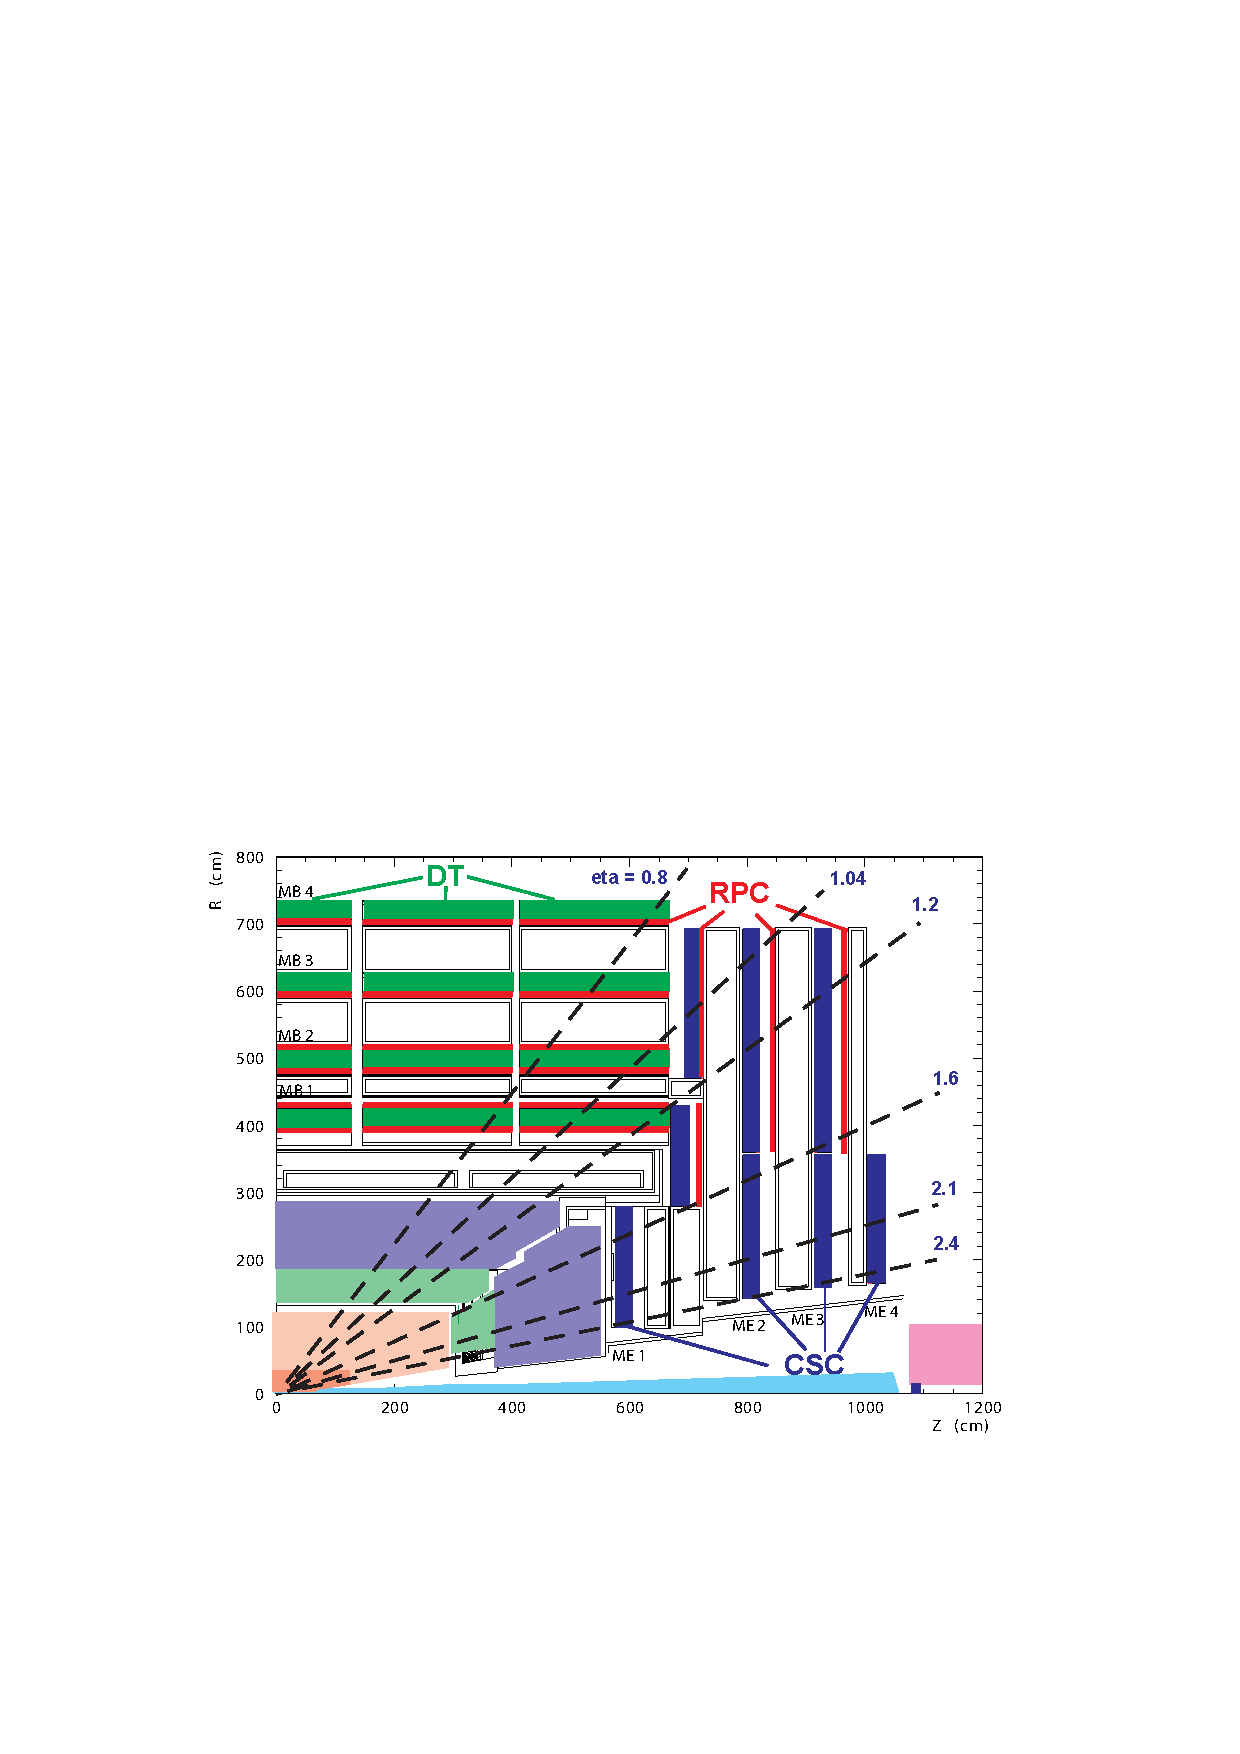
\includegraphics[width=\columnwidth]{muon_system}
    \caption{Layout of one quarter of the CMS muon system. Four drift tube (DT, in light orange) stations are labeled MB
    (“muon barrel”) and the cathode strip chambers (CSC, in green) are labeled ME (“muon endcap”). Resistive plate
    chambers (RPC, in blue) are in both the barrel and the endcaps of CMS, where they are labeled RB and RE,
    respectively.}
    \label{muon_system}
  \end{center}
\end{figure}

The layout of the CMS muon system is shown in Figure~\ref{muon_system}. It consists of the drift tubes (DT), cathode
strip chambers (CSC) and resistive plate chambers (RPC). The entire system surrounds the solenoid and covers the
pseudorapidity region of \abs\eta \num{<2.4}.

The drift tubes are located in the barrel region (\abs\eta \num{<1.2}). Consisting of four stations, they form
concentric cylinders around the beam line; there are \num{250} drift chambers with about \num{172000} sensitive wires in
total. When a muon passes through the volume, it knocks electrons off the atoms of the gas, which then follow the
electric field and reach the positively-charged wires, providing information on the muon's position. The chambers are
filled with the gas mixture of \SI{85}{\percent} $\textrm{Ar}$ and \SI{15}{\percent} $\textrm{CO}_2$, where the muon
drift time does not exceed \SI{380}{\ns}. Although this value is bigger than the typical bunch crossing time (\num{25}
or \SI{50}{\ns}), it is sufficient because of the small muon rate in this region.

In the endcaps, the cathode strip chambers cover the pseudorapidity region of \num{0.9} $<$\abs\eta\num{<2.4}. Each of
\num{468} CSCs is a trapezoidal multi-wire proportional chamber consisting of 6 gas gaps with a plane of radial cathode
strips and a plane of anode wires which are roughly perpendicular. A charged muon traversing each plane of a chamber
causes gas ionisation and a subsequent electron avalanche which produces a charge on the anode wire and an image charge
on the cathode strips. The gas used in CSCs is a mixture of $\textrm{Ar}$, $\textrm{CO}_2$ and $\textrm{CF}_4$.

The resistive plate chambers system is complementary to both DT and CSC systems, and is located in both barrel and
endcap regions (\abs\eta\num{<2.1}). RPCs also operate in avalanche mode with a gas mixture of C$_2$H$_2$F$_4$,
C$_4$H$_{10}$ and $\textrm{SF}_6$, and due to an excellent time resolution of about \SI{1}{\ns} they provide fast
information for triggering. The spacial resolution is, however, quite limited (\SI{\approx 1}{\cm}, compared to
\SI{\approx 100}{\micron} for DTs and CSCs). %http://arxiv.org/abs/1306.6905

\begin{figure}[htbp]
  \begin{center}
    \leavevmode
    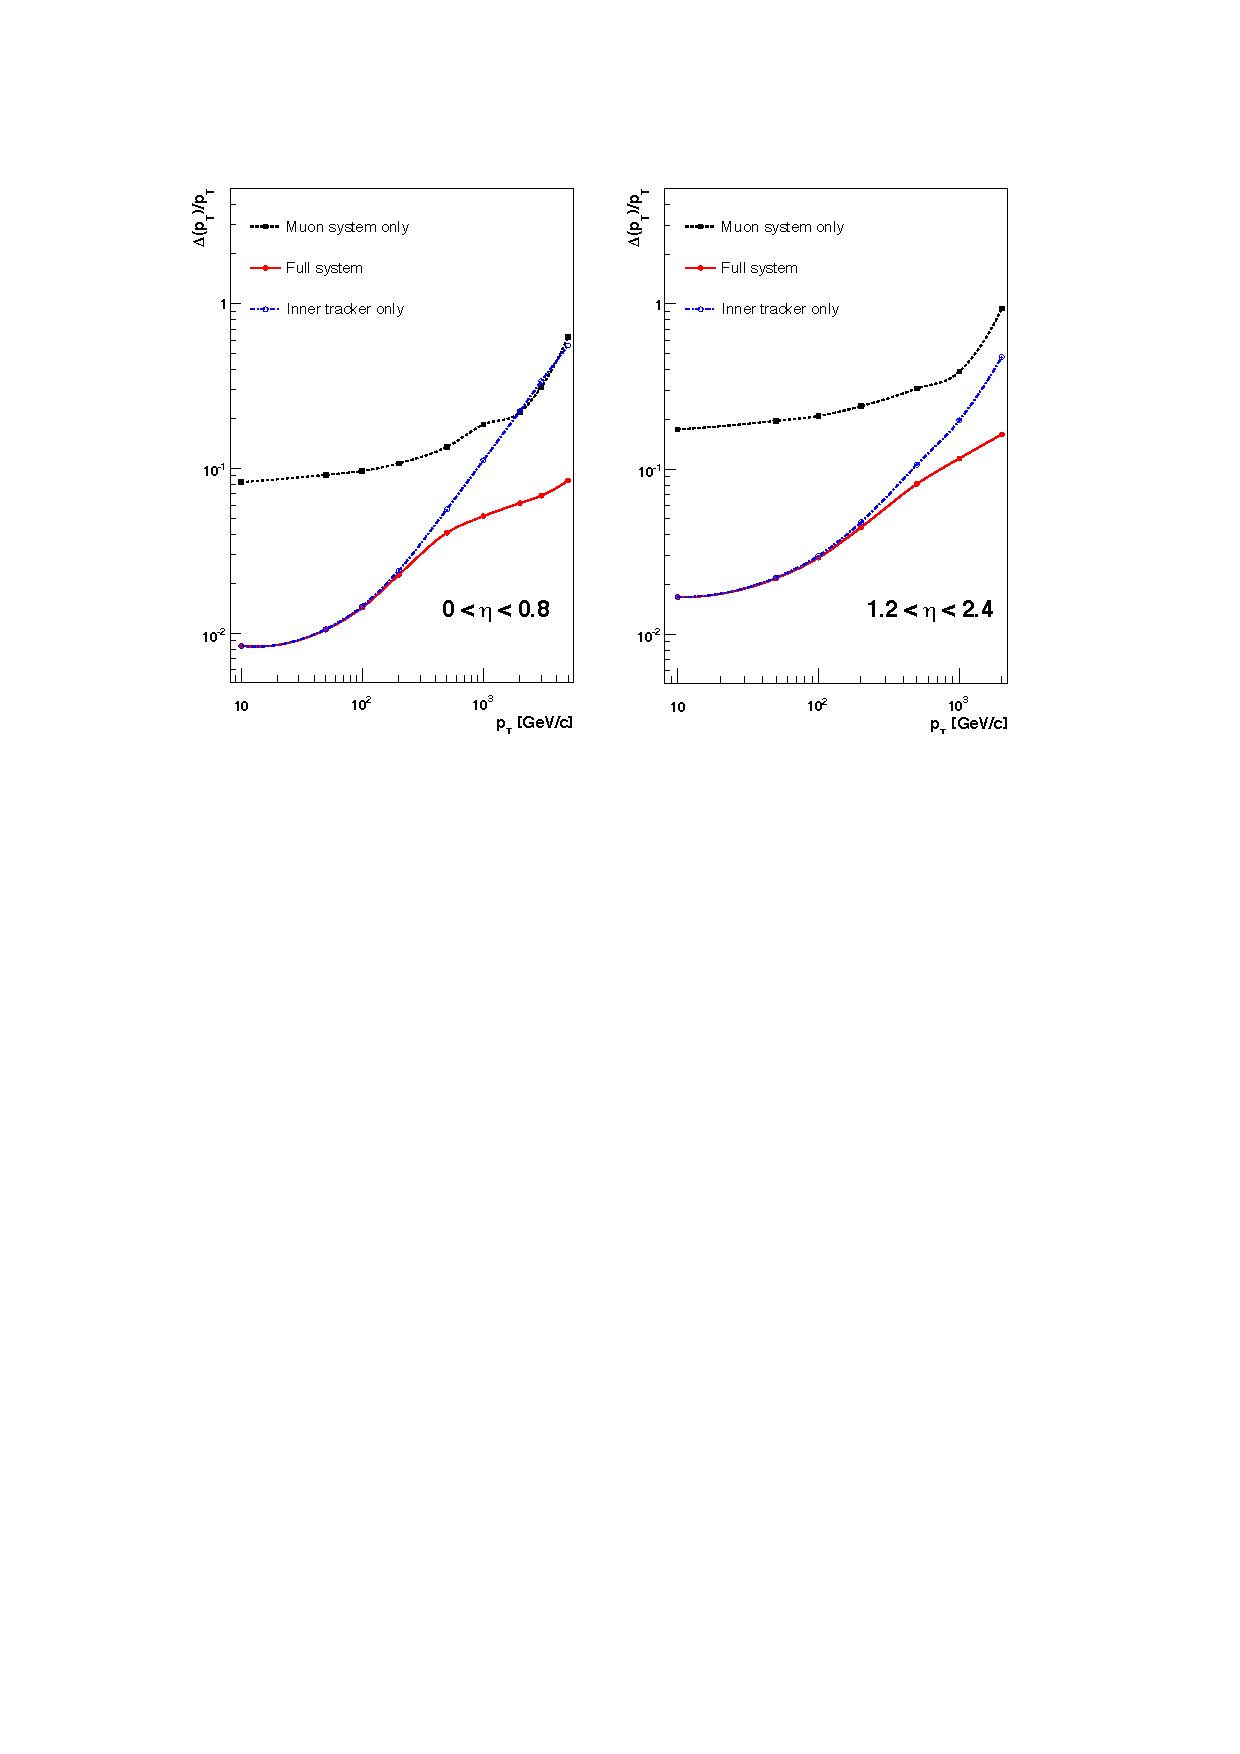
\includegraphics[width=\columnwidth]{muon_resolution}
    \caption{The muon transverse momentum resolution as a function of the transverse momentum (\pt) using the muon
    system only (black), the inner tracking only (blue), and both (red), in regions of \abs\eta \num{<0.8} (left) and
    \num{1.2} $<$\abs\eta\num{<2.4} (right) \autocite{CMS}.}
    \label{muon_resolution}
  \end{center}
\end{figure}

The muon momentum is measured in both the tracker and the muon system.  As it can be seen on
Figure~\ref{muon_resolution}, both sub-systems contribute to the momentum resolution at different \pt values. This
happens due to the difference in the magnetic field and detector technology. For low-\pt muons, the best momentum
resolution is obtained in the tracker, whereas in the high-\pt region the muon system provides a significant
improvement. Therefore, by using information from both the silicon tracker and the muon chambers (i.e.\ reconstructing
the ``global muon''), the momentum resolution is improved in the whole \pt region up to a \SI{\approx 1}{\TeV/c} level.

\subsection{Trigger and Data Acquisition}
\label{ss:trigger_daq}
At design LHC luminosity of $L = $ \SI{d34}{\cm^{-2} s^{-1}}, approximately \num{25} collisions are expected to occur at
each crossing of the proton bunches. The bunch spacing of \SI{25}{\ns} corresponds to a crossing rate of
\SI{40}{\mega\hertz}. Since every event produces \SI{\sim1}{\mega\byte} of raw data, it corresponds to a total data
production of \SI{40}{\tera\byte\per\second}. Attempting to store all of this data is clearly beyond the available
technology. Moreover, only a fraction of events contain hard scattering processes that are of interest, therefore an
effective trigger system had to be implemented.

The CMS trigger is a two-level system, consisting of two independent parts: the Level-1 (L1) trigger and the High-Level
Trigger (HLT). The L1 trigger is a hardware system implemented in programmable electronics residing partly on detector,
and partly in the underground control room located at approximately \SI{90}{\metre} from the experimental cavern. The
maximum latency between the collision and the L1 accept decision received by front-end electronics is
\SI{3.2}{\micro\second}. During this amount of time, the complete event information is buffered in pipelined memories
on the detector. The only information used for the L1 trigger decision is that from the muon system and the calorimetry.
Since the reconstruction of tracks exceeds the time scale required for the L1 decision, the tracker information can't be
used. The L1 trigger reduces the event rate from \SI{\sim40}{\mega\hertz} to \SI{\sim100}{\kilo\hertz}, corresponding to
a data flow of about \SI{100}{\giga\byte\per\second}. These events are fed into the HLT system.

The High-Level Trigger is a software system implemented in a single CPU farm, sometimes referred to as the ``Event
Filter Farm''. Having access to the full event information, customised algorithms of increasing complexity are used
which results in a highly flexible trigger system. The event rate is reduced down to \SI{\sim300}{\Hz}, with the final
data rate of approximately \SI{300}{\mega\byte\per\second} being stored on a large disk cache at the experimental site
(the Storage Manager) and later on transferred to CERN Tier 0 for further processing (see Section \ref{s:computing}).

Since the start of the LHC running, the operating conditions have been changing drastically. During the start-up year of
2010, the instantaneous luminosity went up from about \SI{d27}{\cm^{-2} s^{-1}} to approximately \SI{0.2d32}{\cm^{-2}
s^{-1}}. In 2011 the luminosity ramped up to a factor of \num{20} above that of 2010, reaching approximately
\SI{4d33}{\cm^{-2} s^{-1}}. This required a lot of continuous effort to control the trigger rates at reasonable level,
whilst also keeping its efficiency acceptable. In 2012 the luminosity was more stable, peaking at
\SI{\approx7.6d33}{\cm^{-2} s^{-1}} which is just a factor of 2 above the 2011 values. However, it still came as a
challenge because of the impact of pile-up. At a bunch spacing of \SI{50}{\ns} and increased centre-of-mass energy of
\SI{8}{\TeV}, the average number of pile-up vertices nearly doubled comparing to that in 2011, which required a major
CPU extension and implementation of sophisticated PU mitigation techniques at the HLT level. The author's contribution
to the HLT development of the trigger paths important for top physics is described in Chapter~\ref{c:service_work}.

\section{Computing}
\label{s:computing}
The vast amounts of data delivered by the CMS detector impose high requirements on the offline computing system. During
2010--2012 operation, CMS collected \SI{\sim10}{\peta\byte} of raw data per year. Including Monte Carlo simulations,
reconstructed data and analysis skims, the total annual amount of data essentially doubles. To handle the distributed
storage and processing of this data, not just for CMS but for the entire high energy physics community using the LHC, a
worldwide LHC computing grid (WLCG) has been put in place.

WLCG is a global collaboration of more than 150 computing centres in about 40 countries. The grid has a tiered
architecture, comprising 4 tiers with different resources and services. The first one, Tier 0, is based at CERN and is
responsible for data-taking. It accepts raw data from the data acquisition system and repacks it into primary datasets
according to the trigger information. The raw data is archived to tape, and is also prompt-reconstructed (within 48
hours) before being distributed to the Tier 1 (T1) centres around the world. There are 8 T1 sites based at large
national laboratories in collaborating countries (e.g.\ RAL in the UK and FNAL in the US). Each of the T1 centres is
used for large-scale centrally organised data-processing activities. The data is then distributed in the reduced format
(see Section~\ref{ss:edm}) to a more numerous set of Tier 2 centres, typically located at collaborating universities.
Each of these centres is used for the grid-based analysis and Monte Carlo simulation for the whole experiment, as well
as local services for groups maintaining them. The last stage of computing system, Tier 3, is meant solely for the local
institution's user analysis.

\subsection{Event Data Model}
\label{ss:edm}
In the basis of the CMS Event Data Model lies the concept of an event, which is physically a result of a single
collision in the LHC. From a software point of view, the event is a \Cplusplus object container storing raw data from a
single readout of detector electronics (e.g.\ hits in various sub-detectors), as well as reconstructed data which is
based on this information, such as tracks, clusters and physics objects. All these \Cplusplus objects are stored in ROOT
format \autocite{ROOT}.

The EDM makes use of three main data formats, based on different levels of detail and precision:
\begin{itemize}
  \item RAW format, containing full information from the detector as well as L1 and HLT trigger decisions, with the
  event size of \SI{\sim1.5}{\mega\byte}.
  \item RECO (reconstructed data) format, which is obtained from raw data by application of pattern recognition and
  compression algorithms. This data includes reconstructed detector hits, clusters and physics objects (electrons,
  muons, etc.). The typical event size is \SI{\sim250}{\kilo\byte}.
  \item AOD (Analysis Oriented Data) format, produced by filtering the RECO data from the reconstructed detector
  objects, leaving just the high-level physics objects required for analysis. The event size is reduced down to
  \SI{\sim50}{\kilo\byte}.
\end{itemize}

The RECO and AOD data are analysis-ready data formats, produced centrally and used by many physics analysis groups.
However, further simplification of the data is also a common practice. By transforming the \Cplusplus objects produced
by CMS software into plain basic types or vectors of them, only including the analysis-specific content, the event size
can be reduced down to \SI{\sim3}{\kilo\byte} level depending on the needs of a particular analysis. This data format is
often referred to as private ``ntuples'', and it requires specific analysis software capable of restructuring the data
into user-defined classes. By following this approach, the analysis can be run locally and generally much faster than
processing the RECO or AOD data. However, it requires ``ntuplising'' this data every time when new centrally-recommended
physics objects or corrections are produced.

\subsection{Analysis Software}
\label{ss:analysis_software}
Both of the analyses described in this thesis use the CMS software framework (CMSSW \autocite{CMSSW}), as well as
Bristol Analysis Tools (BAT \autocite{BAT}). The differential cross section analysis also uses an additional level of
python scripts for post-processing \autocite{DailyPythonScripts}.

CMSSW is the key CMS software framework built around the Event Data Model (see Section~\ref{ss:edm}). The framework is
essential for purposes of Monte Carlo simulation, detector calibration and alignment, as well as data reconstruction
and analysis. CMSSW has a modular architecture, consisting of one configurable executable (cmsRun) and a large set of
plug-in modules that contain all the code needed for event processing (reconstruction algorithms, calibration, etc.).
Different versions of CMSSW were used for different analyses: 

\begin{itemize}
  \item \verb!CMSSW_4_2_8! for the top mass analysis on 2011 data;
  \item \verb!CMSSW_4_4_4! for the missing transverse energy analysis on 2011 data;
  \item \verb!CMSSW_5_3_9! for the top cross pair cross section analysis on 2012 data.
\end{itemize}

Corresponding versions were used to produce ntuples for processing by BAT, which was used to read the data, apply
selections, calculate high-level variables and to create various histograms of distributions. BAT was originally started
in 2010 by Dr.\ Lukasz Kreczko for the needs of the Bristol top group, later on also developed by the author and other
researchers from Bristol and affiliated top groups. Like CMSSW, this framework has a modular structure, with its classes
falling in four main categories:

\begin{itemize}
  \item readers, for translating plain data types from ROOT files into \Cplusplus objects;
  \item RECO objects, i.e.\ output of the readers (physical objects like leptons, jets and its collections);
  \item selections, for application of event selections;
  \item analysers for creating histograms, applying selections, algorithms, and filling histograms.
\end{itemize}

All analysers are independent from each other, making the analysis chain stable and reliable. The final set of python
scripts is used to prepare the histograms, perform fitting and unfolding procedures (in case of cross section analysis),
and producing final tables and plots. Rootpy package \autocite{rootpy} was used to access ROOT libraries in python
interface, and matplotlib \autocite{matplotlib} was used to create plots.

\section{Object Reconstruction}
\label{s:object_reconstruction}
Most CMS analyses, including the ones described in this thesis, adopt a reconstruction technique called Particle Flow
(PF) \autocite{PF}. This algorithm is used to obtain a global event description at level of individually reconstructed
particles by means of combining information coming from all sub-detector systems. The ultimate goal is to determine
type, energy and momentum of all the particles in the event with highest possible precision and in the most optimal way.
The types of these particles include electrons, muons, charged hadrons, neutral hadrons and photons. All these particles
are then used to reconstruct jets (Section~\ref{ss:jet_reconstruction}), missing transverse energy
(Section~\ref{ss:electron_reconstruction}) and tau leptons from their decay products.

\subsection{Electron Reconstruction}
\label{ss:electron_reconstruction}
The reconstruction of the \ttbar pair with an electron in the final state imposes high requirements on the electron
identification and its energy-momentum measurement, precision of which is of major importance for both top mass and
\ttbar cross section measurements.

Although the CMS detector is equipped with highly accurate ECAL and tracker systems, electron identification and
reconstruction is still a challenging task due to the large amount of tracker material (see Section~\ref{ss:tracker}).
This results in a significant Bremsstrahlung photon emission, which often causes an ECAL energy deposit to be widely
spread in azimuthal direction because of the high magnetic field. Therefore, dedicated algorithms were developed in
order to collect all Bremsstrahlung energy deposits in the calorimeter (Bremsstrahlung recovery), and also to take into
account the kinks in the electron trajectory caused by photon emissions.

Electron reconstruction in CMS has following distinct stages: seeding, track finding, pre-identification, Bremsstrahlung
recovery, track-cluster linking and final identification. Historically, the original seeding algorithm was designed and
optimised for isolated high-\pt electrons. This approach starts from ECAL clusters, and therefore is called the
'ECAL-driven' seeding. It is based on the property of the ECAL energy deposits to have narrow width in the $\eta$
coordinate, and to be widely spread in $\phi$ (azimuthal direction) like it was mentioned above. The electron and all
the associated Bremsstrahlung energy deposits form a single ``super-cluster'', and the ability to correctly determine it
affects the overall performance of this method. Only super-clusters with transverse energy above \SI{4}{\GeV} are taken
into account. Super-clusters are then matched to pairs or triplets of hits in the inner tracker layers, forming the
track seeds on which the electron tracks are built upon.

The performance of the ECAL-driven method is not very well suited for non-isolated and low-\pt electrons. This occurs
mainly due to the fact that the super-cluster position and energy can be highly biased by the impact of overlapping
particles, especially if the electron happens to be within a jet and therefore non-isolated. Also, high track
multiplicity complicates the backward propagation from a super-cluster, because it can be consistent with a number of
track seeds corresponding to other particles. To minimise the number of these fake seeds, the ratio between the HCAL and
ECAL energy deposits ($H/E$) is required to be smaller than \num{0.15}. The HCAL towers used in the calculation of this
ratio are taken within a cone of $\DR = 0.3$ behind the super-cluster position. Although this helps to keep the fake
seed rate under control, the efficiency for non-isolated electrons becomes rather limited. As for the low-\pt electrons,
the wider azimuthal spread of Bremsstrahlung photons leads to poorer reconstruction of the super-cluster, biasing its
position and therefore preventing the efficient matching with a track seed.

Within the particle flow method, efficient reconstruction of non-isolated and low-\pt electrons is particularly
important since it affects the reconstruction of jets and missing transverse energy. Therefore, a different
('tracker-driven') seeding algorithm is used, which starts from reconstruction of tracks. The baseline of the CMS track
reconstruction is the Kalman filter (KF) \autocite{KF}, which is a linear least-squares estimator based solely on
Gaussian probability density functions. It is particularly suitable for muon reconstruction since it is dominated by
multiple Coulomb scattering and its impact is well modelled by Gaussian fluctuations. However, this approach usually
fails for electrons because Bremsstrahlung photon emission is highly non-Gaussian. To accommodate for the resulting
kinks in the electron trajectory, the Gaussian-Sum Filter (GSF) \autocite{GSF} is used, which is essentially a
non-linear generalisation of the Kalman Filter. In this method, Bremsstrahlung energy loss is modelled by a Gaussian
mixture, therefore GSF track fit provides a better estimate for the inner and outer track momentum comparing to the KF
algorithm. The downside of this approach is its high CPU usage, which means it can be run on a limited number of seeds.

The GSF tracks are reconstructed upon all ECAL-driven seeds. In case of the 'tracker-driven' seeds, a pre-identification
based on high-purity KF tracks has been adopted. This procedure starts with the tracks reconstructed with very tight
criteria, thus decreasing the fake rate yet compromising on tracking efficiency. Then an iterative-tracking strategy is
carried out by means of removing hits unambiguously assigned to tracks from the previous iteration, and also
progressively relaxing track seeding criteria. This approach leads to both high efficiency and low fake rate, which is
crucial for low-\pt and non-isolated electrons.

In the next step, track-cluster matching has to be performed. In case if electron has negligible Bremsstrahlung
emission, the track is well reconstructed with the KF algorithm all the way to the ECAL internal surface, where the
closest cluster is matched to the track. The corresponding cluster energy is compared with the track momentum, and if
the ratio ($E/p$) is close to unity, the track is selected. On the contrary, if the electron experiences a significant
Bremsstrahlung emission, other track characteristics have to be exploited. In this case a selection based on the number
of hits in the tracker and the $\chi^2_\textrm{KF}$ of the KF fit is applied before running a GSF refit. Finally, the
number of hits, the GSF refit $\chi^2_\textrm{GSF}$, $\chi^2_\textrm{KF}/\chi^2_\textrm{GSF}$ ratio, the energy loss
measured by the track and the quality of the ECAL cluster-track matching are fed into a multivariate analysis using a
Boosted Decision Trees (BDT) estimator.

Both tracker-driven and ECAL-driven seeds are used to obtain the GSF track collection of electron candidates. In the
particle flow algorithm, it is necessary to link both electron and Bremsstrahlung energy deposits to the GSF track. A
super-cluster is linked to a track if the extrapolated position from the outermost tracker measurement is within the
boundaries of one of the ECAL cells at the expected depth of the electron shower maximum. The preshower-ECAL and
ECAL-HCAL links are made in a similar way.

Another important particle flow procedure, also driven by GSF tracks, is Bremsstrahlung recovery. In order to
reconstruct an electron with correctly assigned energy and momentum, it is crucial to identify all energy deposits from
Bremsstrahlung photons, thus forming a super-cluster. This procedure is carried out for each tracker layer by computing
a straight-line extrapolation tangent to the track, up to the calorimeter. To determine a Bremsstrahlung photon,
track-cluster linking is performed as described above. To limit the charged hadron contamination, clusters already
assigned to KF tracks are not included in the calculation. Also, the distance in $\eta$ coordinate between the
extrapolation and the cluster is required to be smaller than \num{0.015}, which helps to reduce the neutral particles
background.

\subsubsection{Electron Identification}
\label{sss:electron_id}

Electron reconstruction in CMS is based on a characteristic signature that electrons leave in the tracker and
calorimetry systems. However, other objects like charged hadrons, jets or photon conversions can produce very similar
signatures and therefore may be reconstructed as electrons. Therefore, in order to distinguish these ``fake'' electrons
from ``real'' ones, a further selection has to be applied. This procedure is referred to as electron identification (or
electron ID).

Initially the electron identification is performed at the final stage of the electron reconstruction process. The
working points of the cuts applied are selected to be loose enough in order to satisfy most CMS analyses requirements.
Afterwards, more specific (tighter) ID cuts are applied for each individual analysis, defining the working point in the
trade-off between selection efficiency and fakes contamination. This will be discussed separately in the selection
description for each analysis in corresponding chapters.

There are several electron identification algorithms used by various CMS analyses, and four of them are used in the
analyses described in this thesis: simple cut-based (SCB ID), cuts in categories (CiC ID), particle flow (PF ID) and
multi-variate analysis (MVA ID).

Simple cut-based identification is used in the High-Level Trigger, and therefore has to be as simple, fast and
robust as possible. Cuts are applied on the following variables:

\begin{itemize}
  \item $H/E$, i.e.\ the ratio of hadronic energy of the HCAL towers centred at the super-cluster position of the
  electron in a cone of radius $\Delta R = 0.15$, and the super-cluster electromagnetic energy;
  \item $\Delta\eta_{\text{in}}$, i.e.\ the difference in $\eta$ between the extrapolated track position and $\eta$ of
  the super-cluster;
  \item $\Delta\phi_{\text{in}}$, i.e.\ the difference in $\phi$ between the extrapolated track position and $\phi$ of
  the super-cluster;
  \item $\sigma_{i\eta, i\eta}$, i.e.\ cluster shape of the electron energy in a $5\times5$ block of crystals around the
  seed crystal (the one with the highest energy) \autocite{electron_reconstruction}:
  \begin{equation}
  \label{eq:cluster_shape}
    \sigma_{i\eta, i\eta} = \sum_{5\times5 \text{ crystals}} \left(\eta_i - \eta_\text{seed cluster}\right)^2
    \frac{E_i}{E_{\text{seed cluster}}}
  \end{equation}
\end{itemize}

Although this identification method has an advantage of its simplicity, it does not show the best signal efficiency and
background rejection. One of the more complex methods is the CiC ID, which exploits the categorisation of electrons. It
is optimised to select electrons from different sources (W, Z and J/$\psi$ decays) and reject fakes from jets or
conversions. In order to achieve higher efficiency, electron candidates are split into categories with different signal
to background ratio, allowing to better tune the working points of the cuts. The first step in categorisation is done by
division between barrel and endcap regions of the detector. Since the properties of both the tracker and calorimetry
systems differ significantly in these two regions, different cuts are applied. The second step is based on the following
observables:

\begin{itemize}
  \item $f_\text{brem}$, or measured bremsstrahlung fraction, defined as:
  \begin{equation}
  \label{eq:fbrem}
    f_\text{brem} = \frac{p_\text{in}-p_\text{out}}{p_\text{in}}
  \end{equation}
  where $p_\text{in}$ is the initial track momentum at the vertex and $p_\text{out}$ is the track momentum at the last
  hit;
  \item $E/p$, which is the ratio of the super-cluster energy and the initial track momentum.
\end{itemize}

Three categories of electron candidates are distinguished \autocite{CiC_ID}:
\begin{itemize}
  \item ``Low-Brem'': $0.9 < E/p < 1.2 - f_\text{brem} < 0.12$ (barrel), $0.82 < E/p < 1.22 - f_\text{brem} < 0.2$
  (endcap), the fake-like region with high number of both real and fake electrons;
  \item ``Bremming'': $0.9 < E/p < 1.2 - f_\text{brem} > 0.12$ (barrel), $0.82 < E/p < 1.22 - f_\text{brem} > 0.2$
  (endcap), the electrons-like region with a little contamination from fakes;
  \item ``Bad-Track'': remaining regions with a low number of real electrons.
\end{itemize}

The third and the final step in categorisation is based simply on the electron transverse energy, with the lower
threshold taken as \SI{10}{\GeV}. In each category, the selection is performed on the basic ID variables already
mentioned above for the simple cut-based identification. On top of these variables, isolation and conversion rejection
variables are also used, they are discussed in Section~\ref{sss:electron_isolation} and
Section~\ref{sss:photon_conversions}, respectively.

The cuts within CiC ID are applied in order to maximise the signal to background ratio. Depending on the needs of
different analyses, nine levels of cut severity are implemented: \textit{VeryLoose, Loose, Medium, Tight, SuperTight,
HyperTight(1-4)}. Each step decreases the fake rate by about a factor of two for electrons with \ET$>$ \SI{20}{\GeV}
\autocite{CiC_ID}. The CiC ID is used as a primary electron identification method in the Top Mass analysis
(Chapter~\ref{c:top_mass_analysis}).

Particle flow ID is the final step of the particle flow electron reconstruction. Following the particle flow concept,
is uses information from all the CMS sub-detectors obtained in previous reconstruction steps to build new observables
for electron identification. The complete list of PF ID observables is given below:
\begin{itemize}
  \item \pt and $\eta$ of the GSF track;
  \item GSF $\sigma_{p_\text{T}}/p_\text{T}$, transverse momentum resolution of the GSF track;
  \item \#hits$_\text{KF}$, number of reconstructed KF track hits;
  \item $\chi^2_\textrm{GSF}$ and $\chi^2_\textrm{KF}$, GSF and KF goodness-of-fits;
  \item $\Delta\eta$: distance in $\eta$ between the position of the cluster and the extrapolated position of the
  GSF track;
  \item $\sigma_{\eta\eta}$, cluster shape (Equation~\ref{eq:cluster_shape}) of the ECAL cluster linked to the
  GSF track;
  \item $H/(H+E_\text{e})$, hadron fraction of the shower, where $H$ is the energy of the hadron cluster linked to
  the GSF track;
  \item $(E_\text{e}+\sum E_\gamma)/p_\text{in}$, ratio between the super-cluster energy and the inner track
  momentum;
  \item $E_\text{e}/p_\text{out}$, ratio between the electron cluster energy and the track outer-momentum;
  \item $\sum E_\gamma/(p_\text{in}-p_\text{out})$, the ratio between the Bremsstrahlung photon energy as measured by
  ECAL and by the tracker;
  \item $EarlyBrem$, flag of $(E_\text{e}+\sum E_\gamma)>p_\text{in}$ inequality, corresponding to an electron
  emitting an ``early'' Bremsstrahlung photon, i.e.\ before it has crossed at least three tracker layers;
  \item $LateBrem$, flag of $E_\text{e}>p_\text{out}$ inequality, corresponding to an electron emitting a ``late''
  Bremsstrahlung electron, when the ECAL clustering is not able to disentangle the overlapping electron and photon
  showers;
  \item $f_\text{brem} = (p_\text{in}-p_\text{out})/p_\text{in}$, Bremsstrahlung fraction (Equation~\ref{eq:fbrem}).
\end{itemize}

All these variables are combined into a single discriminator by a multivariate analysis technique (BDT method), which
has been trained on signal and background Monte Carlo samples. PF ID is a relatively loose identification method, since
it has to satisfy the needs of all analyses using particle flow collections.

Finally, MVA electron identification is used in top cross sections analysis on 2012 data. It is another multivariate
analysis technique, optimised to select isolated electrons from W and Z decays. The variables used in MVA ID are also
combined into a single discriminator, they are largely similar to the ones used in PF ID:

\begin{itemize}
  \item \pt and $\eta$ of the GSF track;
  \item \#hits$_\text{KF}$, number of reconstructed KF track hits;
  \item $\chi^2_\textrm{GSF}$ and $\chi^2_\textrm{KF}$, GSF and KF goodness-of-fits;
  \item $\Delta\eta$: distance in $\eta$ between the position of the cluster and the extrapolated position of the
  GSF track;
  \item $\Delta\phi$: distance in $\phi$ between the position of the cluster and the extrapolated position of the
  track;
  \item $\Delta\eta_{vtx}$: distance in $\eta$ between the position of the cluster and the position of the GSF track
  at vertex;
  \item $\Delta\phi_{vtx}$: distance in $\phi$ between the position of the cluster and the position of the GSF track
  at vertex;
  \item $\sigma_{\eta \eta}$, cluster shape in $\eta$;
  \item $\sigma_{\phi \phi}$, cluster shape in $\phi$;
  \item $\eta$ width of the super-cluster;
  \item $\phi$ width of the super-cluster;
  \item $H/E$, ratio of HCAL and ECAL cluster energy;
  \item $E_\text{super-cluster}/p_\text{T}$, ratio between the super-cluster energy and the track momentum;
  \item $1/E_\text{super-cluster} - 1/p_\text{T}$, difference between inverse super-cluster energy and inverse
  track momentum;
  \item $E_\text{e}/p_\text{out}$, ratio between the electron cluster energy and the track outer-momentum;
  \item $1-E_{1\times 5}/E_{5\times 5}$, where $E_{1\times 5}$ is the energy in the central $1\times 5$ strip of the
  $5\times 5$ electron cluster and $E_{5\times 5}$ its total energy;
  \item $E_{3\times 3}/E_\text{super-cluster, raw}$, ratio of the energy of a cluster of $3\times 3$ and the
  uncorrected (raw) energy of the super-cluster;
  \item $E_\text{PS}/E_\text{super-cluster, raw}$, ratio of the energy in the preshower detector and the raw
  super-cluster energy (only in the endcap region).
  % Surely there are isolation variables? There's no MVA documentation whatsoever. Absolute joke.
\end{itemize}

\subsubsection{Electron Isolation}
\label{sss:electron_isolation}

Isolation is an observable that allows to distinguish prompt electrons (i.e.\ the ones from W and Z decays) from jets
faking electrons and electrons within jets. It is essentially a measure of activity around the particle. In CMS, there
are two different ways of quantifying isolation: detector-based and particle-based. The detector-based isolation is
defined separately for each detector sub-system (tracker, ECAL and HCAL):

\begin{itemize}
  \item Tracker isolation, calculated as the sum of transverse momenta of all track within a cone of $\Delta R = 0.3$
  around the electron, excluding the electron momentum itself;
  \item ECAL isolation, i.e.\ the sum of transverse energy of all ECAL clusters within a cone of $\Delta R = 0.3$
  around the super-cluster position. The footprint of the original electron is also removed;
  \item HCAL isolation, defined as the sum of transverse energy of all HCAL towers within a cone of $\Delta R = 0.3$
  centred at the super-cluster position.
\end{itemize}

Particle-based isolation exploits the particle flow information: it is calculated as the sum of transverse energy of all
PF particles in the cone of $\Delta R = 0.3$ around the electron. Both detector-based and particle-based isolation
definitions are often normalised to the electron transverse momentum (or energy in case of calorimeter isolation) in
order to improve signal efficiency. The normalised sum of the tracker, ECAL and HCAL isolation variables is referred to
as detector-based relative isolation (or \reliso), similarly normalised particle-based isolation is called PF \reliso.
These quantities are crucial in various methods to estimate the QCD background contribution for many analyses, and will
be used for both electrons and muons throughout this thesis.

\subsubsection{Identification of photon conversions}
\label{sss:photon_conversions}
Interacting with detector material, photons can convert into electron-positron pairs. Due to the large amount of
material budget in the tracker (Figure~\ref{tracker_material_budget}), especially in the endcap region, there is a high
chance of conversions to happen. The resulting electrons can successfully fake prompt signal electrons, passing all the
identification criteria and appearing isolated if the initial photon was isolated, too. Therefore conversions constitute
a large proportion of the QCD background to top signal. The electron-positron pair may not be symmetrical in transverse
momenta, therefore a veto on a second electron is not sufficient to reject such electrons and other conversion
identification criteria are necessary.

The simplest method is based on counting the number of missing hits in the tracker. Conversions are most likely to
happen at some distance from the interaction point, essentially anywhere between the point of photon production and the
end of the tracker. Therefore electrons produced in such conversions are likely not to traverse through all the pixel
layers. To separate these electrons from the prompt ones, a cut on the number of missing layers can be used. However,
this approach fails if conversion occurs in the beam pipe, or if the reconstructed electron track is paired with
unrelated hits in the tracker, making it look like a prompt electron.

A slightly more sophisticated method is a partner track method. It is based on geometrical cuts on $dist$ and $dcot$
variables, which refer to the distances between tangent points of any two tracks in the $r-\phi$-plane and $r-z$-plane,
respectively:
\begin{equation}
  dist = \left|\left|\vec{r}_1 - \vec{r}_2 \right|- r_1 - r_2\right|
\end{equation}
\begin{equation}
  dcot = \left|\frac{1}{\tan\theta_1} -\frac{1}{\tan\theta_2}\right|
\end{equation}
Here $\vec{r}_{1,2}$ are radial vectors of the two tracks, $r_{1,2}$ are the track radii and $\theta_{1,2}$ -- angles
between the tracks and the beam pipe. Apart from the cuts on $dist$ and $dcot$ variables, tracks should have opposite
charge in order to be considered to come from a photon conversion.

These two methods for conversion identification were used in the top mass analysis on 2011 data. For the top cross
sections analysis on 2012 data, along with the number of hits method, a more advanced technique called vertex fit was
used. It is essentially a full vertex fit of all pairs of tracks, with the selection being made on the the fit
probability. The method benefits from the full use of track uncertainties and covariances, combining all information
into a single discriminator. However, increased complexity of this technique makes it more CPU-intensive than the
partner track method.

% internal source: https://twiki.cern.ch/twiki/bin/view/CMS/ConversionTools

\subsection{Muon Reconstruction}
\label{ss:muon_reconstruction}
A good muon reconstruction and identification was one of the main CMS design requirements. Initially, muons are
reconstructed independently in the tracker (``tracker tracks'') and in the muon system (``standalone muon tracks'')
using the Kalman Filter technique \autocite{KF}. Based on these objects, two different reconstruction methods are used:
\autocite{muon_reconstruction}

\begin{itemize}
  \item Global muon reconstruction. Each standalone muon track reconstructed in the muon system is matched with the
  tracker track by propagating onto a common surface. A global fit is performed on the combined collection of hits from
  both tracks, and the resulting muon is referred to as a \textit{global muon}.
  \item Tracker muon reconstruction. All tracker tracks above certain threshold (\pt $>$ \SI{0.5}{\GeV}, $p >$
  \SI{0.5}{\GeV}) are extrapolated to the muon system, taking into account possible energy losses, magnetic field and
  multiple Coulomb scattering. If the track matches at least one muon segment in the muon system, i.e.\ a short track
  stub made of DT or CSC hits, it is considered a \textit{tracker muon}.
\end{itemize}

Global muon reconstruction has a high efficiency for high-\pt muons, penetrating through more than one muon station. On
the contrary, tracker muon reconstruction is more efficient for low-\pt muons (\pt $<$ \SI{5}{\GeV}), as it requires
just a single muon segment. Since the \ttbar analyses described in this thesis have a semileptonic signature with
exactly one energetic muon in the final state (in case of the muon channel), only the global muon reconstruction method
is used, as its momentum resolution at high transverse momenta benefits from both the tracker and the muon system
(Figure~\ref{muon_resolution}).

Following the reconstruction, the quality of the muon objects is verified by applying identification criteria. This is
done in order to suppress hadronic punch-through, muons from decays in flight and cosmic muons. Selection is applied on
the following observables:
\begin{itemize}
  \item normalised $\chi^2$ ($\chi^2$/number of degrees of freedom) of the global muon fit;
  \item number of muon chamber hits in the global muon fit;
  \item number of muon stations with muon segments;
  \item transverse impact parameter $d_{xy}$ (closest approach of the track to the primary vertex);
  \item longitudinal distance $d_z$ of the tracker track w.r.t. the primary vertex;
  \item number of hits in the pixel detector;
  \item number of hits in the tracker layers.
\end{itemize}

The muon identification also exploits the CMS particle flow event reconstruction, making use of information coming from
all sub-detectors. Particle flow muons (PF muons) are identified by imposing selection on all muon candidates
reconstructed with the global muon method. This selection was optimised for identification of muons in jets, minimising
the fake rate from misidentified charged hadrons, which is crucial for correct reconstruction of jets and missing
transverse energy (described in more detail in the following sections). Depending on the analysis specifics, isolation
requirements can also be applied; isolation definitions closely follow the ones for electrons
(Section~\ref{sss:electron_isolation}).

%internal source https://twiki.cern.ch/twiki/bin/view/CMSPublic/SWGuideMuonId

\subsection{Jet Reconstruction}
\label{ss:jet_reconstruction}
Hadronisation of quarks and gluons leads to production of narrow cones of particles moving in approximately one
direction, called jets. This happens due to colour confinement, as particles carrying a colour charge cannot exist in
free form, they have to fragment into hadrons before they can be detected directly. Therefore, to measure the initial
parton's momentum and energy, all these particles must be combined into jets.

The CMS particle flow algorithm implies reconstruction of individual particles (charged and neutral hadrons, electrons,
muons, photons) before combining (or clustering) them into jets. A few different jet clustering techniques exist, but
the one used predominantly in CMS and exclusively in this work is \antikt algorithm \autocite{anti-kt}, which defines
the distance between constituent particles as:
\begin{equation}
d_{ij} = \min\left(\frac{1}{k^2_{t,i}},\frac{1}{k^2_{t,j}}\right) \frac{\Delta_{i,j}^2}{R^2}
\end{equation}
where $\Delta_{i,j}^2 = (y_i-y_j)^2 + (\phi_i-\phi_j)^2$, $k_{t,i/j}$, $y_{i/j}$ and $\phi_{i/j}$ are respectively
transverse momenta, rapidities and azimuth angles of particles $i/j$, and $R$ is the radius parameter.

The clustering proceeds by identifying the smallest distances between particles and recombining them until all jets are
formed and no particles are left. An event typically has a few well-separated hard (high-\pt) particles and a large
amount of soft (low-\pt) particles. The distance $d_{1i}$ between a hard particle 1 and a soft particle $i$ will be
fully determined by the transverse momentum of the hard particle and the $\Delta_{1i}$ separation. On the other hand,
distance between soft particles with similar separation will be substantially larger. Therefore, soft particles tend to
cluster around the hard ones before they cluster amongst themselves. On the output, the \antikt algorithm forms
conical jets with boundaries resilient to soft radiation.

\subsubsection{Jet Energy Corrections}
\label{sss:JEC}

Due to non-linear and non-uniform response of the calorimetry systems, jets reconstructed using detector inputs
typically have energies different to the ones of corresponding Monte Carlo particle jets (or generator jets),
reconstructed by clustering the four-momenta of all stable particles generated in Monte Carlo simulation. Therefore some
mapping procedure is necessary. Corrections applied to  reconstructed jets in order to translate the measured energy to
the true particle (or parton) energy are referred to as jet energy corrections, or JEC.

CMS has adopted a factorised approach of applying jet energy corrections, meaning that each correction level takes care
of a different effect. The set of corrections is applied sequentially, i.e.\ the output of each step is the input to the
next one. Essentially, each level of correction is a scaling of a jet four-momentum, with a scale factor depending on
various parameters of the jet, typically pseudorapidity and transverse momentum. Currently, the correction levels go as
follows:

\begin{itemize}
  \item L1 Offset correction;
  \item L2 Relative ($\eta$) correction;
  \item L3 Absolute (\pt) correction;
  \item L4 EMF (electromagnetic energy fraction) correction;
  \item L5 Flavour correction;
  \item L6 UE (underlying event) correction;
  \item L7 Parton correction.
\end{itemize}

The goal of the L1 correction is subtraction of pile-up and electronic noise contributions from the jet energy. The
energy from pile-up vertices can be deposited in calorimeters since the additional proton-proton collisions occur close
enough in time to the hard scattering process. Electronic noise in calorimeter readouts also creates additional energy
offset which needs to be corrected for. The scale factors for L1 correction are derived using data-driven methods
(zero-bias collisions).

The relative L2 correction is designed to flatten the jet response in pseudorapidity. These corrections are extracted
with respect to the barrel region in bins of \pt, and therefore are uncorrelated with the following L3 corrections. Both
Monte Carlo and data-driven (dijet balance) methods are used to derive the L2 scale factors. Once a jet is corrected for
$\eta$ dependence, it is corrected back to the particle level by applying absolute L3 correction. The goal of this
correction is to flatten the jet response in transverse momentum. Derivation of L3 scale factors is done by using Monte
Carlo truth information, or data-driven $Z/\gamma$+jet balance techniques.

The L4 EMF correction takes care of variations in jet response with respect to electromagnetic energy fraction, i.e.\
the fraction of energy deposited in ECAL by hadrons. Although it has been shown that EMF-dependent correction in three
parameters (\pt, $\eta$, EMF) can improve the observed jet resolution, this correction is optional for most CMS analyses
and hasn't been used in this work.

Another optional correction is the L5 flavour correction, which is intended to correct the jets depending on the flavour
of initiating partons, i.e.\ light quarks, heavy ($b$ and $c$ quarks), or gluons. Jets originating from heavy quarks are
different from light quark jets in a few aspects. The average number of charged hadrons within $b$-jets is higher than
the one for the light jets, although the average momentum of charge hadrons is smaller. Moreover, $b$-hadrons have a
larger branching fraction into semileptonic decays with neutrinos in the final state that cannot be detected. All these
factors may lead to a substantially smaller charged hadron energy fraction comparing to the light jets, therefore the
average calorimeter energy response is lower for the $b$-jets. These effects are meant to be taken care of by the L5
correction, which is derived either from Monte Carlo or data-driven \ttbar events.

Underlying event \autocite{underlying_event} refers to all the activity in the proton-proton collision apart from the
process of interest, i.e.\ the hard scattering process. It includes particles coming from additional parton interactions
(or multiple scatterings) and beam remnants. Depending on the analysis goals, underlying event may also include initial
and final state radiation (ISR and FSR) which represent the soft gluon radiation before and after the hard scattering
process, respectively. Underlying event activity results in production of additional soft jets which can bias the jet
energy measurement. Optional L6 UE correction attempts to mitigate such bias. However, it was not used in the analyses
described in this thesis, since underlying event is an intrinsic part of proton-proton interactions effectively modelled
by Monte Carlo simulation. In particular, the top cross sections analysis is designed to be very sensitive to such
higher-order processes, and not taking them into account may result in compromising the discriminating power between
Monte Carlo generators.

Finally, L7 parton correction attempts to correct the jet energies back to the parton level. It is also optional and was
only used in the top mass analysis. The correction factors were derived from Monte Carlo simulations by comparing the
generator jets momenta to their matched partons.

Due to the fact that CMS simulation is not perfectly tuned to the data yet, additional residual L2L3 corrections are
applied in order to achieve better agreement between data and simulation. It is essentially a small residual $\eta$- and
\pt-dependent calibration applied exclusively to data, which will remain in place until CMS develops a perfectly tuned
simulation reproducing the data features out of the box.

%internal source: https://twiki.cern.ch/twiki/bin/view/CMS/IntroToJEC

%Jet energy resolution? https://twiki.cern.ch/twiki/bin/view/CMS/JetResolution

\subsubsection{Particle Flow Jet Identification}
\label{sss:PFJet_ID}
To ensure the quality of the jets, a final identification criteria are applied to all jet objects. Particle flow jet
identification (or PF jet ID) is used to reduce the noise and rate of electrons reconstructed as jets. The cuts are
applied on the following observables :

\begin{itemize}
  \item number of constituent particles;
  \item NHF (neutral hadron energy fraction);
  \item CHF (charged hadron energy fraction);
  \item NEF (neutral electromagnetic energy fraction);
  \item CEF (charged electromagnetic energy fraction).
\end{itemize}

A rather loose identification cuts (referred to as ``loose PF jet ID'') were used in this work: a requirement of more
than one constituent particle in the jet, NHF$<0.99$, CHF$<0.99$, NEF$>0$ and CEF$>0$ in pseudorapidity region of
$\eta<2.4$.

\subsubsection{b-tagging}
\label{sss:b-tagging}
The identification of jets originating from b-quarks, or b-tagging, is one of the  most important tools in top quark
physics, capable of significantly decreasing the background contamination of signal processes. A variety of b-tagging
algorithms have been developed by CMS \autocite{b-tagging_CMS}, and the one that was used in this work is called
combined secondary vertex (CSV) algorithm. It is based on the fact that b-hadrons have a significant lifetime (\SI{\sim
e-12}{s}) and can travel a distance of a few centimetres before decaying. Therefore jets originating from b-quarks are
likely to have a secondary vertex located at a considerable distance from the primary vertex, which can be used as an
efficient discriminator between light jets and b-jets. In order to maximise its efficiency, apart from the secondary
vertex information the CSV algorithm also exploits the track-based lifetime information. The following variables are
used in the algorithm:
\begin{itemize}
 \item number of tracks in the jet;
 \item number of tracks at the secondary vertex;
 \item secondary vertex category;
 \item secondary vertex invariant mass;
 \item ratio of the total track energy at secondary vertex with respect to all tracks in the jet;
 \item pseudorapidities of tracks at secondary vertex with respect to the jet axis;
 \item impact parameter significance (i.e.\ ratio of IP to its uncertainty) of the first track that increases the
 invariant mass above the charm threshold of \SI{1.5}{\GeV} (tracks are ordered by IP significance; the mass of the
 system is recalculated after adding each track);
 \item impact parameter significances of each track in the jet.
\end{itemize}

All these observables are combined into a single discriminator, the ``medium'' working point of which is used in this
work. It provides \SI{\sim70}{\percent} b-tagging efficiency for mis-tag rate of approximately \SI{1}{\percent}
\autocite{b-tagging_CMS}.

\subsection{Missing Transverse Energy}
\label{ss:MET_reconstruction}
Due to the energy and momentum conservation, the sum of transverse momenta and energy of all particles in the final
state of proton-proton collisions is expected to be zero. However, some particles can escape the detector without being
reconstructed, therefore creating the imbalance in transverse momentum which is referred to as missing transverse
energy, defined as:
\begin{equation}
\label{eq:MET}
\vec{E}_\mathrm{T}^\mathrm{miss} = - \sum_i \vec{p^i}_\mathrm{T}
\end{equation}
where $\vec{p^i}_\mathrm{T}$ are the transverse momentum vectors of all reconstructed particles. The modulus of
$\vec{E}_\mathrm{T}^\mathrm{miss}$ vector is denoted by \MET.

Accurate reconstruction of missing transverse energy is crucial for precise measurements of Standard Model processes
with neutrinos in the final state. Top quark pair semileptonic decay is one of such processes, therefore analyses
covered in this thesis implicitly (top mass) or explicitly (\ttbar cross section with respect to \MET-related variables)
rely on efficient reconstruction of \MET. Misidentification and misreconstruction of any visible particles in the event
contribute to \MET measurement, therefore it is a rather demanding task.

Just like in the case of leptons and jets, particle flow was used for \MET reconstruction: in equation~\ref{eq:MET} the
transverse momentum vectors are of the particles reconstructed using particle flow algorithm. This procedure gives
so-called raw \MET on the output. The raw \MET is systematically different from true \MET, which denotes the transverse
momentum carried by invisible particles. This happens mainly due to non-compensating nature of the calorimeters,
effects of pile-up, noise, etc. Therefore, a set of corrections is applied:
\begin{itemize}
 \item Type-0, which corrects \MET for pile-up;
 \item Type-I, a propagation of jet energy corrections (Section~\ref{sss:JEC}) to \MET;
 \item $xy$-shift correction, reducing the \MET $\phi$ modulation.
\end{itemize}

The causes of systematic \MET $\phi$ modulation include detector misalignment, beam spot displacement, inactive
calorimeter cells and anisotropic detector response. $xy$-shift correction mitigates these effects, making the measured
\MET distribution closer to true \MET distribution which is flat in $\phi$ because of the rotational symmetry of the
collisions.

All these corrections were applied to missing transverse energy in the analyses described in this work. However, the
$xy$-shift correction was not applied in the top mass analysis, since it was not available at the time. As this analysis
is not particularly sensitive to \MET, the $\phi$ modulation is not expected to affect the top mass measurement and its
resolution.

\section{Summary}
In this chapter, the Large Hadron Collider (LHC) has been introduced to the reader. The CMS experiment including all its
subsystems has been described in detail, the overview of the CMS computing model and analysis software have been shown.
Reconstruction and identification methods of various analysis objects including particle flow algorithm have been
discussed in detail.

% ------------------------------------------------------------------------

%%% Local Variables: 
%%% mode: latex
%%% TeX-master: "../thesis"
%%% End: 

%!TEX root = ../thesis.tex

\chapter{High level trigger development for Top Physics}
\label{c:service_work}
\ifpdf
    \graphicspath{{04_Service_work/plots/}}
\else
    \graphicspath{{04_Service_work/plots/EPS/}{04_Service_work/plots/}}
\fi

The LHC is often referred to as a top quark factory, producing a \ttbar pair nearly each second of its nominal
operation. While the production rate of \SI{\approx1}{\Hz} seems manageable in terms of recording the data, it is
significantly complicated by background processes with similar signatures occurring at much higher rates.

The trigger is the starting point of any physics event selection process, and therefore is clearly important for any
physics analysis. As it was mentioned in Section~\ref{ss:trigger_daq}, the CMS L1 trigger rate is limited to
\SI{\sim100}{\kilo\hertz}. In order to meet the data recording constraints of approximately
\SI{300}{\mega\byte\per\second}, this rate is further reduced down to \SI{\sim300}{\Hz}, which is done by the HLT
system. The total rate budget has to be shared between various physics analysis groups (e.g.\ Top, Higgs, Exotica,
etc.). Corresponding allocations are determined by CMS trigger coordination according to CMS physics goals, and can be a
matter of serious debate.

During the LHC operation in 2011 and 2012 under conditions of gradual increase of instantaneous luminosity and pile-up,
but very limited rate budget, trigger developers constantly tackled the challenge of finding the best compromise between
growing rates and maintaining reasonable signal acceptance. While the simplest approach is tightening the cuts on
physical quantities like lepton or jet transverse momenta, it is not favourable since it lowers the number of stored
signal events and decreases the phase space which is crucial for new physics searches as well as Standard Model
precision measurements. Therefore, development of more efficient algorithms allowing to keep high level of acceptance
for signal events, whilst effectively rejecting background events, is the most preferable solution. This can often be
achieved by increasing the level of approximation of the online (HLT) object reconstruction, making the algorithms
closer to their sophisticated offline counterparts. However, it leads to a higher execution time, which is limited by
computing resources available for HLT reconstruction. Hence, the CPU timing is another major constraint faced by the HLT
developers.

This chapter covers my contribution to development and verification of High-Level Triggers for top physics with
semileptonic signature, where one of the W bosons decays into an electron and a neutrino. Trigger efficiency
measurement, CPU timing studies, validation of jet energy corrections and pile-up subtraction applied at the HLT level
are discussed in relevant sections of this chapter.

\section{Level-1 triggers}
The L1 trigger budget of \SI{\sim100}{\kilo\hertz} is shared between several L1 trigger ``seeds'', corresponding to
different physics objects being present in the event. For top physics with a single electron in the final state, the
following L1 seeds are used: L1\_SingleEG\_18, L1\_SingleEG\_20 and L1\_SingleEG\_22.

%mention L1_SingleEG_18, L1_SingleEG_20 and L1_SingleEG_22 paths, 4x4 ECAL crystal cells

The L1 trigger decisions are used as an input to the HLT system, described in the following section.

\clearpage

\section{High-level triggers for top physics}
%(perhaps) a separate section? the model of trigger trains, lumi history, etc

The High-Level Trigger \cite{HLT} is the crucial part of CMS event selection process. As it was mentioned in
Section~\ref{ss:trigger_daq}, it is based on software algorithms running on the Event Filter Farm, i.e.\ a large cluster
of commercial CPUs. The HLT reconstruction, often referred to as online reconstruction, is implemented in the same
software framework (CMSSW) which is used for offline reconstruction, and the algorithms can be very similar. However,
the key difference between online and offline reconstruction is the running time. Since the HLT selection has to be
performed in real time, it imposes a significant constraint on computing resources, enforcing to compromise on
robustness and efficiency of online algorithms. With an exception of small samples for performance monitoring, data
rejected by the HLT is lost irrevocably. Therefore, correct and efficient operation of the HLT is of major importance
for CMS physics programme.

Modular structure of CMSSW provides high flexibility in use of selection and reconstruction algorithms, allowing their
continuous optimisation according to changes in physics needs and data-taking conditions. Various modules account for
reconstruction of different physics objects and their matching with L1 objects, filtering, logging, monitoring, etc. All
these modules are grouped into so-called trigger ``paths'', ultimately giving trigger decisions on whether to accept an
event or not. A typical example of a trigger path used for top physics is an electron-plus-jets trigger, which requires
the presence of isolated electron and at least three energetic jets in the event.

There are two types of trigger paths: prescaled and unprescaled. Prescaling is a method of reducing the trigger rate by
only recording a fraction of events that pass the trigger selection. For example, if the prescale value of a particular
trigger is 10, only one out of ten events that fire the trigger will be actually recorded. Usually prescaled triggers
are used for backrground estimation as they can impose a much looser selection criteria yet still have manageable rate.
However, such triggers are unfavourable for signal selection, as they greatly reduce signal acceptance.

A set of trigger paths and their prescale factors is combined in the HLT configuration, referred to as the HLT menu or
table \cite{HLT_commissioning}. Since the start of data-taking in 2010, the CMS trigger coordination adopted a ``trigger
train'' model, implying the schedule of regular deadlines for updates in the trigger menu. These deadlines are usually
imposed according to changes in instantaneous luminosity or other alterations in data-taking conditions. In order for a
trigger path to be included in the trigger menu, it has to be implemented in the HLT configurations database, validated
by measuring the trigger rate and signal efficiency, tested for CPU timing and finally approved by the trigger studies
group.

As it was mentioned before, the top quark pair decay covered in this work has a semileptonic signature, containing an
electron, at least four jets and a neutrino in form of \MET. Due to the nature of the decay, all these objects are
highly energetic and can be triggered on with rather high thresholds on transverse energy. During the start-up year of
2010 when the instantaneous luminosity went up from \SI{\sim d27}{\cm^{-2} s^{-1}} to \SI{\sim d31}{\cm^{-2} s^{-1}},
top analyses with the signature of interest used the single electron trigger, requiring just one electron with certain
isolation and transverse momentum criteria. However, by extrapolating the trigger rates on higher luminosities foreseen
in the following years it became obvious that the single electron trigger rate would quickly become too high for the
rate budget restrictions at the time. Therefore, alternative ways of adding other objects from the \ttbar signature were
explored, naturally leading to electron-plus-jets trigger solution.

A typical electron-plus-jets trigger consists of a standard electron module, a jet module, a cleaning module to remove
overlap between jet and electron collections, and a jet multiplicity filter. The electron module is constructed from the
following sub-modules:

\begin{itemize}
  \item L1 object and ECAL super-cluster matching;
  \item ECAL transverse energy filter;
  \item ECAL electron ID and isolation filter;
  \item HCAL electron ID and isolation filter;
  \item tracker electron ID and isolation filter.
\end{itemize}

To minimise the total running time, all the sub-modules are ordered by speed, starting from the fastest. The matching
module finds the ECAL super-cluster closest to the L1 object in $\eta$ and $\phi$ dimensions. If the super-cluster is
located within a certain $\eta$ and $\phi$ range, the event is passed to the next module, otherwise it is rejected.

The following (ECAL) module calculates the super-cluster transverse energy ($E_\mathrm{T}$), and in case if it is above
\SI{25}{\GeV}, the electron ID and isolation criteria are imposed for both ECAL and HCAL (see
Section~\ref{ss:electron_reconstruction}). The working points of identification and isolation and their naming
conventions are shown in Table~\ref{tab:trigger_naming}.

\begin{table}[!hbp] \centering
\resizebox{\textwidth}{!}{
\begin{tabular}{lcccc}
\textbf{Working point} & \textbf{CaloID}  & \textbf{CaloIso} & \textbf{TrkId} & \textbf{TrkIso} \\
\hline
VeryLoose (VL) & $H/E <$ 0.15 (0.10) &  $\text{ECAL iso}/\ET<$ 0.2 (0.2) & $\Delta\eta <$ 0.01 (0.01) & $\text{track iso}/\pt<$ 0.2 (0.2)\\
 & $\sigma_{i\eta i\eta} <$ 0.024 (0.040) & $\text{HCAL iso}/\ET<$ 0.2 (0.2) & $\Delta\phi <$ 0.15 (0.10) & \\
 Loose (L) & $H/E <$ 0.15 (0.10) & &  & \\
 & $\sigma_{i\eta i\eta} <$ 0.014 (0.035) & &  & \\
 Tight (T) & $H/E <$ 0.10 (0.075) &  $\text{ECAL iso}/\ET<$ 0.125 (0.075) & $\Delta\eta <$ 0.008 (0.008) & $\text{track iso}/\pt<$ 0.125 (0.125)\\
 & $\sigma_{i\eta i\eta} <$ 0.011 (0.031) & $\text{HCAL iso}/\ET<$ 0.125 (0.125) & $\Delta\phi <$ 0.07 (0.05) & \\
 VeryTight (VT) & $H/E <$ 0.05 (0.05) &   & & \\
 & $\sigma_{i\eta i\eta} <$ 0.011 (0.031) &  &  & \\
 %TighterEleId  & $H/E <$ 0.05 (0.05) &  & $\Delta\eta <$ 0.008 (0.007) &\\
 %& $\sigma_{i\eta i\eta} <$ 0.011 (0.031) &  & $\Delta\phi <$ 0.10 (0.10) & \\
\hline
\end{tabular}
}
\caption[Naming conventions for electron trigger working points.]{Naming conventions for electron trigger working
points. The given values are for the barrel region of the detector and the values in brackets for the endcap region.}
\label{tab:trigger_naming} 
\end{table}
% source: https://twiki.cern.ch/twiki/bin/view/CMS/EgammaWorkingPointsv3 (restricted access so no reference)
% although, can reference Luke's thesis

In the main trigger path used for signal rather than background estimation, Very Tight (VT) working point for
calorimeter identification (CaloID) and Tight (T) working point for calorimeter isolation (CaloIso) were used. This was
motivated by consistency with similar criteria for the single electron trigger used in 2010.

For the events that pass all described criteria in the electron module, a simplified algorithm for offline iterative
tracking is applied. This algorithm has a faster running time at the expense of worse resolution. In order to decrease
the CPU usage, the Combinatorial Track Finder (CTF) \cite{CTF_tracking} is used instead of the GSF one, and the tracking
is confined to a small region around the electron. The events are required to pass the tight criteria of the tracker
electron ID (TrkId) which is calculated at this stage. Finally, the tight working point of the tracker isolation
(TrkIso) is applied, where the track \pt is summed over all tracks within $\Delta R = 0.3$ cone around the electron
track, excluding the electron itself. Provided that event passes all the electron sub-modules, the jet module is then
executed.

The jet reconstruction is performed with the \antikt algorithm (see Section~\ref{ss:jet_reconstruction}) with a radius
parameter of $R = 0.5$. Historically, at the early stages of LHC operation, CMS analyses mostly used calorimeter jets,
i.e.\ jets reconstructed using calorimeter information exclusively. Therefore, initially the trigger jet module used
calorimeter jet collection, which provided fast reconstruction yet worse resolution hence lower trigger efficiency
comparing to PF jets which were introduced later on during 2011 data-taking. In order to work online, PF jet
reconstruction was modified to be compatible with the simplified tracking algorithm. Despite the fact that running the
jet module with PF jet reconstruction is highly CPU-intensive and therefore can not be used as an unprescaled
stand-alone trigger, it works effectively together with the electron module since it reduces the input event rate
considerably. Both calorimeter and PF jet versions of the module impose the $\SI{30}{\GeV}$ cut on transverse momentum
on the jets as well as the pseudorapidity cut of $|\eta| < 2.6$. Subsequently, the jet collection is passed to the
cleaning module.

Within CMS, electron and jet collections are reconstructed independently, and since they often leave similar footprints
in the detector, these collections can overlap, causing potential double-counting. The electron-jet cleaning module
removes electron candidates found by the electron module from the collection of jet candidates found by the jet module.
A jet is removed from the jet collection if there is an electron within a cone of $\Delta R = 0.3$ around the jet axis.
However, occasionally a genuine jet can be incorrectly identified as an electron. In this case the fake electron can be
removed from the jet collection, biasing the performance of the jet multiplicity filter. To tackle this issue, separate
jet collections are created for all electrons in the event, where jets are only cleaned from additional (non-signal)
electrons. All these jet collections are passed to the following jet multiplicity filter, which accepts and event if at
least one collection contains a desired number of cleaned jets.

Electron-plus-jets triggers successfully functioned throughout 2011 and 2012 years of data taking. During 2011, they
were used in the top mass analysis and differential cross section analysis with respect to missing transverse energy,
described in this thesis. The 2012 cross section analysis used a single electron trigger with a lepton \pt threshold of
\SI{27}{\GeV}, reasonably tight lepton isolation requirements, but no specific jet requirements. In contrast to 2011
running, this trigger was decided to be unprescaled in the trigger menu for the whole period of data-taking in 2012,
regardless of having a significant rate. It is favourable for many analyses as it is much more straightforward in terms
of calculating efficiency and acceptance scale factors, also reducing the complexity of estimating the systematic errors
associated with the triggering.

\section{Trigger efficiency measurement}
One of the most important characteristics of a trigger path is its efficiency. In a broad sense, selection efficiency
can be defined as a conditional probability that a single event passes the selection, given all other conditions
(detector configuration, preselection, etc) \cite{selection_efficiency}. In the context of the trigger, efficiency
highly depends on the offline selection it is measured with respect to. As a matter of fact, different studies can apply
different offline selections, therefore the same trigger may have different efficiencies for each of them.

The trigger efficiency can be measured in both data and Monte Carlo simulation using various methods. For all of them,
the study has to be performed on some initial preselected dataset. Ideally, this preselection needs to be unbiased with
respect to selection imposed by the trigger and offline selection. However, in reality it implies running on vast
amounts of data, with very little number of events satisfying the trigger selection, leading to insufficient statistics
or non-feasible computing resources needed for the study. Therefore, some other trigger is used for preselecting the
initial dataset, somewhat correlated to the trigger under study in order to obtain reasonable statistics. To correctly
measure the efficiency of a trigger path, this correlation has to be taken into account.

The efficiency of a trigger $A$ can be written as the following conditional probability:
\begin{equation}
\epsilon_{A} = P(A | \vec{x}, T, D)
\end{equation}
where $\vec{x}$ are reference quantities used for triggering (e.g.\ lepton \pt), and $T$ is an offline selection, and
$D$ is a combination of all other factors like detector effects. Assuming that these factors, along with the offline
selection and quantities used for triggering are fixed, we can denote $\epsilon_{A} = P(A)$ for brevity.

If $B$ is the trigger used for preselection, then
\begin{equation}
P(A, B) = P(A | B) \cdot P(B) = P(B | A) \cdot P(A)
\end{equation}

Therefore, as it immediately follows from Bayes' theorem,
\begin{equation}
P(A) = \frac{P(A | B) \cdot P(B)}{P(B | A)}
\end{equation}

Here the conditional probability $P(A|B)$ can be estimated by taking the ratio of the numbers of events that pass the
triggers $A$ and $B$, given that they all pass offline selection. Efficiency of the auxiliary trigger $\epsilon_{B} =
P(B)$ can be estimated from data by using a dataset obtained with looser (``minimum bias'') selection. Unfortunately,
conditional probability $P(B|A)$ can not be measured using real data, as by the nature of the study the trigger $A$ only
considers events preselected by the trigger $B$. However, the trigger $B$ is usually chosen such that it is safe to
assume that $P(B|A) = 1$ with negligible uncertainty. This is the case if the preselection trigger criteria are
considerably looser than those of the trigger under study. To summarise, the trigger efficiency can be measured as:

\begin{equation}
\epsilon_{A} = P(A|B) \cdot P(B) = \frac{N_A}{N_B} \cdot \epsilon_{B}
\end{equation}
where $N_{A (B)}$ is the number of events that pass the offline selection and fire the trigger $A$ ($B$).

To measure the efficiency of electron plus jets trigger, an initial sample of events was preselected using a single
electron trigger with looser electron identification criteria.

%talk about different approaches to estimate trigger efficiency

%quote Ghent AN

%factorisation - mention or not?

%in this work, just data efficiencies sadly

%can combine with the next section, in fact

The trigger efficiency is calculated as:
\begin{equation}
\epsilon = \frac{N_{\text{fired}}}{N_{\text{selected}}}
\end{equation}
where $N_{\text{selected}}$ is the number of events passing the above described selection and $N_{\text{fired}}$ the
number of events which in addition fired the electron plus three jet trigger. 

%scale factors

%Thresholds close to analysis cuts will bias distributions - must account for this

\section{Validation of jet energy corrections for top triggers}
%a bit of history

%show turn-ons and response plots

%conclusions of the study - dropping down the threshold for the 3rd jets

\section{CPU timing studies}
%decent plots would be hard to reproduce

\section{Summary}


% ------------------------------------------------------------------------


%%% Local Variables: 
%%% mode: latex
%%% TeX-master: "../thesis"
%%% End: 

%\def\baselinestretch{1}
\chapter{My Conclusions ...}
\ifpdf
    \graphicspath{{Conclusions/ConclusionsFigs/PNG/}{Conclusions/ConclusionsFigs/PDF/}{Conclusions/ConclusionsFigs/}}
\else
    \graphicspath{{Conclusions/ConclusionsFigs/EPS/}{Conclusions/ConclusionsFigs/}}
\fi

\def\baselinestretch{1.66}

Here I put my conclusions ...

%%% ----------------------------------------------------------------------

% ------------------------------------------------------------------------

%%% Local Variables: 
%%% mode: latex
%%% TeX-master: "../thesis"
%%% End: 


\backmatter % book mode only
%\appendix
%\chapter{Appdx A}

and here I put a bit of postamble ...

% ------------------------------------------------------------------------

%%% Local Variables: 
%%% mode: latex
%%% TeX-master: "../thesis"
%%% End: 

%\chapter{Appdx B}

and here I put some more postamble ...

% ------------------------------------------------------------------------

%%% Local Variables: 
%%% mode: latex
%%% TeX-master: "../thesis"
%%% End: 


\bibliographystyle{plainnat}
%\bibliographystyle{Classes/CUEDbiblio}
%\bibliographystyle{Classes/jmb}
%\bibliographystyle{Classes/jmb} % bibliography style
\renewcommand{\bibname}{References} % changes default name Bibliography to References
%\bibliography{References/references} % References file

\end{document}
